% ============================================================================
% File: main.tex
% Description: Refactored Thai University Lab Report Template
% Compiler: XeLaTeX (Required for Thai font support)
% Execution: xelatex -> bibtex -> xelatex -> xelatex
% ============================================================================

\documentclass[a4paper, 12pt]{article}

% ----------------------------------------------------------------------------
% 1. Encoding & Language Support
% ----------------------------------------------------------------------------
\usepackage{fontspec}
\usepackage{polyglossia}

% Set Thai as primary language, English as secondary
\setdefaultlanguage{thai}
\setotherlanguage{english}

% Line breaking for Thai
\XeTeXlinebreaklocale "th"
\XeTeXlinebreakskip = 0pt plus 2pt

% ----------------------------------------------------------------------------
% 2. Font Configuration
% ----------------------------------------------------------------------------
% Standard Thai Academic Font: TH Sarabun New
\setmainfont[Scale=1.35, Ligatures=TeX]{TH Sarabun New}
\newfontfamily\thaifont[Scale=1.35, Ligatures=TeX]{TH Sarabun New}
\newfontfamily\thaifonttt[Scale=1.35]{TH Sarabun New}

% Monospace font for code blocks
\setmonofont{Fira Code}[
    Contextuals = Alternate,
    Scale       = 0.78
]

% Fix math font fallback for non-standard font sizes
\usepackage{anyfontsize}
\usepackage{lmodern} % Provides scalable CM fonts for math
\usepackage{xurl}    % Better URL breaking
\urlstyle{same}

% Custom font size commands
\newcommand{\sizeTwentyTwo}{\fontsize{16.30}{19.56}\selectfont}
\newcommand{\sizeEighteen}{\fontsize{13.33}{16.00}\selectfont}

% ----------------------------------------------------------------------------
% 3. Layout & Formatting
% ----------------------------------------------------------------------------
\usepackage[
  left   = 1.0in,
  right  = 1.0in,
  top    = 1.2in,
  bottom = 1.2in,
  footskip = 0.5in
]{geometry}

\usepackage{indentfirst} % Indent the first paragraph of every section
\usepackage{titlesec}    % Customizing headings
\usepackage{setspace}    % Line spacing
\usepackage{fancyhdr}    % Header/Footer control
\usepackage{parskip}     % Adds spacing between paragraphs

% Standardize paragraph spacing while keeping indentation
\setlength{\parindent}{1.5cm}
\setlength{\parskip}{6pt} 

% ----------------------------------------------------------------------------
% 4. Mathematics & Science Packages
% ----------------------------------------------------------------------------
\usepackage{amsmath}
\usepackage{amssymb}
\usepackage{amsfonts}
\usepackage{booktabs}    % High-quality tables
\usepackage{multirow}    % Multi-row cells in tables
\usepackage{graphicx}
\usepackage{float}
\graphicspath{{images/}}

\usepackage{tikz}
\usepackage{tikz-cd}          % สำหรับ commutative diagram
\usetikzlibrary{arrows.meta}  % หัวลูกศรสวยๆ
\usetikzlibrary{positioning}  % สำหรับ relative positioning
\usetikzlibrary{shapes.geometric} % สำหรับ block shapes
\usetikzlibrary{calc}         % สำหรับคำนวณ coordinate

\usepackage{subcaption}

% ----------------------------------------------------------------------------
% 5. References & Bibliography
% ----------------------------------------------------------------------------
\usepackage[authoryear, round]{natbib}
\usepackage[colorlinks=true, linkcolor=black, citecolor=black, urlcolor=black]{hyperref}

% cleveref must be loaded AFTER hyperref
% For Thai: load with 'english' fallback to avoid 'Undefined control sequence'
\usepackage[english, capitalize]{cleveref} 

% Formatting cleveref for Thai context (Manual Override)
\crefname{equation}{สมการ}{สมการ}
\crefname{figure}{รูปที่}{รูปที่}
\crefname{table}{ตารางที่}{ตารางที่}
\crefname{section}{หัวข้อ}{หัวข้อ}
\crefname{subsection}{หัวข้อ}{หัวข้อ}
\crefname{paragraph}{ข้อ}{ข้อ}

% Fix for Thai language not being recognized by cleveref
\makeatletter
\newcommand{\cref@language}{english}
\makeatother

% ----------------------------------------------------------------------------
% 6. Code Listing Setup
% ----------------------------------------------------------------------------
\usepackage{listings}
\usepackage{xcolor}

\definecolor{codebg}     {gray}{0.96}
\definecolor{codeframe}  {gray}{0.78}
\definecolor{codecomment}{rgb}{0.45, 0.45, 0.45}
\definecolor{codekw}     {rgb}{0.13, 0.29, 0.53}
\definecolor{codestr}    {rgb}{0.63, 0.13, 0.13}
\definecolor{codenumber} {gray}{0.55}

\lstset{
    language         = C,
    basicstyle       = \ttfamily\fontsize{8}{11}\selectfont,
    breaklines       = true,
    breakatwhitespace= true,
    keywordstyle     = \color{codekw}\bfseries,
    commentstyle     = \color{codecomment}\itshape,
    stringstyle      = \color{codestr},
    numberstyle      = \ttfamily\fontsize{6}{8}\selectfont\color{codenumber},
    backgroundcolor  = \color{codebg},
    frame            = single,
    rulecolor        = \color{codeframe},
    numbers          = left,
    stepnumber       = 1,
    numbersep        = 8pt,
    tabsize          = 4,
    showstringspaces = false,
    xleftmargin      = 2.2em,
    framexleftmargin = 1.8em,
    captionpos       = b
}

% ----------------------------------------------------------------------------
% 7. Global Typography Tweaks
% ----------------------------------------------------------------------------
% Handling Overfull/Underfull boxes for mixed Thai-English
\emergencystretch=1em
\tolerance=2000
\hbadness=2000
\setstretch{1.15} % Slight increase for Thai readability

% ----------------------------------------------------------------------------
% 8. Page Style & Headings
% ----------------------------------------------------------------------------
\pagestyle{fancy}
\fancyhf{} % Clear all header and footer fields
\renewcommand{\headrulewidth}{0pt} % Remove the header line
\fancyfoot[R]{\normalsize\thepage} % Set page number to the Right footer

\fancypagestyle{plain}{
  \fancyhf{}
  \renewcommand{\headrulewidth}{0pt}
  \fancyfoot[R]{\normalsize\thepage}
}

\titleformat{\section}{\sizeEighteen\bfseries}{\thesection.}{1ex}{}
\titlespacing*{\section}{0pt}{12pt}{6pt}

\titleformat{\subsection}{\normalsize\bfseries}{\thesubsection}{1ex}{}
\titlespacing*{\subsection}{0pt}{10pt}{4pt}

% ============================================================================
\begin{document}
% ============================================================================

% !TeX root = ../main.tex

\begin{titlepage}
    \centering
    \vspace*{1cm}

    
\includegraphics[width=0.25\textwidth]{university_logo.png}
    \vspace{1cm}

    {\LARGE \textbf{มหาวิทยาลัยเทคโนโลยีพระจอมเกล้าธนบุรี}}\\[0.4cm]
    {\large สถาบันวิทยาการหุ่นยนต์ภาคสนาม}\\[1.5cm]

    {\Large \textbf{รายงานโครงงานวิศวกรรม}}\\[0.5cm]
    {\LARGE \textbf{Circular Pick and Place Robot}}\\[1cm]

    {\large \textbf{วิชา FRA263/264: Robotics Studio III}}\\[2cm]

    {\large \textbf{จัดทำโดย}}\\[0.5cm]

    \begin{tabular}{ll}
        นายทัดชัย สุขสราญ          & 67340500016 \\[4pt]
        นายธนดล พูลสระคู            & 67340500017 \\[4pt]
        นายธรรวิทวัส เพ็งนาม        & 67340500018 \\[4pt]
        นายวราวิชญ์ ศิลายงค์         & 67340500036 \\[4pt]
        นายภคิน ศักดิ์สิทธิ์พิทักษ์  & 67340500060 \\[4pt]
        นางสาวศิรินภา สุขบุญส่ง     & 67340500078 \\
    \end{tabular}

    \vfill

    {\large ปีการศึกษา 2568}

\end{titlepage}

\newpage

\tableofcontents
\newpage
\listoffigures
\newpage
\listoftables
\newpage

\pagestyle{plain}
\setcounter{page}{1}
 
% ============================================================================
% FILE: sections/01_introduction.tex
% PURPOSE: บทนำ ภาพรวมระบบ และ System Requirements
% ============================================================================

\section{บทนำ}

% ---------------------------------------------------------------------------
\subsection{ที่มาและความสำคัญของโครงงาน}

บริษัท FIBO จำกัด มีความต้องการจัดสร้างเครื่องจักรสำหรับกระบวนการผลิตในอุตสาหกรรม
เพื่อใช้ในการหยิบจับชิ้นงาน (Connection Rod) โดยมีข้อจำกัดด้านพื้นที่และการทำงานที่ชัดเจน
คณะผู้จัดทำจึงขอนำเสนอโครงการออกแบบและสร้าง ระบบหุ่นยนต์แขนกลหยิบจับชิ้นงานแบบหมุน

โครงการนี้มีวัตถุประสงค์เพื่อพัฒนาระบบแขนกลที่สามารถทำงานร่วมกับชุดหัวจับ
(End Effector) ที่ลูกค้ากำหนด โดยออกแบบให้สามารถรับภาระโหลดรวมได้สูงสุดถึง 2 กิโลกรัม
และสามารถเคลื่อนที่หยิบวางชิ้นงานได้อย่างแม่นยำด้วยความเร็วสูง
เพื่อให้ได้เวลาต่อรอบการทำงาน (Cycle Time) ต่ำกว่า 35 วินาที
ภายใต้โครงสร้างทางกลที่มีความแข็งแรง และระบบควบคุมความปลอดภัยทางไฟฟ้าที่ได้มาตรฐานตาม
ข้อกำหนดของลูกค้า

% ---------------------------------------------------------------------------
\subsection{วัตถุประสงค์ของโครงงาน}

โครงการนี้มีวัตถุประสงค์หลัก 4 ประการ ดังนี้

\begin{enumerate}
  \item เพื่อออกแบบและสร้างหุ่นยนต์แขนกล 1 แกนแบบหมุน ขับเคลื่อนด้วยมอเตอร์กระแสตรง
        สำหรับงานหยิบจับชิ้นงาน (Connection Rod) ร่วมกับชุดหัวจับที่กำหนด

  \item เพื่อพัฒนาระบบควบคุมตำแหน่งที่มีความแม่นยำสูง
        โดยใช้ไมโครคอนโทรลเลอร์ STM32G474RE เป็นศูนย์กลางการประมวลผล

  \item เพื่อสร้างตู้ควบคุมไฟฟ้าที่ได้มาตรฐานความปลอดภัยทางอุตสาหกรรม
        รองรับแหล่งจ่ายไฟ 220V AC พร้อมระบบป้องกันและปุ่มหยุดฉุกเฉิน

  \item เพื่อเชื่อมต่อระบบหุ่นยนต์เข้ากับ Base System ของลูกค้า
        สำหรับรับคำสั่งควบคุมและส่งกลับค่าสถานะการทำงาน
        ผ่านโปรโตคอล Modbus
\end{enumerate}

% ---------------------------------------------------------------------------
\subsection{ขอบเขตของโครงงาน}

โครงการนี้มุ่งเน้นการสร้างระบบหุ่นยนต์หยิบจับชิ้นงานแบบหมุน
โดยมีขอบเขตการดำเนินงานหลัก 4 ด้าน ดังนี้

\begin{itemize}
  \item \textbf{ด้านกลไกและโครงสร้าง:}
        สร้างหุ่นยนต์รัศมีการทำงาน 500 มิลลิเมตร บนพื้นที่ฐาน 200 $\times$ 200 มิลลิเมตร
        ที่สามารถรองรับน้ำหนักบรรทุก 2 กิโลกรัม
        โดยโครงสร้างส่วนรับแรงต้องใช้วัสดุทางวิศวกรรมมาตรฐาน
        และมีจุดเชื่อมต่อสำหรับระบบตรวจสอบของลูกค้า

  \item \textbf{ด้านไฟฟ้าและการควบคุม:}
        พัฒนาตู้ควบคุมมาตรฐานอุตสาหกรรมพร้อมระบบความปลอดภัย
        และวงจรหยุดฉุกเฉิน (E-Stop) ที่ไม่ตัดไฟระบบหลัก
        โดยใช้ไมโครคอนโทรลเลอร์เป็นศูนย์กลางสั่งการชุดขับเคลื่อนมอเตอร์

  \item \textbf{ด้านสมรรถนะการทำงาน:}
        ระบบต้องสามารถประมวลผลและเคลื่อนที่เพื่อหยิบวางชิ้นงาน 4 ชิ้น
        ให้สำเร็จสิ้นภายใน 35 วินาที ภายใต้ข้อกำหนดด้านความเร็วและ
        ควบคุมความคลาดเคลื่อน (Overshoot) ไม่ให้เกิน 1\%

  \item \textbf{ด้านการเชื่อมต่อและการสื่อสาร:}
        พัฒนาระบบให้รองรับการสั่งงานผ่านอุปกรณ์ Joystick
        และเชื่อมต่อข้อมูลกับระบบหลัก (Base System) ด้วยโปรโตคอล Modbus
        เพื่อให้ครอบคลุมการทำงานทั้งโหมด Manual และ Auto

  \item \textbf{ขอบเขตที่ไม่รวมในโครงงาน:}
        Base System ของลูกค้า, ชุดหัวจับ (End Effector) ที่ลูกค้ากำหนด,
        และระบบสายพานลำเลียงชิ้นงานต้นทาง/ปลายทาง
        ไม่ได้อยู่ในขอบเขตการออกแบบและสร้างของโครงการนี้
\end{itemize}

% ---------------------------------------------------------------------------
% ---------------------------------------------------------------------------
\subsection{ภาพรวมระบบ (System Overview)}

ระบบ Circular Pick and Place Robot ออกแบบโดยแบ่งสถาปัตยกรรมออกเป็น 2 ระดับ
ได้แก่ Physical Architecture ซึ่งอธิบายฮาร์ดแวร์จริงของระบบ
และ Cyber Architecture ซึ่งอธิบายโครงสร้างซอฟต์แวร์ภายใน STM32G474RE
ดังแสดงในรูปที่~\ref{fig:system_overview}

\begin{figure}[H]
  \centering
  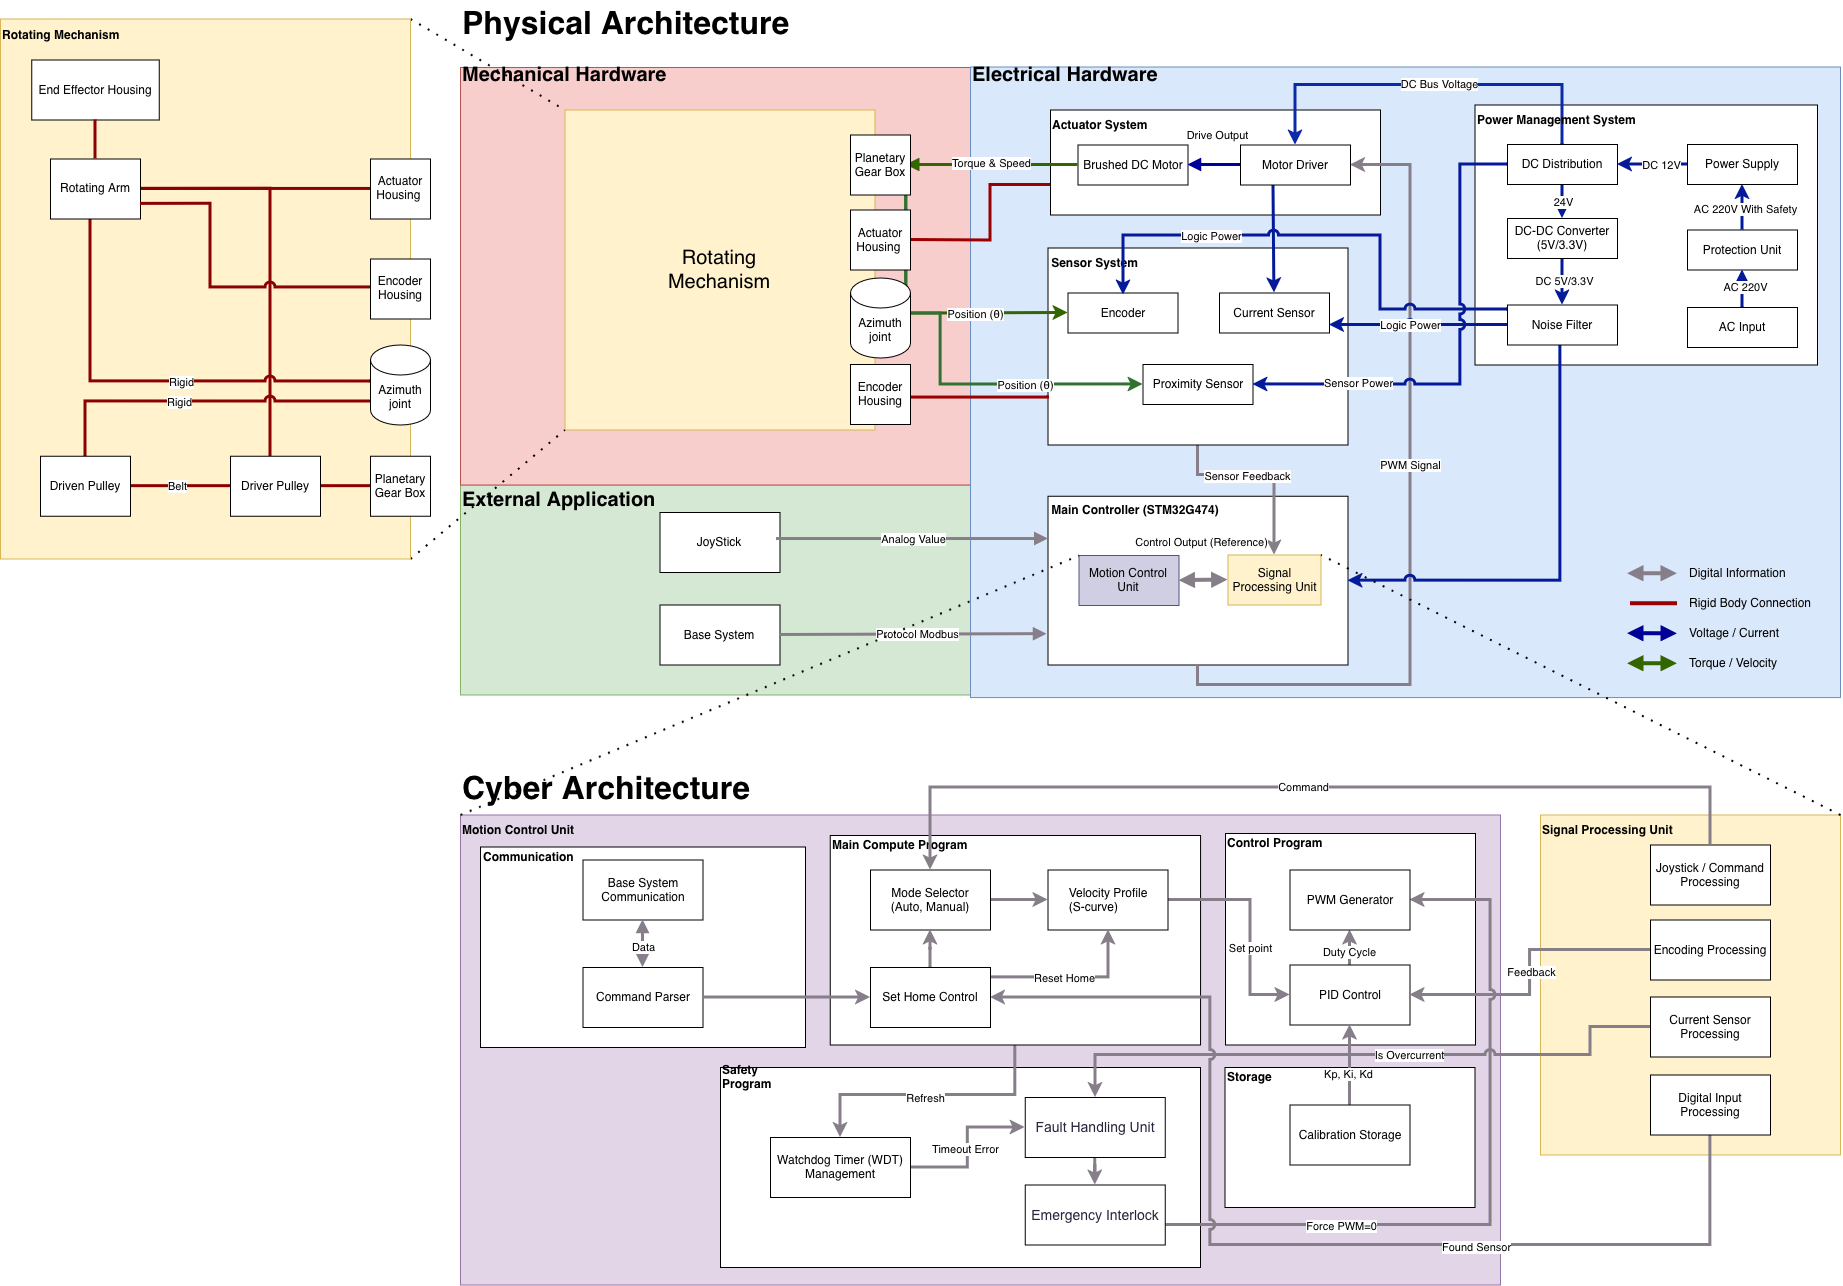
\includegraphics[width=0.95\textwidth]{images/System_Architecture.png}
  \caption{System Architecture ของระบบ Circular Pick and Place Robot
           แสดง Physical Architecture และ Cyber Architecture}
  \label{fig:system_overview}
\end{figure}

% --- Physical Architecture ---
\subsubsection*{Physical Architecture}

Physical Architecture อธิบายถึงฮาร์ดแวร์จริงของระบบและความสัมพันธ์ระหว่างชิ้นส่วนต่าง ๆ
โดยแบ่งออกเป็น 4 ส่วนหลัก ดังนี้

\paragraph{Rotating Mechanism (กลไกหมุน)}
คือส่วนที่แปลงพลังงานไฟฟ้าจากมอเตอร์ให้กลายเป็นการเคลื่อนที่เชิงมุมของแขนกล
โดยมีลำดับการส่งกำลังดังนี้

\begin{itemize}
  \item \textbf{มอเตอร์ต้นกำลัง:}
        ใช้ ZGX60RMM DC Brushed Motor ขนาด 24V 250 RPM
        ซึ่งเป็นชุด Gearmotor ที่มี Planetary Gearbox ในตัว
        เมื่อจ่ายไฟ 24V มอเตอร์จะหมุนและส่งแรงบิดออกมาที่เพลา Output

  \item \textbf{ระบบสายพาน HTD5M:}
        แรงบิดจากเพลา Output ของ Gearmotor ถูกส่งต่อผ่านสายพาน HTD5M (Timing Belt)
        ซึ่งมีการกำหนดอัตราทดเพิ่มเติมอีก 3:1 โดยใช้ Driver Pulley 24 ฟัน
        ขับ Driven Pulley 70 ฟัน สายพานชนิดนี้มีฟันที่ขบกับพูลเลย์โดยตรง
        จึงไม่เกิดการ Slip ไม่ว่าจะรับโหลดเท่าใด
        และมี Idler Pulley ด้านข้าง Slack Side เพื่อรักษาแรงดึงสายพานให้คงที่ตลอดการทำงาน

  \item \textbf{Azimuth Joint และแขนกล:}
        กำลังจากสายพานถูกส่งเข้าสู่ Azimuth Joint ซึ่งเป็นแกนหมุนหลักของระบบ
        ติดตั้ง Taper Bearing และ Single Row Deep Groove Bearing
        เพื่อรับทั้ง Radial Load จากน้ำหนักแขนกล และ Axial Load จากการหมุน
        แขนกลที่ยื่นออกจาก Azimuth Joint ทำจาก Galvanized Steel Square Tube
        ขนาด $25 \times 25$ mm ยาว 500 mm เชื่อมต่อกับ End Effector Housing
        ที่ปลาย ซึ่งรองรับ Gripper ของลูกค้า

  \item \textbf{Encoder ที่ปลายเพลา:}
        ที่ปลายเพลาหลักด้านบนมีการติดตั้ง Encoder Housing
        ไว้รองรับ Incremental Encoder (AMT-103)
        ซึ่งวัดตำแหน่งเชิงมุมโดยตรงที่แกนหมุนหลัก ทำให้ไม่มี Backlash Error
        สะสมจากระบบส่งกำลัง
\end{itemize}

\paragraph{Power Management System (PMS)}
ทำหน้าที่รับไฟฟ้ากระแสสลับจากระบบ และแปลงแจกจ่ายเป็นแรงดันกระแสตรง
ที่เหมาะสมสำหรับแต่ละส่วนของระบบ โดยแบ่งออกเป็น 2 วงจรที่แยกจากกันอย่างชัดเจน

\begin{itemize}
  \item \textbf{วงจรป้องกัน AC Input:}
        ไฟ AC 220V เข้ามาผ่านขั้วต่อ IEC 60320-C14
        จากนั้นผ่านฟิวส์และ Circuit Breaker ก่อนถึง Magnetic Contactor
        ซึ่งเป็นหัวใจของระบบ E-Stop ทางฮาร์ดแวร์
        เมื่อกด E-Stop Contactor จะ De-energize
        และตัดไฟ AC ที่จะไปยัง PSU 24V ทันที ทำให้มอเตอร์หยุดทำงานสมบูรณ์

  \item \textbf{วงจร 24V Power Bus สำหรับมอเตอร์:}
        PSU 24V/10A แปลงไฟ AC เป็น DC 24V
        จ่ายตรงไปยัง Motor Driver (Cytron MD10C)
        ซึ่งจะส่งกำลังต่อไปยังมอเตอร์
        วงจรนี้อยู่หลัง Contactor ดังนั้นเมื่อ E-Stop ถูกกด วงจรนี้จะถูกตัดทันที

  \item \textbf{วงจร 5V Logic Power สำหรับ Controller และ Sensor:}
        PSU 5V/5A แปลงไฟ AC เป็น DC 5V
        จ่ายให้ STM32 Nucleo Board, ESP32, Encoder, Proximity Sensor
        และ Relay Module วงจรนี้ต่อตรงจาก AC Input ก่อน Contactor
        ทำให้เมื่อกด E-Stop ตัว Controller ยังคงมีไฟเลี้ยงอยู่ตามข้อกำหนด E6
        และสามารถรับคำสั่ง Reset ได้

  \item \textbf{DC-DC Step-down Converter:}
        แปลงแรงดันลงมาสำหรับอุปกรณ์ที่ต้องการแรงดันพิเศษ
        เช่น 3.3V สำหรับ Logic Level บางส่วน หรือ 12V สำหรับอุปกรณ์เสริม
        ผ่าน Noise Filter ก่อนเข้า Controller
        เพื่อให้แรงดันสะอาดไม่มีสัญญาณรบกวนจากมอเตอร์
\end{itemize}

\paragraph{Main Controller (STM32G474RE)}
บน Nucleo Board ทำหน้าที่เป็นศูนย์กลางในการประมวลผลทั้งหมด
โดยเชื่อมต่อกับอุปกรณ์รอบข้างผ่าน Peripheral ต่าง ๆ ดังนี้

\begin{itemize}
  \item \textbf{Timer (Quadrature Mode):}
        รับสัญญาณ A, B จาก Encoder นับ Pulse
        เพื่อคำนวณตำแหน่งเชิงมุมและความเร็ว

  \item \textbf{Timer (PWM Mode):}
        สร้างสัญญาณ PWM ส่งไปยัง Motor Driver
        เพื่อควบคุมความเร็วและทิศทางของมอเตอร์

  \item \textbf{ADC:}
        อ่านค่าแรงดันจาก Current Sensor
        เพื่อตรวจสอบกระแสมอเตอร์แบบ Real-time

  \item \textbf{EXTI (External Interrupt):}
        รับสัญญาณจาก Proximity Sensor
        เมื่อแขนกลผ่านตำแหน่ง Home Reference

  \item \textbf{UART:}
        รับ Data Packet จาก ESP32
        ที่ถอดรหัสคำสั่งจาก Joystick มาแล้ว

  \item \textbf{GPIO:}
        ควบคุม Relay Module สำหรับ Solenoid Valve ของ Gripper
        และอ่านสถานะ Mode Selector Switch
\end{itemize}

\paragraph{Sensor System}
ทำหน้าที่เป็นตา-หูของระบบควบคุม ให้ข้อมูล Feedback
ที่จำเป็นสำหรับการทำงานแบบ Closed-Loop

\begin{itemize}
  \item \textbf{AMT-103 Incremental Encoder:}
        ติดตั้งโดยตรงที่เพลาหลักของ Azimuth Joint
        ให้ค่า Resolution สูง ใช้สำหรับ Position Feedback
        และ Velocity Estimation ใน Control Loop

  \item \textbf{Proximity Sensor (Inductive Type):}
        ติดตั้งที่ฐานของ Rotating Mechanism
        ตรวจจับ Metal Flag บนแขนกลเมื่อผ่านตำแหน่ง Home Reference
        ใช้สำหรับการ Homing ครั้งแรกและการ Reset ตำแหน่งอ้างอิง

  \item \textbf{Current Sensor:}
        ต่ออยู่ในวงจร 24V ของมอเตอร์
        อ่านค่ากระแสแบบ Real-time ส่งให้ Fault Handling Unit
        ตรวจสอบว่ากระแสเกินพิกัดหรือไม่
        ซึ่งอาจเป็นสัญญาณของการชนหรือ Mechanical Jam
\end{itemize}

% --- Cyber Architecture ---
\subsubsection*{Cyber Architecture}

Cyber Architecture อธิบายโครงสร้างซอฟต์แวร์ภายใน STM32G474RE
ซึ่งทำงานแบบ Real-time Closed-Loop แบ่งออกเป็น 4 โมดูลที่ทำงานสัมพันธ์กัน

\paragraph{Signal Processing Unit}
คือชั้นแรกที่รับข้อมูลดิบจากฮาร์ดแวร์และแปลงให้อยู่ในรูปแบบที่โมดูลอื่นนำไปใช้ได้ทันที
ประกอบด้วย 4 ส่วนย่อย

\begin{itemize}
  \item \textbf{Encoding Processing:}
        รับสัญญาณ Quadrature A และ B จาก Encoder ผ่าน Timer ของ STM32
        นับ Pulse และแปลงเป็นค่ามุม $\theta$ (องศาหรือ Radian)
        และความเร็วเชิงมุม $\omega$ โดยใช้การคำนวณ Differentiation
        ของตำแหน่ง ค่า $\theta_{\text{actual}}$ ที่ได้นี้จะถูกส่งไปยัง
        Summing Junction ของ Control Program เพื่อใช้เป็น Position Feedback

  \item \textbf{Current Sensor Processing:}
        อ่านค่า ADC จาก Current Sensor แปลงเป็นค่ากระแส (Ampere)
        และกรองสัญญาณรบกวนด้วย Moving Average Filter
        ก่อนส่งต่อไปยัง Fault Handling Unit ใน Safety Program

  \item \textbf{Joystick / Command Processing:}
        รับ Data Packet จาก ESP32 ผ่าน UART ตรวจสอบ Checksum ของ Packet
        ถอดรหัสออกเป็นคำสั่งแต่ละประเภท เช่น หมุนซ้าย หมุนขวา Pick Place Home Emergency
        แล้วส่งต่อไปยัง Command Parser ใน Main Compute Program

  \item \textbf{Digital Input Processing:}
        อ่านและ Debounce สัญญาณดิจิทัลทั้งหมด ได้แก่ Proximity Sensor (EXTI Interrupt),
        Mode Selector Switch และ Encoder Index Pulse
        เพื่อป้องกัน False Trigger จาก Contact Bounce
\end{itemize}

\paragraph{Main Compute Program}
คือ Logic หลักของระบบ ทำหน้าที่ตัดสินใจว่าระบบจะทำอะไรในแต่ละขณะ

\begin{itemize}
  \item \textbf{Mode Selector:}
        อ่านสถานะจาก Mode Selector Switch และคำสั่งจาก Joystick หรือ Modbus
        เพื่อตัดสินใจว่าระบบอยู่ในโหมด Manual หรือ Auto
        ในโหมด Manual คำสั่งจะมาจาก Joystick โดยตรง
        ในโหมด Auto คำสั่งจะมาจาก Base System ผ่าน Modbus

  \item \textbf{Velocity Profile (S-Curve):}
        เมื่อได้รับคำสั่งให้เคลื่อนที่ไปยังตำแหน่งเป้าหมาย
        โมดูลนี้จะสร้าง Trajectory ที่กำหนดว่าแต่ละช่วงเวลา
        ควรอยู่ที่ตำแหน่งใด โดยใช้ S-Curve Profile ที่จำกัด Jerk
        ทำให้ความเร็วเพิ่มและลดแบบค่อยเป็นค่อยไป
        ลด Mechanical Shock และควบคุม Overshoot
        ค่าที่ Output ออกมาจาก Velocity Profile คือ $\theta_{\text{reference}}$
        ณ แต่ละ Timestep ซึ่งถูกส่งไปยัง Summing Junction เป็น Set Point

  \item \textbf{Set Home Control:}
        เมื่อได้รับคำสั่ง Set Home ระบบจะบันทึกค่า Encoder Count ปัจจุบันลงใน
        Calibration Storage และกำหนดให้ตำแหน่งนั้นเป็นจุดอ้างอิง (Zero Point)
        สำหรับการคำนวณตำแหน่งทั้งหมดต่อจากนั้น
        เมื่อได้รับคำสั่ง Reset Home ระบบจะหมุนแขนกลจนกว่า Proximity Sensor
        จะตรวจจับ Metal Flag แล้วกำหนดตำแหน่งนั้นเป็น Home

  \item \textbf{Command Parser และ Auto Sequence:}
        ในโหมด Auto รับคำสั่งจาก Base System ผ่าน Modbus
        แล้วแปลงเป็น Task ลำดับการทำงาน คือ
        ตรวจสอบ Home $\rightarrow$ เคลื่อนที่ไปจุดหยิบ $\rightarrow$ Pick
        $\rightarrow$ เคลื่อนที่ไปจุดวาง $\rightarrow$ Place $\rightarrow$ ทำซ้ำ
        จนครบ 5 รอบ $\rightarrow$ กลับ Home $\rightarrow$ ส่งสถานะ Complete
        ไปยัง Base System
\end{itemize}

\paragraph{Control Program}
รับ Set Point จาก Main Compute Program และ Feedback จาก Signal Processing Unit
เพื่อคำนวณ Output ที่จะส่งไปควบคุมมอเตอร์

\begin{itemize}
  \item \textbf{PID Control:}
        คำนวณ Error ระหว่าง $\theta_{\text{reference}}$ และ $\theta_{\text{actual}}$
        แล้วคำนวณ Control Output ด้วยอัลกอริทึม PID
        ที่ออกแบบให้ได้ Settling Time $\leq 0.5$ s และ Overshoot $\leq 1\%$
        ตามข้อกำหนด P5 และ P6

  \item \textbf{PWM Generator:}
        แปลงค่า Control Output จาก PID เป็น Duty Cycle
        ของสัญญาณ PWM ที่ส่งไปยัง Motor Driver
        เพื่อควบคุมความเร็วและทิศทางการหมุนของมอเตอร์
\end{itemize}

\paragraph{Safety Program}
ทำงานอยู่เบื้องหลังตลอดเวลา มีสิทธิ์ Override คำสั่งจากทุกโมดูล
เพื่อปกป้องทั้งตัวเครื่องและผู้ปฏิบัติงาน

\begin{itemize}
  \item \textbf{Watchdog Timer (WDT):}
        WDT เป็น Timer ฮาร์ดแวร์ภายใน STM32 ที่ต้องได้รับการ Reset (Kick)
        ภายในระยะเวลาที่กำหนดทุก ๆ Cycle ของโปรแกรม
        หากโปรแกรมหยุดทำงาน ค้าง หรือเข้าสู่ Infinite Loop ด้วยเหตุใดก็ตาม
        WDT จะหมดเวลาและทำการ Reset STM32 ทั้งระบบโดยอัตโนมัติ
        ทำให้ระบบกลับสู่สถานะเริ่มต้นที่ปลอดภัย

  \item \textbf{Fault Handling Unit:}
        ตรวจสอบค่ากระแสจาก Current Sensor Processing ทุก Cycle
        หากกระแสเกิน Threshold ที่กำหนดไว้ เช่น เกิดการชนหรือ Mechanical Jam
        จะส่งสัญญาณ Fault ไปยัง Emergency Interlock ทันที
        พร้อมบันทึกรหัส Error ลงใน Storage เพื่อให้ผู้ปฏิบัติงานสามารถตรวจสอบสาเหตุ
        ในภายหลัง

  \item \textbf{Emergency Interlock:}
        เป็นจุดรวมของสัญญาณ Fault ทุกประเภท ไม่ว่าจะมาจาก Fault Handling Unit
        (Overcurrent), WDT Timeout หรือคำสั่ง E-Stop จาก Joystick หรือปุ่มบนตู้ไฟ
        เมื่อได้รับสัญญาณจากแหล่งใดก็ตาม Emergency Interlock จะบังคับให้
        PWM Generator ส่งสัญญาณ Force PWM = 0 ทันที
        ทำให้มอเตอร์หยุดทำงานโดยไม่รับคำสั่งอื่นใดอีก
        จนกว่าจะได้รับการ Reset อย่างถูกต้อง
\end{itemize}

% ---------------------------------------------------------------------------
\subsection{สรุป System Requirements}

เพื่อให้สอดคล้องกับขอบเขตโครงการในหัวข้อ 2.2 คณะผู้จัดทำได้กำหนดข้อกำหนดความต้องการ
ทางเทคนิคสำหรับใช้อ้างอิงในการออกแบบและทดสอบระบบ ดังตารางต่อไปนี้
โดยแบ่งออกเป็น 5 หมวดหมู่ ได้แก่
M (Mechanical) = โครงสร้างและกลไก,
P (Performance) = สมรรถนะการทำงาน,
A (Accuracy \& Control) = ความแม่นยำและการควบคุม,
E (Electrical \& Interface) = ระบบไฟฟ้าและการเชื่อมต่อ, และ
J (Joystick) = การควบคุมผ่านจอยสติ๊ก

\begin{table}[H]
  \centering
  \caption{สรุป System Requirements ทั้ง 32 ข้อ}
  \label{tab:req_summary}
  \small
  \begin{tabular}{|c|c|p{10cm}|}
    \hline
    \textbf{Req ID} & \textbf{หมวด} & \textbf{คำอธิบาย} \\
    \hline
    M1  & Mechanical & ขนาดฐานไม่เกิน $200 \times 200$ mm \\
    \hline
    M2  & Mechanical & Actuator และ Sensor สามารถยื่นออกนอกขนาดฐานได้ \\
    \hline
    M3  & Mechanical & End Effector รวมชิ้นงาน รับน้ำหนักได้สูงสุด 2 kg \\
    \hline
    M4  & Mechanical & ใช้ Brushed DC Motor พร้อม Incremental Encoder \\
    \hline
    M5  & Mechanical & อายุใช้งานทนทาน $\geq 3$ รอบการทดสอบ (รอบละ 1 ชม.) \\
    \hline
    M6  & Mechanical & ชิ้นส่วนรับแรงห้ามใช้ 3D Print เด็ดขาด \\
    \hline
    M7  & Mechanical & ยึดฐานสแตนเลส AISI304 ลูกค้าด้วยสกรู M8 เหล็กกรมดำ \\
    \hline
    M8  & Mechanical & เพลาต่อ Encoder ลูกค้า $\varnothing$ 8 mm (สูง 400 mm, ยื่นจากตัวเครื่อง $\geq$ 20 mm) \\
    \hline
    M9  & Mechanical & หมุนต่อเนื่องได้ $\geq 540^{\circ}$ โดยสายไฟไม่พันหรือพันกัน \\
    \hline
    M10 & Mechanical & จุดต่ำสุดของกริปเปอร์ต้องไม่ชนกับ Connection Rod \\
    \hline
    P1  & Performance & ทำงานครบ 1 รอบ (หยิบวาง 5 ชิ้น + กลับ Homing) ใน $\leq$ 35 วินาที \\
    \hline
    P2  & Performance & Gripper ใช้เวลาหยิบ $\sim$2 วินาที และวาง $\sim$2 วินาที \\
    \hline
    P3  & Performance & ความเร็วเชิงมุม (Velocity) $\geq 2.9$ rad/s และ $\leq 5.76$ rad/s \\
    \hline
    P4  & Performance & ความเร่งเชิงมุม (Acceleration) $\geq 2.0$ rad/s$^2$ และ $\leq 5$ rad/s$^2$ \\
    \hline
    P5  & Performance & ระยะเวลาเข้าสู่สภาวะคงตัว (Settling Time) $\leq 0.5$ วินาที \\
    \hline
    P6  & Performance & การเคลื่อนที่ที่พุ่งเกินเป้าหมาย (Overshoot) $\leq 1\%$ \\
    \hline
    P7  & Performance & รองรับการทดสอบทั้งแบบมีโหลด (2 kg) และไม่มีโหลด \\
    \hline
    A1  & Accuracy \& Control & ต้องสวมเพลาขนาด 12 mm ลงในรู 14 mm ได้ถูกต้อง \\
    \hline
    A2  & Accuracy \& Control & ความแม่นยำซ้ำ 100 รอบ (Precision) คลาดเคลื่อน $\leq \pm 0.1^{\circ}$ \\
    \hline
    A3  & Accuracy \& Control & ผู้ใช้สามารถ Set จุด Homing เองได้ หลังตั้งค่าตั้งกับฐาน \\
    \hline
    A4  & Accuracy \& Control & สั่งงานได้ 2 แบบ: (1) ระบุองศา (2) ระบุลำดับตำแหน่งจาก Homing \\
    \hline
    A5  & Accuracy \& Control & หากสั่งงานนอกระยะ (Out-of-Workspace) ระบบต้องแจ้ง Error หรือป้องกันไว้ \\
    \hline
    E1  & Electrical \& Interface & สื่อสารผ่าน Modbus \\
    \hline
    E2  & Electrical \& Interface & ใช้ STM32 เป็น Controller หลัก (มีตัวรองได้) \\
    \hline
    E3  & Electrical \& Interface & สายต่อตู้ไฟ: ท่อลม $\varnothing$ 4 mm (4 เส้น), สาย GX (1 เส้น), สาย Motor (1 เส้น) \\
    \hline
    E4  & Electrical \& Interface & ตู้ไฟมาตรฐานอุตสาหกรรม: จัดสายสวยงาม, ติด Label, มี Schematic \\
    \hline
    E5  & Electrical \& Interface & หน้าตู้ไฟมีไฟแสดงสถานะ: Power On/Off และ Emergency \\
    \hline
    E6  & Electrical \& Interface & E-Stop: ตัดการเคลื่อนที่แต่ Controller หลักยังมีไฟเลี้ยง (Reset ได้) \\
    \hline
    E7  & Electrical \& Interface & มีวงจรป้องกัน: ไฟกระชาก, กระแสเกิน, แรงดันตก \\
    \hline
    E8  & Electrical \& Interface & สลับโหมดการทำงาน Manual / Auto ได้ \\
    \hline
    E9  & Electrical \& Interface & สัญญาณ Feedback กริปเปอร์: ขึ้นสุด, ลงสุด, หนีบสำเร็จ, ปล่อยสำเร็จ \\
    \hline
    J1  & Joystick & จอยสติ๊กมีปุ่ม: กลับ Homing, Start, E-Stop \\
    \hline
  \end{tabular}
\end{table}
% ============================================================================
% FILE: sections/02_design.tex
% PURPOSE: การออกแบบทั้ง 3 ด้าน Mechanical / Electronics / Control
% ============================================================================

\section{การออกแบบระบบ (System Design)}

% ============================================================
\subsection{การออกแบบเชิงกล (Mechanical Design)}
% ============================================================

\subsubsection{สถาปัตยกรรมเชิงกลโดยรวม}
% อธิบาย Layout ของ Arm, Base, Shaft, Pulley, Belt

\begin{figure}[H]
  \centering
%   \includegraphics[width=0.75\textwidth]{images/mech_cad_overview.png}
  % [ใส่ภาพ CAD Assembly ด้านข้าง/ด้านบน แสดง Layout ทั้งหมด]
  \caption{CAD Assembly ของระบบเชิงกล}
  \label{fig:mech_cad}
\end{figure}

\subsubsection{การคำนวณเพลา (Shaft Calculation)}
% สรุปสมการและผลการคำนวณเพลา
% แรงที่กระทำ, สมการ Bending, Factor of Safety
% ค่าที่ได้: [ใส่ค่าจริง]

\begin{table}[H]
  \centering
  \caption{สรุปผลการคำนวณเพลา}
  \label{tab:shaft_calc}
  % [ตาราง: พารามิเตอร์ | สัญลักษณ์ | ค่าที่คำนวณ | หน่วย]
\end{table}

\subsubsection{การคำนวณสายพาน (Belt Calculation)}
% แรงดึงสายพาน, Tension Ratio, Belt Life
% ค่าที่ได้: [ใส่ค่าจริง]

\begin{table}[H]
  \centering
  \caption{สรุปผลการคำนวณสายพาน}
  \label{tab:belt_calc}
  % [ตาราง: พารามิเตอร์ | สัญลักษณ์ | ค่าที่คำนวณ | หน่วย]
\end{table}

\subsubsection{การเลือก Bearing}
% ประเภท Bearing ที่ใช้, Load Rating, Life Calculation (L10)
% ค่าที่ได้: [ใส่ค่าจริง]

\subsubsection{การวิเคราะห์การโก่งตัว (Deflection Analysis)}
% ผลการคำนวณ Deflection ทางทฤษฎีและ FEA
% FEA ได้ $\delta_{\text{total}} = 0.237$ mm (ผ่านเกณฑ์ $< 1$ mm ตาม M3)

\begin{figure}[H]
  \centering
%   \includegraphics[width=0.80\textwidth]{images/fea_result.png}
  % [ใส่ภาพ FEA จาก SolidWorks แสดง Displacement Contour]
  \caption{ผล FEA การโก่งตัวของ Arm ที่โหลด 2 kg}
  \label{fig:fea_deflection}
\end{figure}

\begin{table}[H]
  \centering
  \caption{เปรียบเทียบผลการโก่งตัวจากทฤษฎีและ FEA}
  \label{tab:deflection_compare}
  % [ตาราง: วิธี | ค่า delta (mm) | เกณฑ์ | ผลการตรวจสอบ]
\end{table}

\subsubsection{Motion Profile การเคลื่อนที่ (S-Curve)}
% การคำนวณ Motion Profile แบบ S-Curve
% เวลารวม: 34.39 s (ทฤษฎี <= 35 s ตาม P1)

\begin{figure}[H]
  \centering
%   \includegraphics[width=0.85\textwidth]{images/motion_profile_scurve.png}
  % [ใส่ภาพกราฟ S-Curve: Position, Velocity, Acceleration vs Time]
  \caption{S-Curve Motion Profile ของการเคลื่อนที่ในหนึ่งรอบ}
  \label{fig:motion_profile}
\end{figure}

\begin{table}[H]
  \centering
  \caption{สรุปพารามิเตอร์ Motion Profile}
  \label{tab:motion_profile_params}
  % [ตาราง: พารามิเตอร์ | ค่าทฤษฎี | ค่าจริง | หน่วย]
\end{table}

% ============================================================
\subsection{การออกแบบระบบไฟฟ้าและอิเล็กทรอนิกส์ (Electronics Design)}
% ============================================================

\subsubsection{สถาปัตยกรรมไฟฟ้าโดยรวม}

ระบบไฟฟ้าแบ่งออกเป็น 2 วงจรหลักที่แยกจากกันอย่างชัดเจน
เพื่อให้ระบบ E-Stop ตัดเฉพาะกำลังไฟของมอเตอร์
โดยที่ Controller ยังคงมีไฟเลี้ยงอยู่ตามข้อกำหนด E6

\textbf{วงจร High Power (24\,V Motor Bus):}
ไฟ AC 220\,V เข้ามาผ่าน Circuit Breaker CB1 แล้วจ่ายให้ PSU 24\,V/10\,A
Output ของ PSU ผ่าน NC Contact ของปุ่ม Emergency Stop
แล้วต่อเข้า Coil ของ Magnetic Contactor
เมื่อ Contactor ดึง หน้าสัมผัสหลักจะปิดและจ่ายไฟ 24\,V
ไปยัง Motor Driver Cytron MD10C เพื่อขับมอเตอร์
เมื่อกด Emergency Stop NC Contact เปิดออก
Contactor De-energize และตัดไฟมอเตอร์ทันที

\textbf{วงจร Logic Power (5\,V Control Bus):}
PSU 5\,V/5\,A ต่อตรงจาก AC 220\,V ก่อนถึง Emergency Stop
ทำให้ STM32, ESP32, Encoder, Proximity Sensor
และ Relay Module ยังคงมีไฟเลี้ยงอยู่แม้กด Emergency Stop
ระบบจึงสามารถรับคำสั่ง Reset และแสดงสถานะผ่าน Pilot Lamp ได้ตลอดเวลา

สัญญาณดิจิทัลทุกเส้นที่เชื่อมระหว่าง High Voltage Side
และ Logic Side ผ่าน Optocoupler Module 8 ช่อง
เพื่อแยก Ground และป้องกัน Noise จากมอเตอร์
ไม่ให้รบกวนการทำงานของ STM32

\begin{figure}[H]
  \centering
  % [ใส่ภาพ Electrical Block Diagram]
  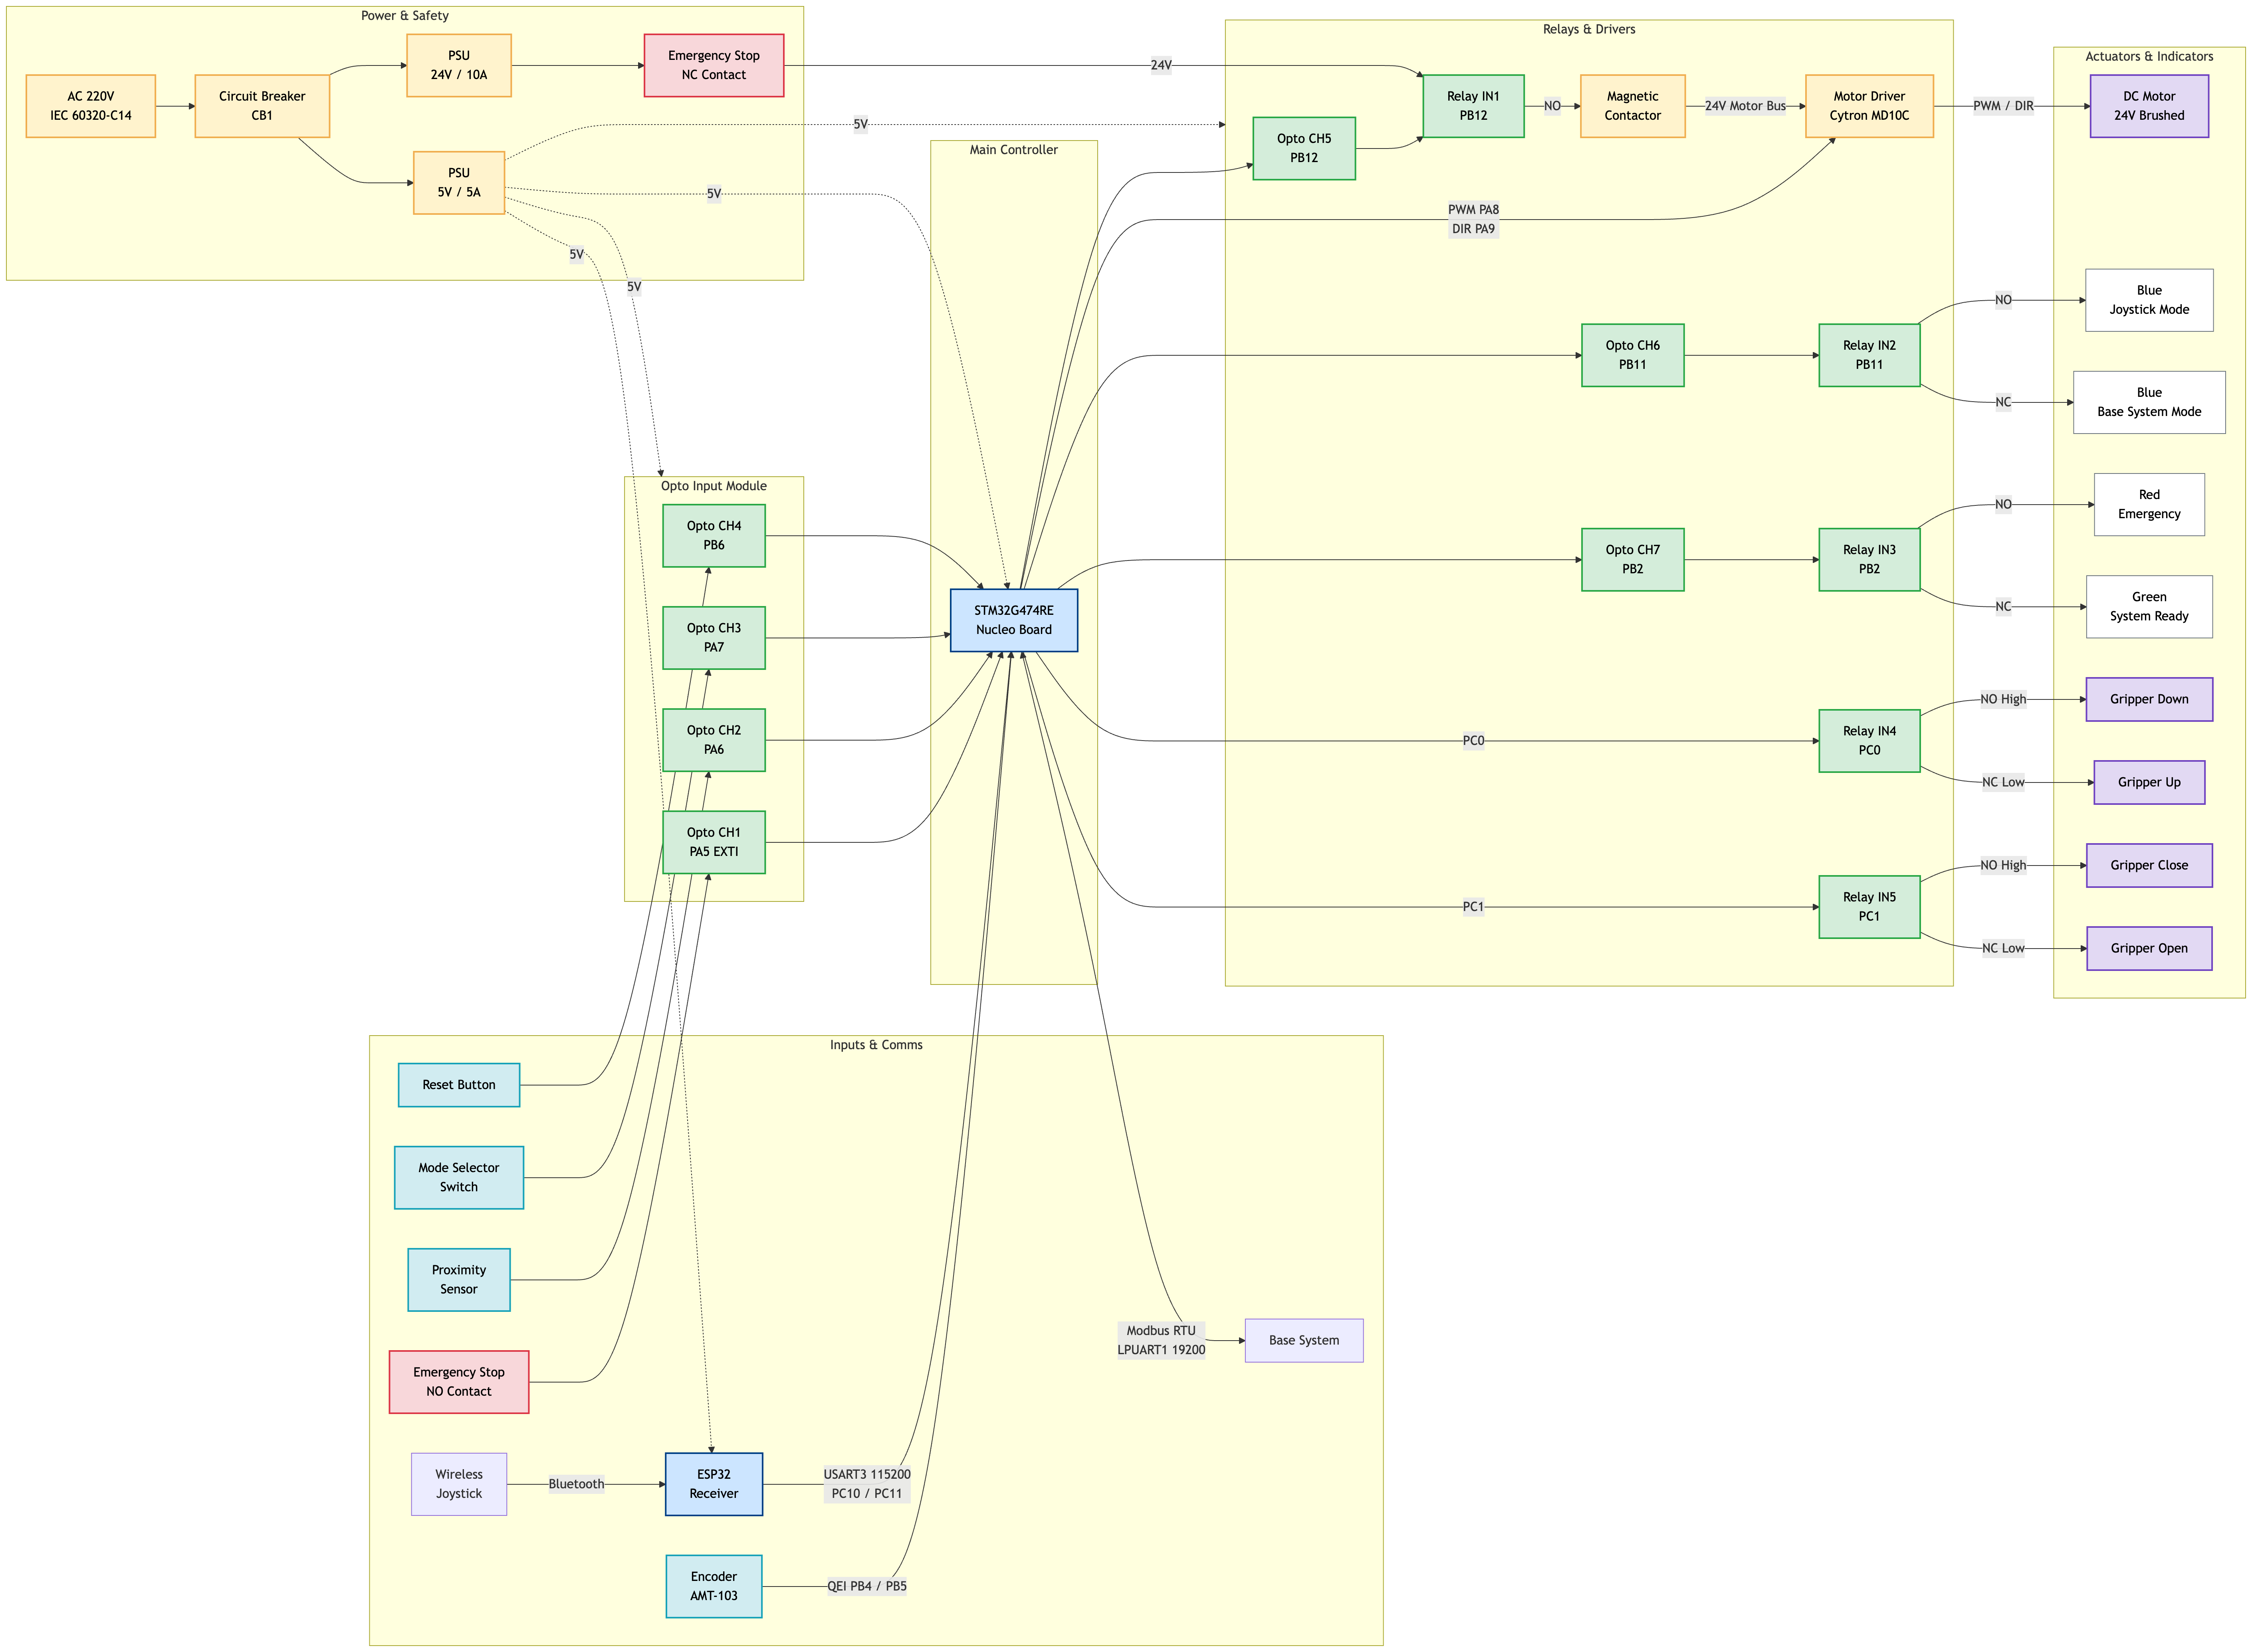
\includegraphics[width=0.95\textwidth]{images/electric_block.png}
  \caption{Electrical Block Diagram แสดงการแจกจ่ายกำลังไฟฟ้า
           และการเชื่อมต่อ Signal ของระบบ}
  \label{fig:elec_block}
\end{figure}

% ============================================================
\subsubsection{Schematic ตู้ควบคุม}
% ============================================================

Schematic ออกแบบด้วย KiCad 9.0.0 ดังแสดงใน\cref{fig:schematic}
ประกอบด้วยส่วนประกอบหลัก ได้แก่
STM32G474RE Nucleo Board เป็น Main Controller,
ESP32-DEVKITC-32UE สำหรับรับสัญญาณ Joystick ผ่าน Bluetooth,
Optocoupler Module 8 ช่อง, Relay Module 8 ช่อง,
Magnetic Contactor, PSU 24\,V/10\,A และ PSU 5\,V/5\,A

\begin{figure}[H]
  \centering
  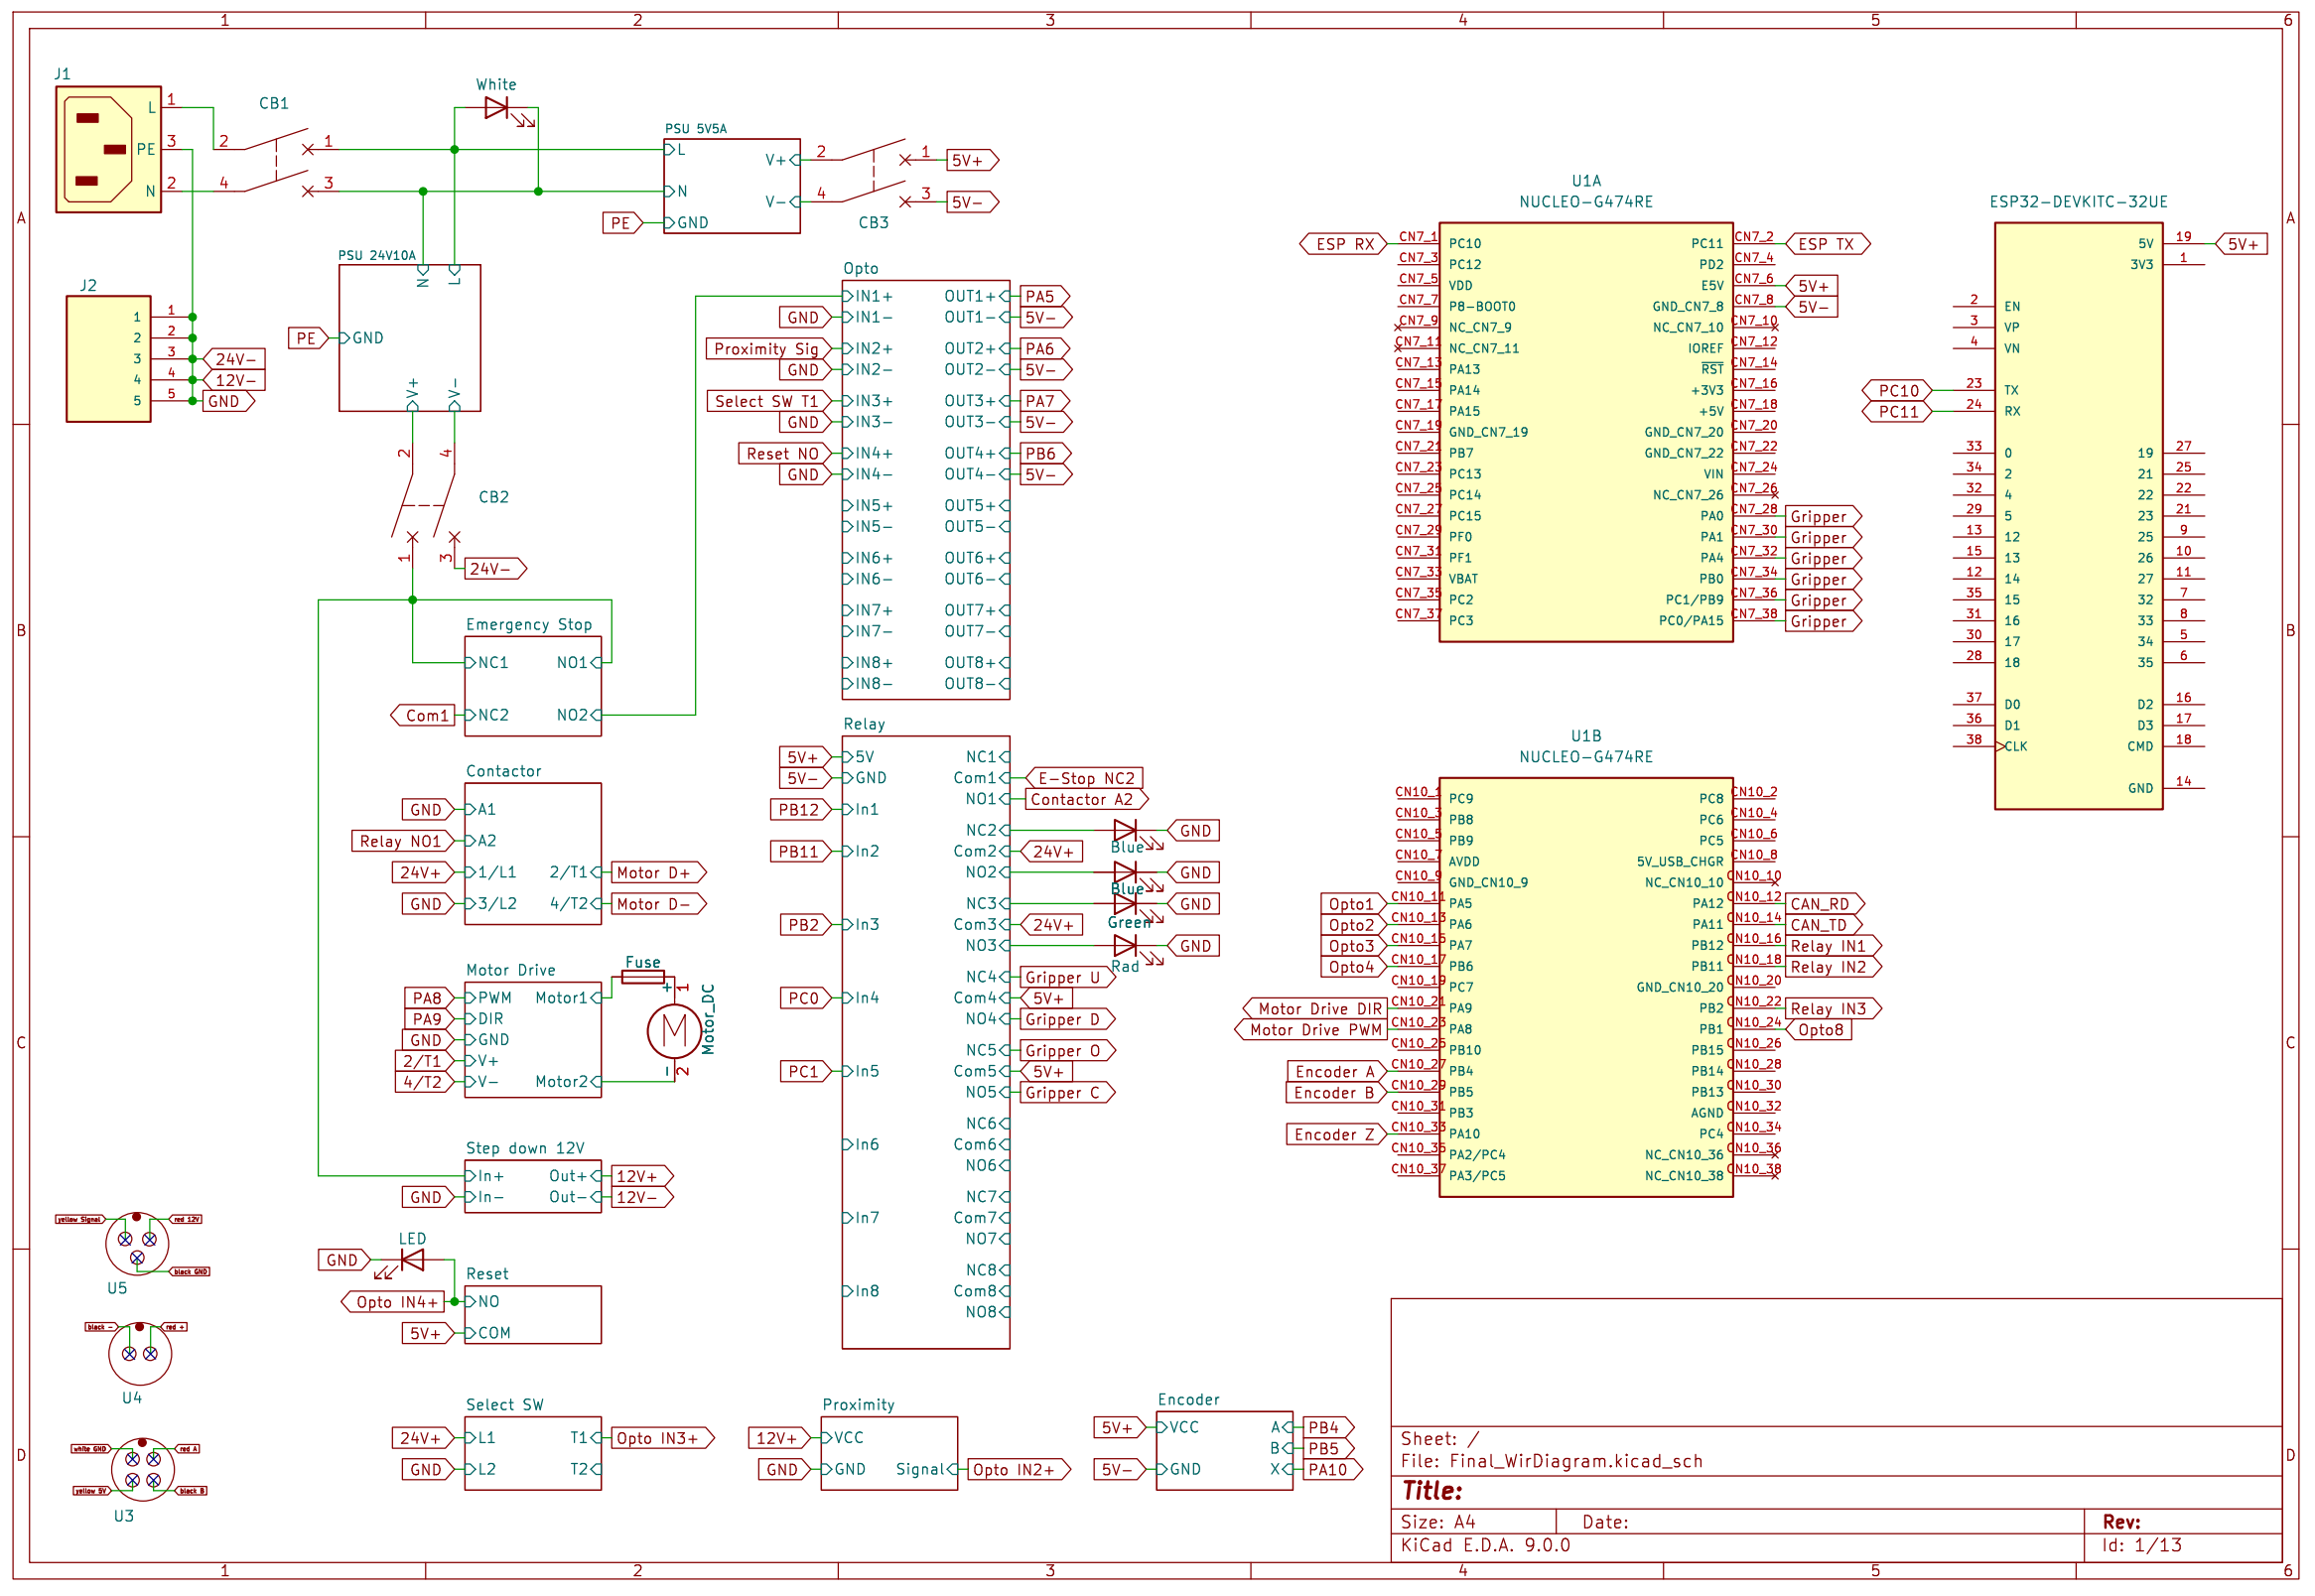
\includegraphics[width=0.95\textwidth]{images/electrical_schematic.png}
  \caption{Electrical Schematic ของตู้ควบคุมทั้งระบบ ออกแบบด้วย KiCad 9.0.0}
  \label{fig:schematic}
\end{figure}

\subsubsection{การออกแบบ PCB (PCB Design)}

PCB ออกแบบด้วย KiCad 9.0.0 เพื่อรวม STM32G474RE Nucleo Board,
ESP32-DEVKITC-32UE, Optocoupler Module, Relay Module,
Encoder Connector และ Motor Driver Connector ไว้บน Board เดียวกัน
เพื่อลดจำนวนสายเชื่อมต่อภายในตู้ควบคุมและเพิ่มความเป็นระเบียบ

\begin{figure}[H]
  \centering
  \begin{subfigure}[b]{0.48\textwidth}
    \centering
    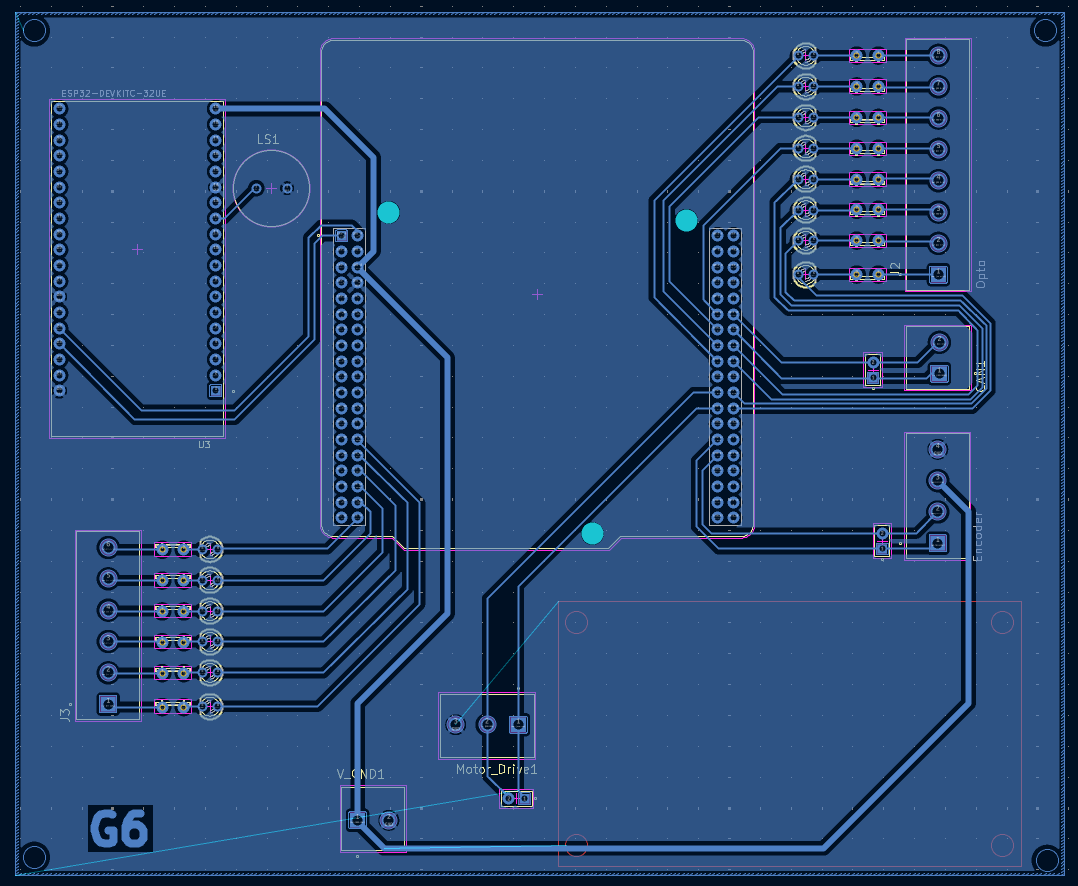
\includegraphics[width=\textwidth]{images/pcb_layout.png}
    \caption{PCB Layout (KiCad PCB Editor)}
    \label{fig:pcb_layout}
  \end{subfigure}
  \hfill
  \begin{subfigure}[b]{0.48\textwidth}
    \centering
    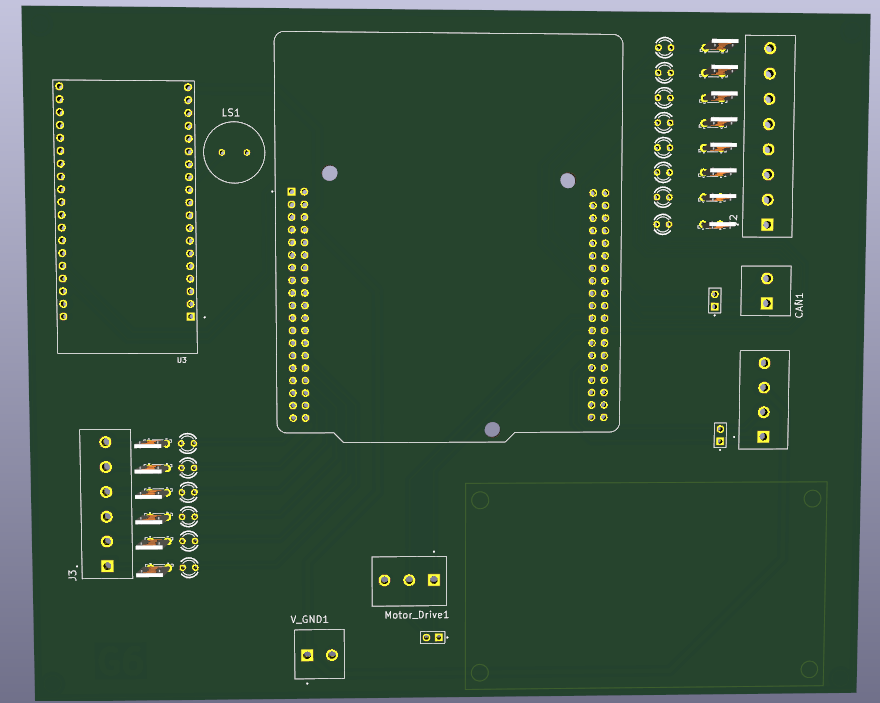
\includegraphics[width=\textwidth]{images/pcb_3d.png}
    \caption{PCB 3D Render}
    \label{fig:pcb_3d}
  \end{subfigure}
  \caption{การออกแบบ PCB สำหรับระบบควบคุม}
  \label{fig:pcb_design}
\end{figure}

% ============================================================
\subsubsection{การออกแบบวงจรป้องกัน (Protection Circuit)}
% ============================================================

ระบบมีวงจรป้องกันหลายชั้นตามข้อกำหนด E7 ดังนี้

\textbf{การป้องกัน Overcurrent:}
Circuit Breaker CB1 ทำหน้าที่ป้องกันกระแสเกินพิกัด
ในวงจร AC Input และ CB2 ป้องกันวงจร 24\,V
นอกจากนี้ Cytron MD10C มีวงจรป้องกัน Overcurrent ในตัว
และ Firmware ของ STM32 ตรวจสอบกระแสจาก Current Sensor
ทุก Control Cycle หากเกิน Threshold จะสั่งตัด PWM ทันที

\textbf{การป้องกัน Surge และ Noise:}
Optocoupler Module แยก Ground ระหว่าง High Power Side
และ Logic Side ป้องกัน Surge จากมอเตอร์ไม่ให้ทำลาย STM32
Fuse ต่ออนุกรมในวงจร Motor Driver
เพื่อป้องกันความเสียหายเมื่อเกิด Short Circuit

\textbf{Emergency Stop Hardware Interlock:}
E-Stop ทำงานในระดับ Hardware โดยตรง
ไม่ผ่าน Firmware ทำให้ไม่สามารถ Override ได้แม้ Software ค้าง
NC Contact ของปุ่ม E-Stop ต่ออยู่ใน Series กับ Coil ของ Contactor
เมื่อกด E-Stop หรือสายหลุด Contactor จะ De-energize ทันที
(Fail-Safe Design)

% ============================================================
\subsubsection{การออกแบบวงจร Optocoupler และ Relay}
% ============================================================

Optocoupler Module ทำหน้าที่แปลงสัญญาณระหว่าง
High Voltage Side (24\,V) และ Logic Side (3.3\,V/5\,V ของ STM32)
ใน 2 ทิศทาง ดังแสดงในตารางที่~\ref{tab:opto_mapping}

\begin{table}[H]
  \centering
  \caption{Optocoupler Module Channel Mapping}
  \label{tab:opto_mapping}
  \begin{tabular}{cclll}
    \toprule
    Channel & ทิศทาง & สัญญาณ & STM32 Pin & Mode \\
    \midrule
    CH1 & Input  & Emergency Stop      & PA5  & EXTI Interrupt \\
    CH2 & Input  & Proximity Sensor    & PA6  & GPIO Input \\
    CH3 & Input  & Mode Selector SW    & PA7  & GPIO Input \\
    CH4 & Input  & Reset Button        & PB6  & GPIO Input \\
    CH5 & Output & Relay IN1 (Motor)   & PB12 & GPIO Output \\
    CH6 & Output & Relay IN2 (Mode Lamp) & PB11 & GPIO Output \\
    CH7 & Output & Relay IN3 (Status Lamp) & PB2 & GPIO Output \\
    CH8 & Output & ยังไม่กำหนด        & PB1  & GPIO Output \\
    \bottomrule
  \end{tabular}
\end{table}

Relay Module รับคำสั่งจาก STM32 ผ่าน Optocoupler
และควบคุมอุปกรณ์กำลังสูงดังแสดงในตารางที่~\ref{tab:relay_mapping}

\begin{table}[H]
  \centering
  \caption{Relay Module Channel Mapping}
  \label{tab:relay_mapping}
  \begin{tabular}{cclll}
    \toprule
    Relay & STM32 Pin & COM & NO & NC \\
    \midrule
    IN1 & PB12 & 24\,V (E-Stop NC2) & Contactor A1       & --                  \\
    IN2 & PB11 & 24\,V PSU          & Pilot Blue Joystick & Pilot Blue Base     \\
    IN3 & PB2  & 24\,V PSU          & Pilot Red Emergency & Pilot Green Ready   \\
    IN4 & PC0  & 5\,V PSU           & Gripper Down (High) & Gripper Up (Low)    \\
    IN5 & PC1  & 5\,V PSU           & Gripper Close (High)& Gripper Open (Low)  \\
    \bottomrule
  \end{tabular}
\end{table}

% ============================================================
\subsubsection{STM32 Pin Assignment}
% ============================================================

ตารางที่~\ref{tab:pin_assignment} สรุป Pin Assignment ทั้งหมด
ของ STM32G474RE แบ่งตาม Subsystem

\begin{table}[H]
  \centering
  \caption{STM32G474RE Pin Assignment ของระบบ}
  \label{tab:pin_assignment}
  \begin{tabular}{lllll}
    \toprule
    Pin & Function & Mode & เชื่อมต่อกับ \\
    \midrule
    \multicolumn{4}{l}{\textit{Motor Control}} \\
    PA8 & PWM Output & TIM1 CH1         & Motor Driver PWM \\
    PA9 & DIR Output & GPIO Push-Pull    & Motor Driver DIR \\
    \midrule
    \multicolumn{4}{l}{\textit{Encoder}} \\
    PB4 & Encoder A  & TIM3 CH1 (QEI)   & AMT-103 CH A \\
    PB5 & Encoder B  & TIM3 CH2 (QEI)   & AMT-103 CH B \\
    PA10& Encoder Z  & TIM3 CH3         & AMT-103 Index \\
    \midrule
    \multicolumn{4}{l}{\textit{Communication}} \\
    PC10& UART TX    & USART3 TX        & ESP32 RX (Joystick) \\
    PC11& UART RX    & USART3 RX        & ESP32 TX (Joystick) \\
    PA11& CAN RD     & CAN1\_RD         & CAN Bus \\
    PA12& CAN TD     & CAN1\_TD         & CAN Bus \\
    \midrule
    \multicolumn{4}{l}{\textit{Safety Input (via Optocoupler)}} \\
    PA5 & E-Stop     & EXTI Interrupt   & Opto CH1 \\
    PA6 & Proximity  & GPIO Input       & Opto CH2 \\
    PA7 & Mode SW    & GPIO Input       & Opto CH3 \\
    PB6 & Reset      & GPIO Input       & Opto CH4 \\
    \midrule
    \multicolumn{4}{l}{\textit{Relay Output (via Optocoupler)}} \\
    PB12& Relay IN1  & GPIO Output      & Motor Power Control \\
    PB11& Relay IN2  & GPIO Output      & Mode Pilot Lamp \\
    PB2 & Relay IN3  & GPIO Output      & Status Pilot Lamp \\
    \midrule
    \multicolumn{4}{l}{\textit{Gripper และ Reed Switch}} \\
    PC0 & Gripper UD & GPIO Output      & Relay IN4 (Up/Down) \\
    PC1 & Gripper CO & GPIO Output      & Relay IN5 (Close/Open) \\
    PB0 & Reed Up    & GPIO Output      & Reed SW Up \\
    PA4 & Reed Down  & GPIO Output      & Reed SW Down \\
    PA1 & Reed Close & GPIO Output      & Reed SW Close \\
    PA0 & Reed Open  & GPIO Output      & Reed SW Open \\
    \bottomrule
  \end{tabular}
\end{table}

% [ใส่รูปถ่ายตู้ควบคุมที่เดินสายแล้ว]
\begin{figure}[H]
  \centering
  % [ใส่ภาพถ่ายการเดินสายจริงในตู้ควบคุม]
  \caption{ผลการเดินสายภายในตู้ควบคุมไฟฟ้า}
  \label{fig:cabinet_wiring}
\end{figure}

% ============================================================
\subsubsection{การออกแบบระบบ Joystick}
% ============================================================

ระบบ Joystick ใช้ ESP32-DEVKITC-32UE เป็น Wireless Receiver
รับสัญญาณจาก Joystick ผ่าน Bluetooth แล้วส่งต่อไปยัง STM32
ผ่าน USART3 ที่ Baud Rate 115200\,bps 8N1
ตาม Pin PC10 (TX) และ PC11 (RX)

โปรโตคอลการสื่อสารระหว่าง ESP32 และ STM32
ใช้ Data Packet ที่มีโครงสร้างคงที่
STM32 ถอดรหัส Packet และตรวจสอบ Checksum
ก่อนส่งคำสั่งไปยัง Command Parser ใน Firmware

การ Map ปุ่ม Joystick กับคำสั่งระบบแสดงในตารางที่~\ref{tab:joystick_map}

\begin{table}[H]
  \centering
  \caption{การ Map ปุ่ม Joystick กับคำสั่งระบบ}
  \label{tab:joystick_map}
  \begin{tabular}{lll}
    \toprule
    ปุ่ม Joystick & คำสั่งระบบ & หมายเหตุ \\
    \midrule
    Analog Stick (หมุนซ้าย)  & หมุนแขนซ้าย (Fine/Point) & โหมด Manual เท่านั้น \\
    Analog Stick (หมุนขวา)  & หมุนแขนขวา (Fine/Point) & โหมด Manual เท่านั้น \\
    Button: Home            & Go to Home Position      & ทุกโหมด \\
    Button: Start           & Start Auto Sequence      & โหมด Auto เท่านั้น \\
    Button: E-Stop          & Emergency Stop           & ทุกโหมด \\
    Button: Pick            & Gripper Pick Up          & โหมด Manual เท่านั้น \\
    Button: Place           & Gripper Place Down       & โหมด Manual เท่านั้น \\
    \bottomrule
  \end{tabular}
\end{table}

การสลับโหมดระหว่าง Manual (Joystick) และ Auto (Base System)
ทำผ่าน Mode Selector Switch บนตู้ควบคุม
ซึ่งส่งสัญญาณผ่าน Opto CH3 ไปยัง STM32 PA7
เมื่ออยู่ในโหมด Auto Firmware จะ Block คำสั่งจาก Joystick ทั้งหมด
ยกเว้นคำสั่ง Emergency Stop ซึ่งทำงานได้ทุกโหมดตามข้อกำหนด J1

% ============================================================
% FILE: sections/02_design_control.tex
% PURPOSE: Control Design Section — System Modeling, System ID,
%          PID Design (Loop Shaping), S-Curve, Simulation
% Compiler: XeLaTeX
%
% รูปภาพที่ต้องเตรียม (ใส่ในโฟลเดอร์ images/):
%   motor_circuit.png        -- วงจรสมมูล Armature (วาดใน draw.io)
%   simulink_motor_model.png -- Block diagram จาก Params_Estimate.slx
%   locked_rotor_scope.png   -- Oscilloscope waveform จาก Locked Rotor Test
%   chirp_raw_filtered.png   -- Plot raw vs filtered (จาก preprocess code)
%   cross_validation.png     -- Measured vs Simulated (จาก validate_parameters.m)
%   cross_val_bar.png        -- Bar chart Fit Score (จาก validate_parameters.m)
%   bode_plant.png           -- Bode plot ของ plant (จาก plant_analysis.m)
%   bode_openloop.png        -- Open-loop Bode หลัง design (จาก loop_shaping_design.m)
%   simulink_cascade.png     -- Block diagram cascade PID (screenshot Simulink)
%   scurve_360.png           -- S-curve profile 360° (จาก compute_scurve_v2.m)
%   sim_result.png           -- Simulation result 6 subplots (จาก simulate_cascade_pid_v3.m)
%   sim_current.png          -- Motor current + clamp zone
% ============================================================

% ============================================================
\subsection{การออกแบบระบบควบคุม (Control Design)}
% ============================================================

% ------------------------------------------------------------
\subsubsection{การสร้างแบบจำลองระบบ (System Modeling)}
% ------------------------------------------------------------

\paragraph{แบบจำลองมอเตอร์กระแสตรง}

ระบบขับเคลื่อนประกอบด้วยมอเตอร์กระแสตรงแบบ Brushed DC Motor
ที่ต่อกับชุดทดรอบแบบ 2 ชั้น ได้แก่ Planetary Gearbox และ Belt Drive
จากนั้นส่งกำลังไปยัง Arm ของหุ่นยนต์ การสร้างแบบจำลองแบ่งออกเป็น
2 ส่วน คือ วงจรไฟฟ้า (Electrical Subsystem) และระบบกล (Mechanical Subsystem)

\paragraph{วงจรไฟฟ้า (Electrical Subsystem)}

วงจรสมมูลของ Armature มอเตอร์กระแสตรงประกอบด้วย
ความต้านทาน $R_a$ ความเหนี่ยวนำ $L_a$ และแรงดันย้อนกลับ (Back-EMF) $e_b$
ดังแสดงใน\cref{fig:motor_circuit} โดยประยุกต์ใช้ Kirchhoff's Voltage Law (KVL)
รอบวงจร Armature ได้สมการ

\begin{equation}
  v_{in}(t) = R_a\, i_a(t) + L_a\, \frac{di_a(t)}{dt} + e_b(t)
  \label{eq:kvl}
\end{equation}

โดยที่ $v_{in}$ คือแรงดันไฟฟ้าอินพุต (V), $i_a$ คือกระแส Armature (A),
$R_a$ คือความต้านทาน Armature ($\Omega$), $L_a$ คือความเหนี่ยวนำ Armature (H)
และ $e_b$ คือแรงดันย้อนกลับ (V)

\begin{figure}[H]
  \centering
  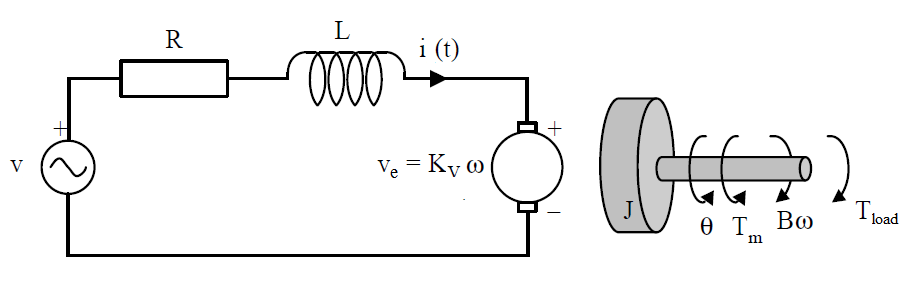
\includegraphics[width=0.65\textwidth]{images/motor_circuit.png}
  \caption{วงจรสมมูลของ Armature มอเตอร์กระแสตรง}
  \label{fig:motor_circuit}
\end{figure}

แรงดันย้อนกลับมีความสัมพันธ์กับความเร็วเชิงมุมของมอเตอร์ ($\omega_m$) ดังนี้

\begin{equation}
  e_b(t) = K_b\, \omega_m(t)
  \label{eq:bemf}
\end{equation}

โดยที่ $K_b$ คือค่าคงที่ Back-EMF (V$\cdot$s/rad)

\paragraph{ระบบกล (Mechanical Subsystem)}

แรงบิดที่มอเตอร์ผลิตได้สัมพันธ์กับกระแส Armature ดังนี้

\begin{equation}
  \tau_m(t) = K_t\, i_a(t)
  \label{eq:torque_motor}
\end{equation}

โดยที่ $K_t$ คือค่าคงที่แรงบิด (N$\cdot$m/A)

\paragraph{ชุดทดรอบ 2 ชั้น}

ระบบใช้ชุดทดรอบแบบ 2 ชั้น ได้แก่ Planetary Gearbox อัตราทดรอบ
$N_g = 24$ และ Belt Drive ที่มี Driver Pulley 24 teeth และ Driven Pulley 70 teeth
ให้อัตราทดรอบ $N_b = 70/24 = 2.917$ อัตราทดรอบรวมคือ

\begin{equation}
  N_{total} = N_g \times N_b = 24 \times \frac{70}{24} = 70
  \label{eq:gear_ratio}
\end{equation}

ความสัมพันธ์ระหว่างความเร็วเชิงมุมและแรงบิดที่ด้าน Output shaft
($\omega_{arm}$, $\tau_{out}$) กับด้าน Motor ($\omega_m$, $\tau_m$) คือ

\begin{equation}
  \omega_{arm}(t) = \frac{\omega_m(t)}{N_{total}}
  \label{eq:omega_arm}
\end{equation}

\begin{equation}
  \tau_{out}(t) = \eta\, N_{total}\, \tau_m(t)
  \label{eq:tau_out}
\end{equation}

โดยที่ $\eta$ คือประสิทธิภาพรวมของชุดทดรอบ

นำ \cref{eq:torque_motor} และ \cref{eq:tau_out} ไปใช้กับ
Newton's Second Law ที่ Output shaft

\begin{equation}
  J\, \frac{d\omega_{arm}(t)}{dt} = \tau_{out}(t) - b\, \omega_{arm}(t)
  \label{eq:newton}
\end{equation}

\begin{equation}
  J\, \frac{d\omega_{arm}(t)}{dt} = \eta\, N_{total}\, K_t\, i_a(t) - b\, \omega_{arm}(t)
  \label{eq:newton_expand}
\end{equation}

โดยที่ $J$ คือโมเมนต์ความเฉื่อยรวมของ Arm, Gripper และ Connection Rod
(kg$\cdot$m$^2$) และ $b$ คือสัมประสิทธิ์การหน่วงแบบ Viscous (N$\cdot$m$\cdot$s/rad)

\paragraph{Block Diagram ของระบบ}

Block Diagram ของแบบจำลองระบบมอเตอร์ที่สร้างใน Simulink
แสดงดัง\cref{fig:motor_block} ซึ่งประกอบด้วย Electrical Loop
ที่ป้อนกลับด้วย Back-EMF และ Mechanical Loop
ที่ป้อนกลับด้วย Viscous Damping

\begin{figure}[H]
  \centering
  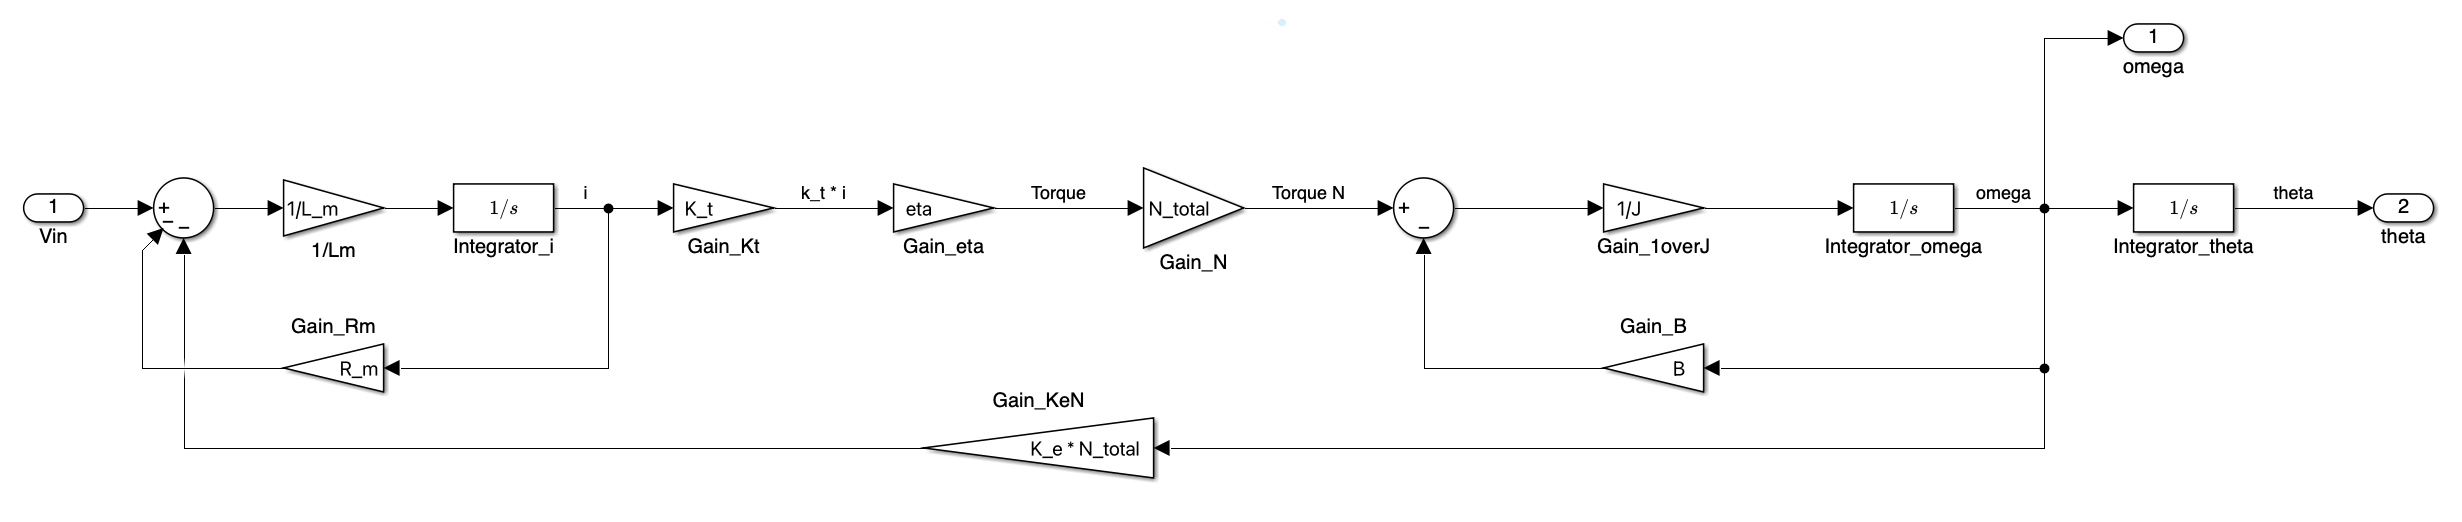
\includegraphics[width=0.92\textwidth]{images/simulink_motor_model.png}
  \caption{Block Diagram ของระบบมอเตอร์กระแสตรงพร้อมชุดทดรอบใน Simulink}
  \label{fig:motor_block}
\end{figure}

\paragraph{Transfer Function}

แปลง \cref{eq:kvl,eq:bemf,eq:newton_expand} เป็น Laplace domain
โดยสมมติเงื่อนไขเริ่มต้นเป็นศูนย์

\begin{align}
  V_{in}(s) &= (R_a + L_a s)\, I_a(s) + K_b\, N_{total}\, \Omega_{arm}(s)
  \label{eq:lap_elec} \\
  (Js + b)\, \Omega_{arm}(s) &= \eta\, N_{total}\, K_t\, I_a(s)
  \label{eq:lap_mech}
\end{align}

จาก \cref{eq:lap_mech} แทน $I_a(s)$ ลงใน \cref{eq:lap_elec}
แล้วจัดรูปได้ Velocity Transfer Function ดังนี้

\begin{equation}
  G_{vel}(s) = \frac{\Omega_{arm}(s)}{V_{in}(s)}
             = \frac{\eta K_t N_{total} / (L_a J)}
                    {s^2 + \left(\dfrac{R_a}{L_a} + \dfrac{b}{J}\right)s
                         + \dfrac{R_a b + K_b K_t N_{total}^2}{L_a J}}
  \label{eq:Gvel}
\end{equation}

สำหรับ Position Transfer Function เพิ่ม Integrator เนื่องจาก
$\Theta_{arm}(s) = \Omega_{arm}(s)/s$

\begin{equation}
  G_{pos}(s) = \frac{\Theta_{arm}(s)}{V_{in}(s)}
             = \frac{\eta K_t N_{total} / (L_a J)}
                    {s\left[s^2 + \left(\dfrac{R_a}{L_a} + \dfrac{b}{J}\right)s
                         + \dfrac{R_a b + K_b K_t N_{total}^2}{L_a J}\right]}
  \label{eq:Gpos}
\end{equation}

แทนค่าตัวเลขจาก System Identification

\begin{align}
  K_{num} &= \frac{\eta K_t N_{total}}{L_a J}
           = \frac{0.836 \times 0.04065 \times 70}{0.001448 \times 0.728}
           = \frac{2.376}{0.001054} = 2254 \notag \\
  a_1     &= \frac{R_a}{L_a} + \frac{b}{J}
           = \frac{1.453}{0.001448} + \frac{0.193}{0.728}
           = 1003.5 + 0.265 = 1003.8 \notag \\
  a_0     &= \frac{R_a b + K_b K_t N_{total}^2}{L_a J} \notag \\
           &= \frac{(1.453)(0.193) + (0.04165)(0.04065)(70)^2}{(0.001448)(0.728)} \notag \\
           &= \frac{0.280 + 8.297}{0.001054} = 8136 \notag
\end{align}

ดังนั้น Transfer Function เชิงตัวเลขคือ

\begin{equation}
  G_{vel}(s) = \frac{2254}{s^2 + 1003.8\,s + 8136}
  \label{eq:Gvel_num}
\end{equation}

\begin{equation}
  G_{pos}(s) = \frac{2254}{s\left(s^2 + 1003.8\,s + 8136\right)}
  \label{eq:Gpos_num}
\end{equation}

% ------------------------------------------------------------
\subsubsection{การทำ System Identification}
% ------------------------------------------------------------

\paragraph{พารามิเตอร์ที่วัดโดยตรง: Locked Rotor Test}

ค่า $R_a$ และ $L_a$ วัดด้วย Locked Rotor Test โดยจ่ายแรงดัน Step
ผ่าน Shunt Resistor $R_{sh} = 0.1\,\Omega$ แล้ววัดแรงดันตกคร่อม Shunt
ด้วย Oscilloscope ดังแสดงใน\cref{fig:locked_rotor_scope}
เพื่อหาค่า $V_{max}$ และค่าคงเวลา $\tau$ แล้วคำนวณด้วยสูตร

\paragraph{การเลือกค่า $R_{sh}$}

การเลือกค่า $R_{sh} = 0.1\,\Omega$ มาจากเงื่อนไข 2 ข้อดังนี้

\textbf{เงื่อนไขที่ 1: ไม่รบกวนวงจร}
ค่า $R_{sh}$ ต้องมีขนาดเล็กเมื่อเทียบกับ $R_a$ เพื่อไม่ให้กระทบต่อพฤติกรรมของวงจร
โดยกำหนดค่าคงที่ $k = 0.1$ ดังนี้

\begin{equation}
  \frac{R_{sh}}{R_a} < k \implies R_{sh} < 0.1 \times 1.453 = 0.1453\,\Omega
  \label{eq:rsh_condition1}
\end{equation}

\textbf{เงื่อนไขที่ 2: ทนกำลังไฟได้}
ประมาณกระแส Stall จากแรงดันสูงสุดและค่า $R_a$ ที่วัดได้

\begin{equation}
  I_{stall} \approx \frac{V_{in}}{R_a} = \frac{24}{1.453} \approx 16.5\,\text{A}
  \label{eq:i_stall}
\end{equation}

กำลังที่ $R_{sh}$ ต้องทนได้คือ

\begin{equation}
  P_{sh} = I_{stall}^2 \cdot R_{sh} = (16.5)^2 \times 0.1 \approx 27.2\,\text{W}
  \label{eq:p_sh}
\end{equation}

จากทั้งสองเงื่อนไข จึงเลือก $R_{sh} = 0.1\,\Omega$ 
ซึ่งน้อยกว่าขีดจำกัด $0.1453\,\Omega$ และต้องใช้ตัวต้านทานที่ทนกำลังได้อย่างน้อย $30\,\text{W}$

\paragraph{ที่มาของสูตร}

ขณะ Locked Rotor แกนมอเตอร์หยุดนิ่ง ทำให้ $\omega_m = 0$ 
และ Back-EMF หายไป $e_b = K_b\,\omega_m = 0$ วงจรจึงเหลือเพียง

\begin{equation}
  V_{in} = (R_a + R_{sh})\,i(t) + L_a\,\frac{di(t)}{dt}
  \label{eq:locked_rotor_circuit}
\end{equation}

\textbf{การหา $R_a$:}
ที่ Steady State กระแสนิ่ง $\frac{di}{dt} = 0$ และวัด $V_{sh,ss}$ ได้จาก Oscilloscope
ดังนั้น $i_{ss} = V_{sh,ss}/R_{sh}$ แทนกลับได้

\begin{equation}
  R_a = R_{sh}\left(\frac{V_{in}}{V_{sh,ss}} - 1\right)
  \label{eq:Ra_derive}
\end{equation}

\textbf{การหา $L_a$:}
Solution ของวงจร RL คือ $i(t) = i_{ss}(1 - e^{-t/\tau})$ 
โดยที่ $\tau = L_a/(R_a + R_{sh})$ จัดรูปได้

\begin{equation}
  L_a = \tau\,(R_a + R_{sh}) = R_{sh}\left(\tau\,\frac{V_{in}}{V_{sh,ss}}\right)
  \label{eq:La_derive}
\end{equation}

\begin{equation}
  R_a = R_{sh}\left(\frac{V_{in}}{V_{sh}} - 1\right), \qquad
  L_a = R_{sh}\left(\tau\,\frac{V_{in}}{V_{sh}}\right)
  \label{eq:locked_rotor}
\end{equation}

โดยที่ $V_{sh}$ คือแรงดันตกคร่อม Shunt ที่ Steady State

\begin{figure}[H]
  \centering
  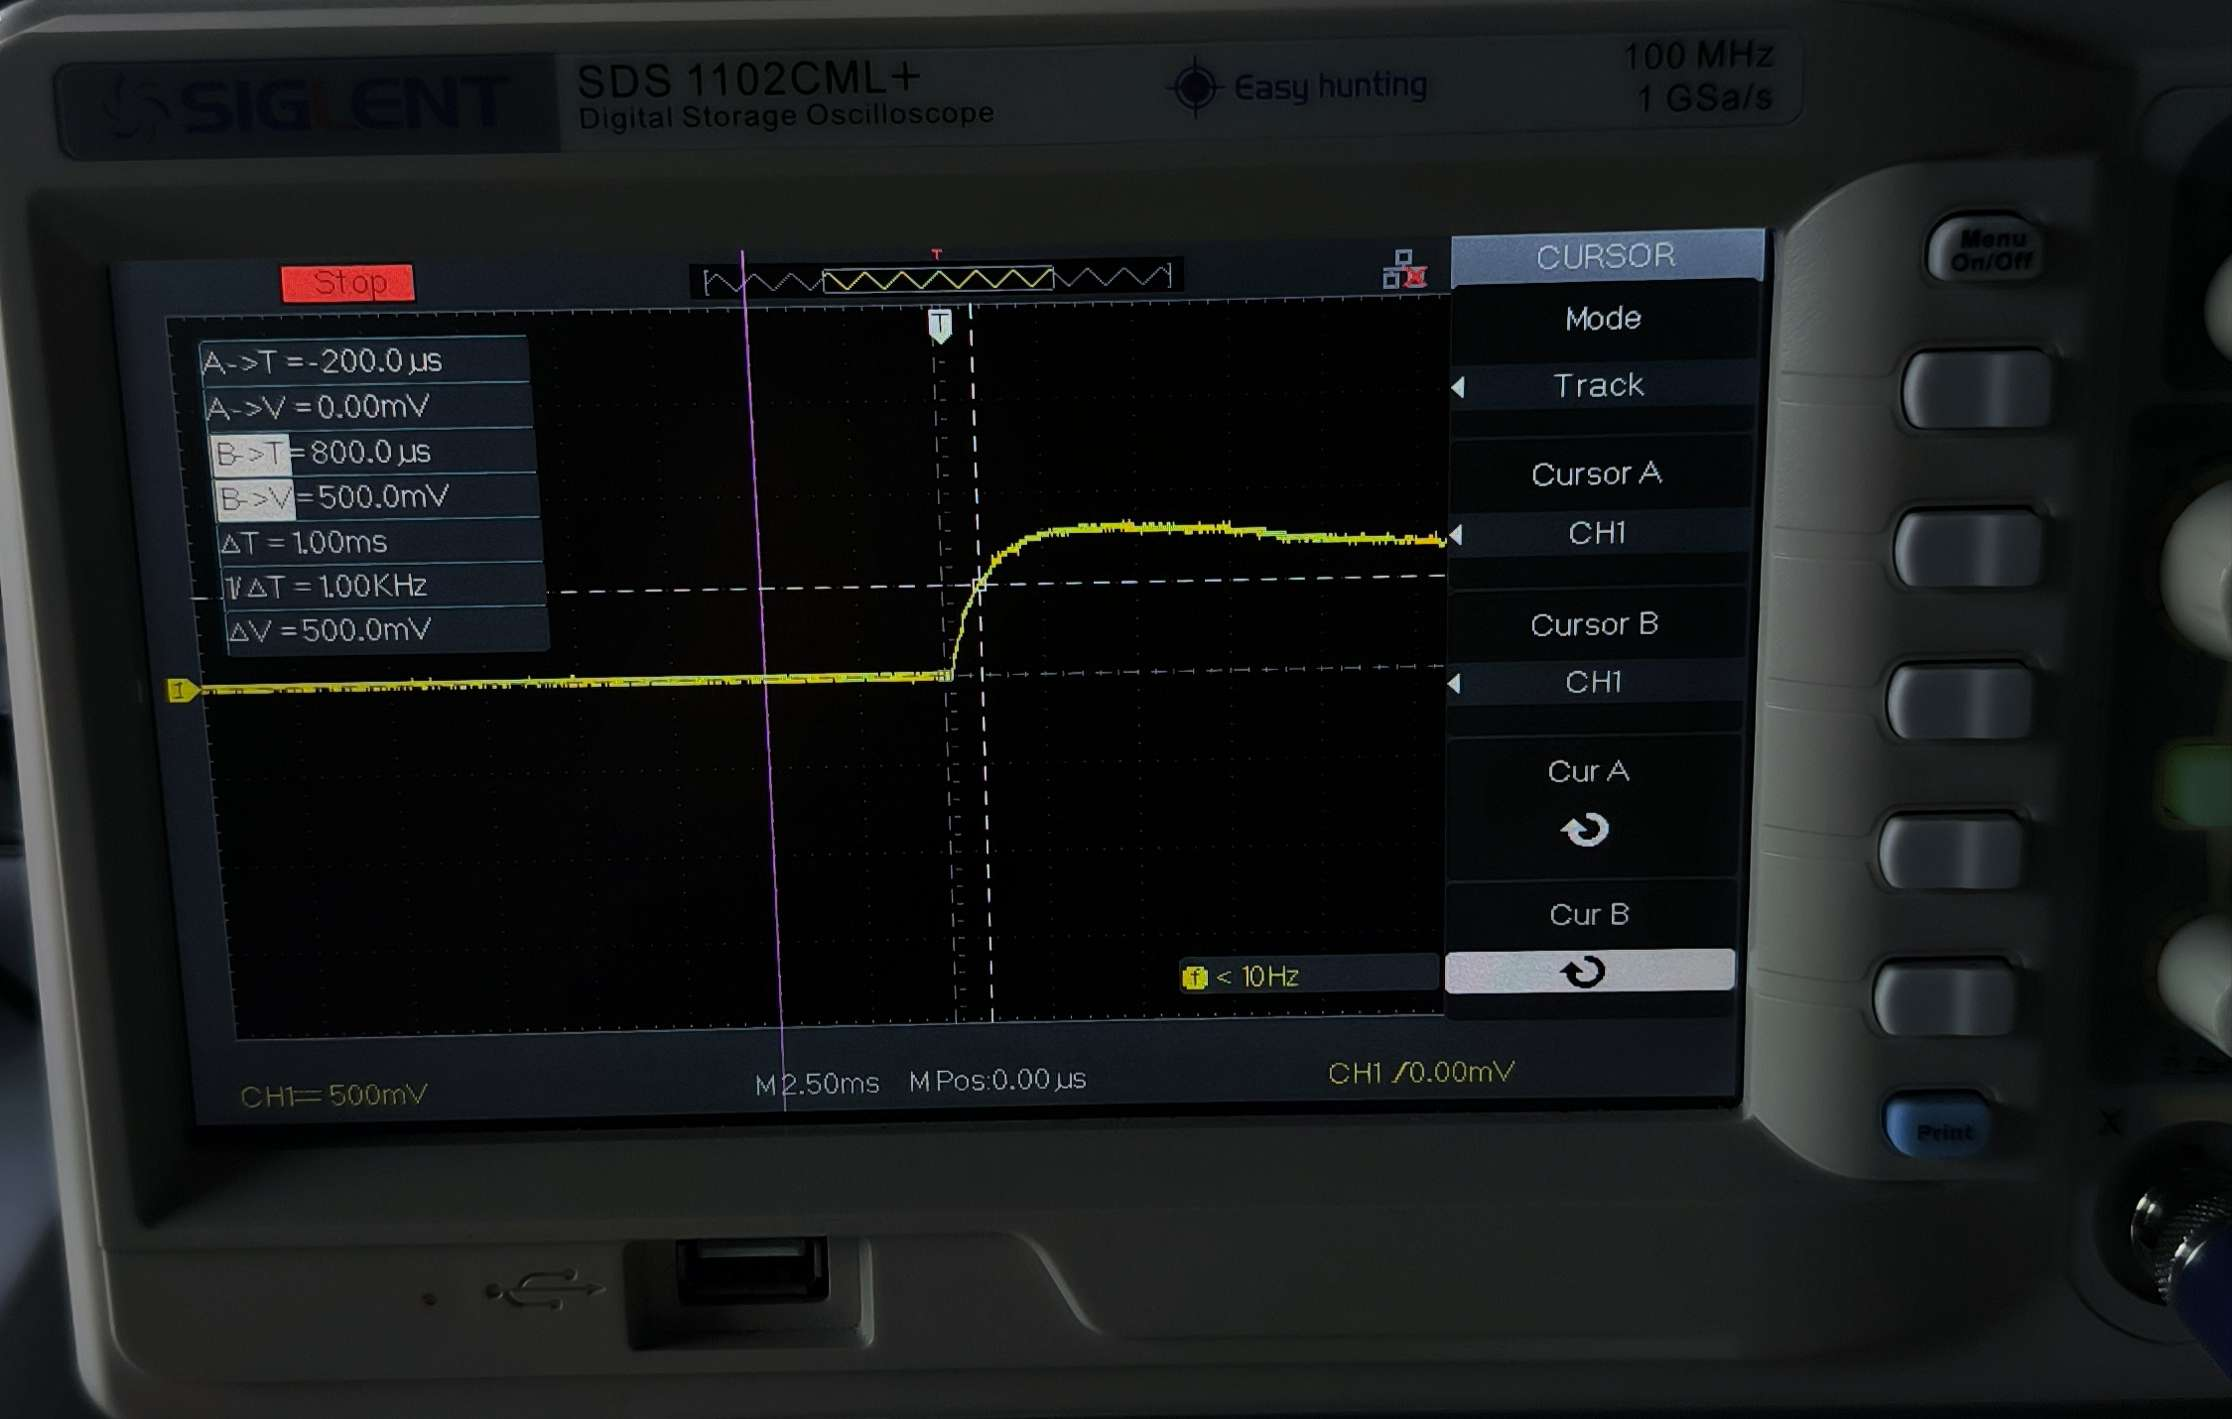
\includegraphics[width=0.70\textwidth]{images/locked_rotor_scope.png}
  \caption{Oscilloscope Waveform จาก Locked Rotor Test แสดง $V_{max}$ และ $\tau$}
  \label{fig:locked_rotor_scope}
\end{figure}

\paragraph{การเลือกแรงดันทดสอบ}

ทดสอบที่แรงดัน 3 ระดับ ได้แก่ $V_{in} = 6$, $9$ และ $12$\,V 
เพื่อตรวจสอบความสม่ำเสมอของค่าที่วัดได้ในแต่ละระดับ
ผลสรุปแสดงในตารางที่~\ref{tab:locked_rotor_all}

\begin{table}[H]
  \centering
  \caption{เปรียบเทียบผลการวัด $R_a$ และ $L_a$ จาก Locked Rotor Test ทั้ง 3 แรงดัน}
  \label{tab:locked_rotor_all}
  \begin{tabular}{ccccc}
    \toprule
    $V_{in}$ (V) & $\bar{R}_a$ ($\Omega$) & $\sigma_{R_a}$ ($\Omega$) 
                 & $\bar{L}_a$ (H)        & $\sigma_{L_a}$ (H) \\
    \midrule
    6  & 1.7300 & 0.0374 & 0.001490 & 0.000062 \\
    9  & 1.5398 & 0.0604 & 0.001473 & 0.000095 \\
    12 & 1.4534 & 0.0523 & 0.001448 & 0.000055 \\
    \bottomrule
  \end{tabular}
\end{table}

จากตารางพบว่าค่า $R_a$ มีแนวโน้มลดลงเมื่อแรงดันเพิ่มขึ้น 
ซึ่งเป็นผลจากสองปัจจัยหลัก ได้แก่
\begin{itemize}
  \item \textbf{Contact Resistance:} ที่แรงดันต่ำ กระแสที่ไหลผ่านน้อย
        ทำให้ความต้านทานสัมผัสของ Brush และขั้วต่อมีนัยสำคัญมากขึ้น
        เมื่อแรงดันสูงขึ้น สัดส่วนของ Contact Resistance ต่อ $R_a$ รวมลดลง
  \item \textbf{Signal-to-Noise Ratio:} ที่ $V_{in} = 6$\,V 
        แรงดันตกคร่อม Shunt $V_{sh}$ มีค่าต่ำ ทำให้ Noise 
        มีผลต่อการอ่านค่ามากกว่า ส่งผลให้ค่าที่วัดได้มี Error สูงกว่า
\end{itemize}

จึงเลือกใช้ผลจาก $V_{in} = 12$\,V เป็นค่าอ้างอิง เนื่องจากสองเหตุผล ได้แก่
\begin{enumerate}
  \item ใกล้เคียงกับแรงดันใช้งานจริง $24$\,V มากที่สุดในบรรดาแรงดันที่ทดสอบ
        ทำให้สภาวะของ Brush Contact ใกล้เคียงกับการทำงานจริงมากที่สุด
  \item ไม่ทดสอบที่ $24$\,V เนื่องจากขณะ Locked Rotor 
        กระแส Stall $I_{stall} \approx V_{in}/R_a = 24/1.453 \approx 16.5$\,A 
        จะทำให้ $R_{sh}$ รับกำลัง $P_{sh} = I_{stall}^2 \cdot R_{sh} 
        = (16.5)^2 \times 0.1 \approx 27.2$\,W ซึ่งเกินพิกัดและอาจเป็นอันตรายได้
\end{enumerate}

เลือกใช้ค่าทดสอบที่ $V_{in} = 12$\,V จำนวน 3 ครั้ง ผลการวัดแสดงใน\cref{tab:locked_rotor}

\begin{table}[H]
  \centering
  \caption{ผลการวัด $R_a$ และ $L_a$ จาก Locked Rotor Test ที่ 12\,V}
  \label{tab:locked_rotor}
  \begin{tabular}{lcccc}
    \toprule
    Run & $V_{max}$ (V) & $\tau$ (s) & $R_a$ ($\Omega$) & $L_a$ (H) \\
    \midrule
    1 & 0.740 & 0.00090 & 1.52162 & 0.001459 \\
    2 & 0.780 & 0.00090 & 1.43846 & 0.001385 \\
    3 & 0.800 & 0.00100 & 1.40000 & 0.001500 \\
    \midrule
    \textbf{Mean} & & & \textbf{1.45336} & \textbf{0.001448} \\
    \bottomrule
  \end{tabular}
\end{table}

ค่าเฉลี่ยที่ได้จากการทดสอบ 3 ครั้ง คือ $R_a = 1.453\,\Omega$ และ $L_a = 1.448\,\text{mH}$
ซึ่งจะใช้เป็นค่าอ้างอิงในการสร้างแบบจำลองและออกแบบระบบควบคุมในหัวข้อถัดไป

\paragraph{การเลือกสัญญาณ Excitation}

เลือกใช้ Chirp Signal เป็น Excitation เนื่องจากเป็นสัญญาณ Sine Wave 
ที่ความถี่เพิ่มขึ้นเรื่อย ๆ ตามเวลา (Frequency Sweep) 
ทำให้สามารถ Excite พฤติกรรมของมอเตอร์ได้ครอบคลุมทั้งย่านความถี่ต่ำ 
(Slow Dynamics เช่น Inertia และ Viscous Damping) 
และย่านความถี่สูง (Fast Dynamics เช่น Friction) ภายใน Input เดียว
สัญญาณอื่น เช่น Step หรือ Impulse มีพลังงานกระจุกตัวอยู่ที่ความถี่เดียว
จึงให้ข้อมูล Frequency Content ที่ไม่ครอบคลุมเท่า

\paragraph{การเลือกย่านความถี่ 0.1--2.0\,Hz}

ขอบล่าง $f_{min} = 0.1$\,Hz เลือกเพื่อให้ครอบคลุม Slow Dynamics 
ของระบบ โดยเฉพาะ Inertia $J$ ที่มีผลเด่นชัดที่ความถี่ต่ำมาก

ขอบบน $f_{max} = 2.0$\,Hz กำหนดจาก Mechanical Bandwidth ของระบบ
ซึ่งประมาณได้จากพารามิเตอร์ที่วัดได้ดังนี้

\begin{equation}
  f_{mech} = \frac{1}{2\pi}\sqrt{\frac{R_a b + K_b K_t N^2}{L_a J}}
           = \frac{1}{2\pi}\sqrt{8136}
           \approx 14.4\,\text{Hz}
  \label{eq:f_mech}
\end{equation}

ค่า $f_{max} = 2.0$\,Hz คิดเป็นประมาณ 14\% ของ $f_{mech}$ 
ซึ่งอยู่ในย่านที่ระบบยังตามสัญญาณได้ดี 
และไม่สูงจนมอเตอร์ไม่สามารถตอบสนองได้ทัน
นอกจากนี้ยังเลือกทดสอบ 3 กลุ่มความถี่ ได้แก่ 
0.1--0.5\,Hz, 0.1--1.0\,Hz และ 0.1--2.0\,Hz 
เพื่อตรวจสอบความสม่ำเสมอของผลการ Estimate ในแต่ละย่านความถี่

\paragraph{การ Preprocess ข้อมูล}

ข้อมูลดิบจาก Hardware กรองด้วย Butterworth Low-pass Filter Order 4
ที่ Cutoff Frequency $f_c = 10$\,Hz โดยเลือกจากเงื่อนไข

\begin{equation}
  f_c = 5 \times f_{max} = 5 \times 2.0 = 10\,\text{Hz}
  \label{eq:fc}
\end{equation}

เพื่อให้สัญญาณ Chirp ทุกความถี่ผ่านได้เต็มที่ 
ในขณะที่ลด Noise ความถี่สูงจาก Encoder และ Electrical Noise ออก
เลือก Butterworth เนื่องจากมี Flat Passband 
ไม่บิดเบือน Amplitude ของสัญญาณในย่านที่สนใจ
และ Order 4 ให้ Attenuation ที่ $10 f_c = 100$\,Hz สูงถึง

\begin{equation}
  A = -20 \times 4 \times \log_{10}\!\left(\frac{100}{10}\right) = -80\,\text{dB}
  \label{eq:attenuation}
\end{equation}

ซึ่งเพียงพอในการกำจัด Noise ความถี่สูงออกจากสัญญาณ
ใช้ \texttt{filtfilt} แทน \texttt{filter} ธรรมดา 
เพื่อให้ Phase Shift เป็นศูนย์ตลอดทุกความถี่
เนื่องจากหาก Phase Shift ไม่เป็นศูนย์ 
จะทำให้ความสัมพันธ์ระหว่าง $V_{in}$ และ $\omega_{arm}$ในเชิงเวลาคลาดเคลื่อน
ส่งผลให้ Parameter Estimator ได้ค่าพารามิเตอร์ที่ผิดพลาดได้

\textbf{ผลการตรวจสอบความถูกต้องของแบบจำลอง (Model Validation)}

การตรวจสอบความถูกต้องของแบบจำลองกระทำโดยนำแบบจำลองไปจำลองการทำงานเปรียบเทียบกับข้อมูลจริงจาก Hardware ในเงื่อนไขต่าง ๆ (Cross-Validation) เพื่อคำนวณ Fit Score และ NRMSE โดยรายละเอียดผลการตรวจสอบโดยละเอียดแสดงใน\cref{subsec:model_validation_results}

\begin{table}[H]
  \centering
  \caption{พารามิเตอร์ที่ได้จาก System Identification}
  \label{tab:sysid_params}
  \begin{tabular}{llccc}
    \toprule
    พารามิเตอร์ & สัญลักษณ์ & ค่า & หน่วย & วิธีการ \\
    \midrule
    Armature Resistance    & $R_a$  & 1.4534   & $\Omega$              & Locked Rotor Test \\
    Armature Inductance    & $L_a$  & 0.001448 & H                     & Locked Rotor Test \\
    Back-EMF Constant      & $K_b$  & 0.04165  & V$\cdot$s/rad         & Parameter Estimation \\
    Torque Constant        & $K_t$  & 0.04065  & N$\cdot$m/A           & Parameter Estimation \\
    Viscous Damping        & $b$    & 0.19279  & N$\cdot$m$\cdot$s/rad & Parameter Estimation \\
    Moment of Inertia      & $J$    & 0.72762  & kg$\cdot$m$^2$        & Parameter Estimation \\
    Gear Ratio (Planetary) & $N_g$  & 24       & --                    & Datasheet \\
    Belt Drive Ratio       & $N_b$  & 2.917    & --                    & การออกแบบ \\
    Total Gear Ratio       & $N$    & 70       & --                    & $N_g \times N_b$ \\
    Efficiency             & $\eta$ & 0.836    & --                    & Parameter Estimation \\
    \bottomrule
  \end{tabular}
\end{table}

% ------------------------------------------------------------
\subsubsection{การออกแบบตัวควบคุม PID ด้วย Root Locus}
% ------------------------------------------------------------

\paragraph{โครงสร้างระบบควบคุม}

ระบบควบคุมใช้โครงสร้าง Cascade PID Control
ซึ่งประกอบด้วย 2 Loop ซ้อนกัน ดังแสดงใน\cref{fig:cascade_block}
โดย Velocity Inner Loop ทำหน้าที่ควบคุมความเร็วเชิงมุม $\omega_{arm}$
และ Position Outer Loop ทำหน้าที่ควบคุมตำแหน่ง $\theta_{arm}$
พร้อมด้วย Velocity Feedforward และ Acceleration Feedforward
เพื่อลด Tracking Error

\begin{figure}[H]
  \centering
  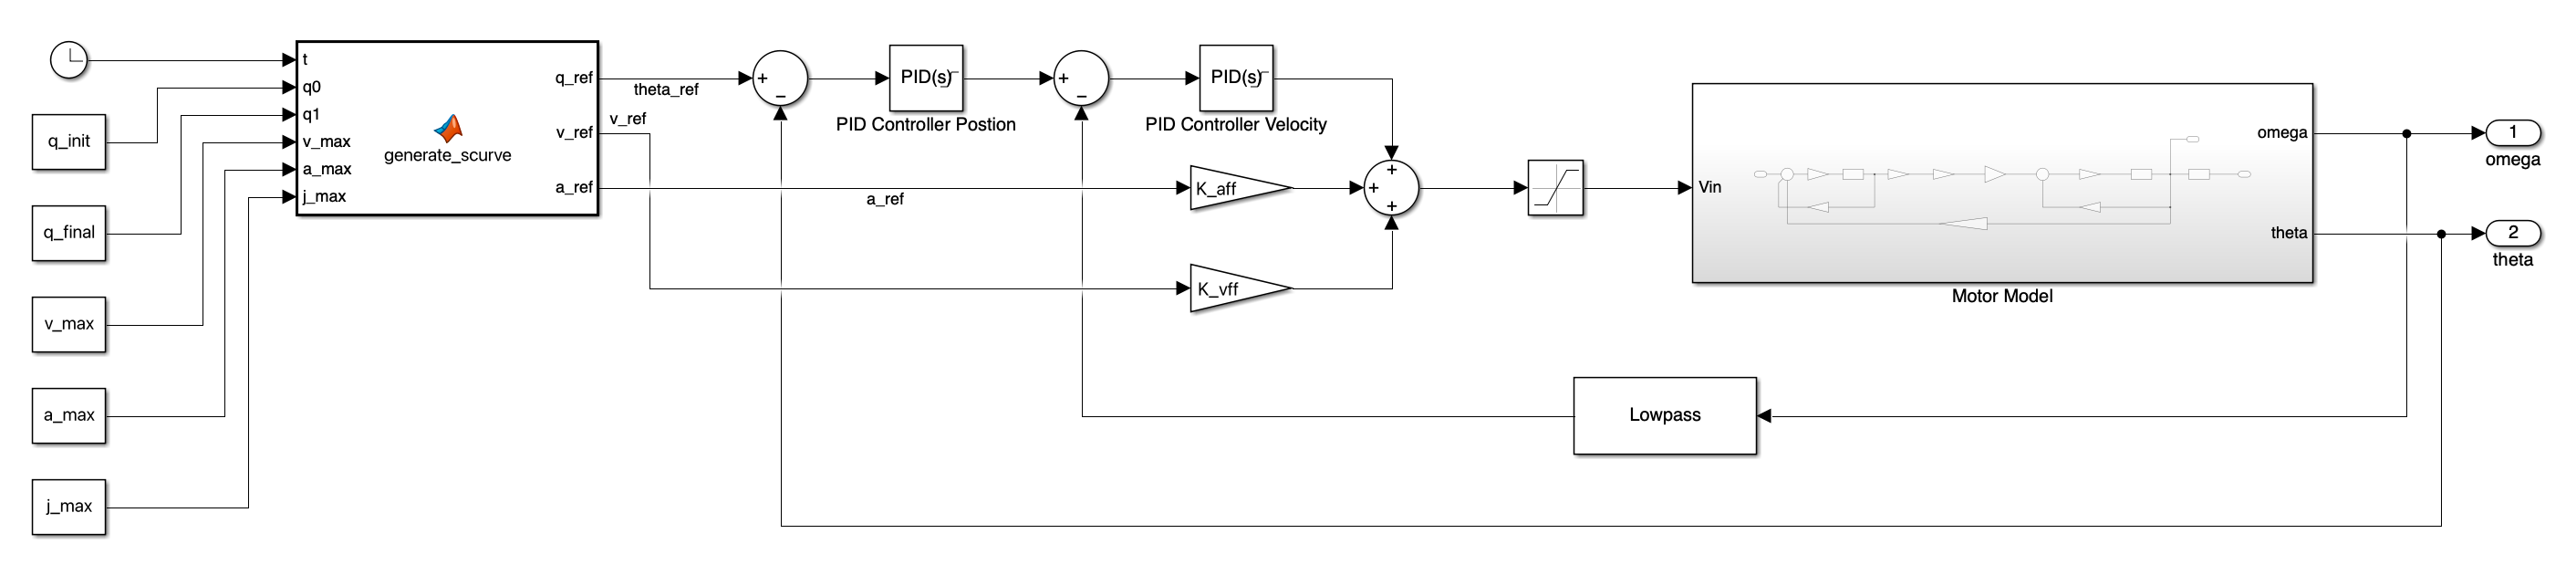
\includegraphics[width=0.95\textwidth]{images/simulink_cascade.png}
  \caption{Block Diagram ของ Cascade PID Control พร้อม Feedforward}
  \label{fig:cascade_block}
\end{figure}

\paragraph{ข้อกำหนดการออกแบบ}

\begin{table}[H]
  \centering
  \caption{ข้อกำหนดของระบบควบคุม}
  \label{tab:ctrl_req}
  \begin{tabular}{llcc}
    \toprule
    ข้อกำหนด & สัญลักษณ์ & ค่า & รหัส \\
    \midrule
    Settling Time & $t_s$  & $\leq 0.5$ s & P5 \\
    Overshoot     & $\%OS$ & $\leq 1\%$   & P6 \\
    \bottomrule
  \end{tabular}
\end{table}

\paragraph{การวิเคราะห์ Frequency Response ของ Plant}

ก่อนการออกแบบ Controller จำเป็นต้องวิเคราะห์ Frequency Response 
ของ Plant ก่อน เพื่อทำความเข้าใจพฤติกรรมของระบบในแต่ละย่านความถี่
โดยใช้ Bode Plot ซึ่งประกอบด้วยกราฟ 2 ส่วน ได้แก่

\begin{itemize}
  \item \textbf{Magnitude (dB):} แสดงอัตราส่วนขนาดระหว่าง Output และ Input 
        ที่แต่ละความถี่ เช่น $-20$\,dB หมายความว่า Output มีขนาดเล็กกว่า 
        Input อยู่ 10 เท่า ค่า 0\,dB หมายความว่า Output มีขนาดเท่ากับ Input พอดี
  \item \textbf{Phase (deg):} แสดงความล่าช้าของ Output เทียบกับ Input 
        ที่แต่ละความถี่ เช่น $-90°$ หมายความว่า Output ตามหลัง Input อยู่ 
        $\frac{1}{4}$ คาบของสัญญาณนั้น
\end{itemize}

\textbf{Velocity Plant และ Position Plant}

ระบบนี้ใช้ Plant 2 แบบขึ้นอยู่กับ Output ที่สนใจ ได้แก่

\begin{itemize}
  \item $G_{vel}(s)$: Input คือ $V_{in}$ และ Output คือ $\omega_{arm}$ 
        ใช้สำหรับออกแบบ Velocity Inner Loop
  \item $G_{pos}(s)$: Input คือ $V_{in}$ และ Output คือ $\theta_{arm}$ 
        ใช้สำหรับออกแบบ Position Outer Loop
\end{itemize}

ความสัมพันธ์ระหว่างทั้งสองคือ

\begin{equation}
  G_{pos}(s) = \frac{G_{vel}(s)}{s}
  \label{eq:gpos_gvel}
\end{equation}

การหาร $s$ เท่ากับการเพิ่ม Integrator หนึ่งตัว ส่งผลให้ Phase ของ 
$G_{pos}(s)$ ต่ำกว่า $G_{vel}(s)$ อยู่ $90°$ ตลอดทุกความถี่
ดังที่เห็นในรูปที่~\ref{fig:bode_plant} ว่า Phase ของ $G_{pos}(s)$ 
เริ่มต้นที่ $-90°$ แทนที่จะเริ่มที่ $0°$ เหมือน $G_{vel}(s)$

\textbf{การเลือก Damping Ratio $\zeta = 0.85$}

Damping Ratio $\zeta$ กำหนดจาก Overshoot Requirement ที่ระบุไว้ใน P6 
ว่า OS $\leq 1\%$ โดย Solve หาค่า $\zeta$ ขั้นต่ำที่ทำให้เงื่อนไขนี้สำเร็จ
จากสมการ Overshoot ของระบบ Second-Order

\begin{equation}
  \%OS = e^{-\pi\zeta/\sqrt{1-\zeta^2}} \times 100 \leq 1
  \label{eq:os_requirement}
\end{equation}

จัดรูปสมการโดยนำ Log ทั้งสองข้าง

\begin{equation}
  \frac{\pi\zeta}{\sqrt{1-\zeta^2}} \geq -\ln\!\left(\frac{1}{100}\right) 
  = \ln(100) = 4.605
  \label{eq:os_log}
\end{equation}

แก้สมการหา $\zeta$ ขั้นต่ำได้

\begin{equation}
  \zeta_{min} = \frac{4.605}{\sqrt{\pi^2 + 4.605^2}} 
              = \frac{4.605}{\sqrt{9.870 + 21.206}} 
              = \frac{4.605}{5.575} 
              \approx 0.826
  \label{eq:zeta_min}
\end{equation}

จึงเลือก $\zeta = 0.85$ ซึ่งสูงกว่าขีดจำกัด $\zeta_{min} = 0.826$ 
เพื่อให้มี Margin เพียงพอสำหรับความไม่แน่นอนของระบบจริง
และยืนยันได้ว่าได้ Overshoot จริงคือ

\begin{equation}
  \%OS = e^{-\pi(0.85)/\sqrt{1-0.85^2}} \times 100 
       = e^{-\pi(0.85)/0.527} \times 100 
       = 0.43\%
  \label{eq:os_verify}
\end{equation}

ซึ่งต่ำกว่าเกณฑ์ $1\%$ อย่างชัดเจน

\textbf{Phase Margin และความสำคัญต่อเสถียรภาพ}

จุดสำคัญที่ต้องอ่านจาก Bode Plot ก่อนออกแบบ Controller มีสองจุด ได้แก่

\begin{itemize}
  \item \textbf{Gain Crossover Frequency ($\omega_c$):} คือความถี่ที่ 
        Magnitude $= 0$\,dB หมายความว่าที่ความถี่นี้ Output มีขนาดเท่ากับ 
        Input พอดี $\omega_c$ บอกถึงความเร็วในการตอบสนองของระบบ 
        Closed-Loop ยิ่ง $\omega_c$ สูง ระบบยิ่งตอบสนองเร็ว
  \item \textbf{Phase Margin (PM):} คือระยะห่างระหว่าง Phase ที่ $\omega_c$ 
        กับ $-180°$ คำนวณได้จาก
        \begin{equation}
          PM = 180° + \angle G(j\omega_c)
          \label{eq:phase_margin}
        \end{equation}
        ยิ่ง PM สูง ระบบยิ่ง Stable และมี Overshoot น้อย 
        หาก PM ต่ำกว่า $0°$ ระบบจะ Oscillate ไม่หยุด
\end{itemize}

จากรูปที่~\ref{fig:bode_plant} พบว่า $G_{pos}(s)$ มีเส้นประแสดง 
$-135°$ (ซึ่งสอดคล้องกับ PM $= 45°$) และ $-180°$ ไว้เป็นเกณฑ์อ้างอิง
แสดงให้เห็นว่า Plant เปล่าๆ ยังไม่มี Phase Margin เพียงพอสำหรับ
ข้อกำหนด Overshoot $\leq 1\%$ จึงจำเป็นต้องออกแบบ Controller 
เพื่อชดเชย Phase ที่ขาดไป

\begin{figure}[H]
  \centering
  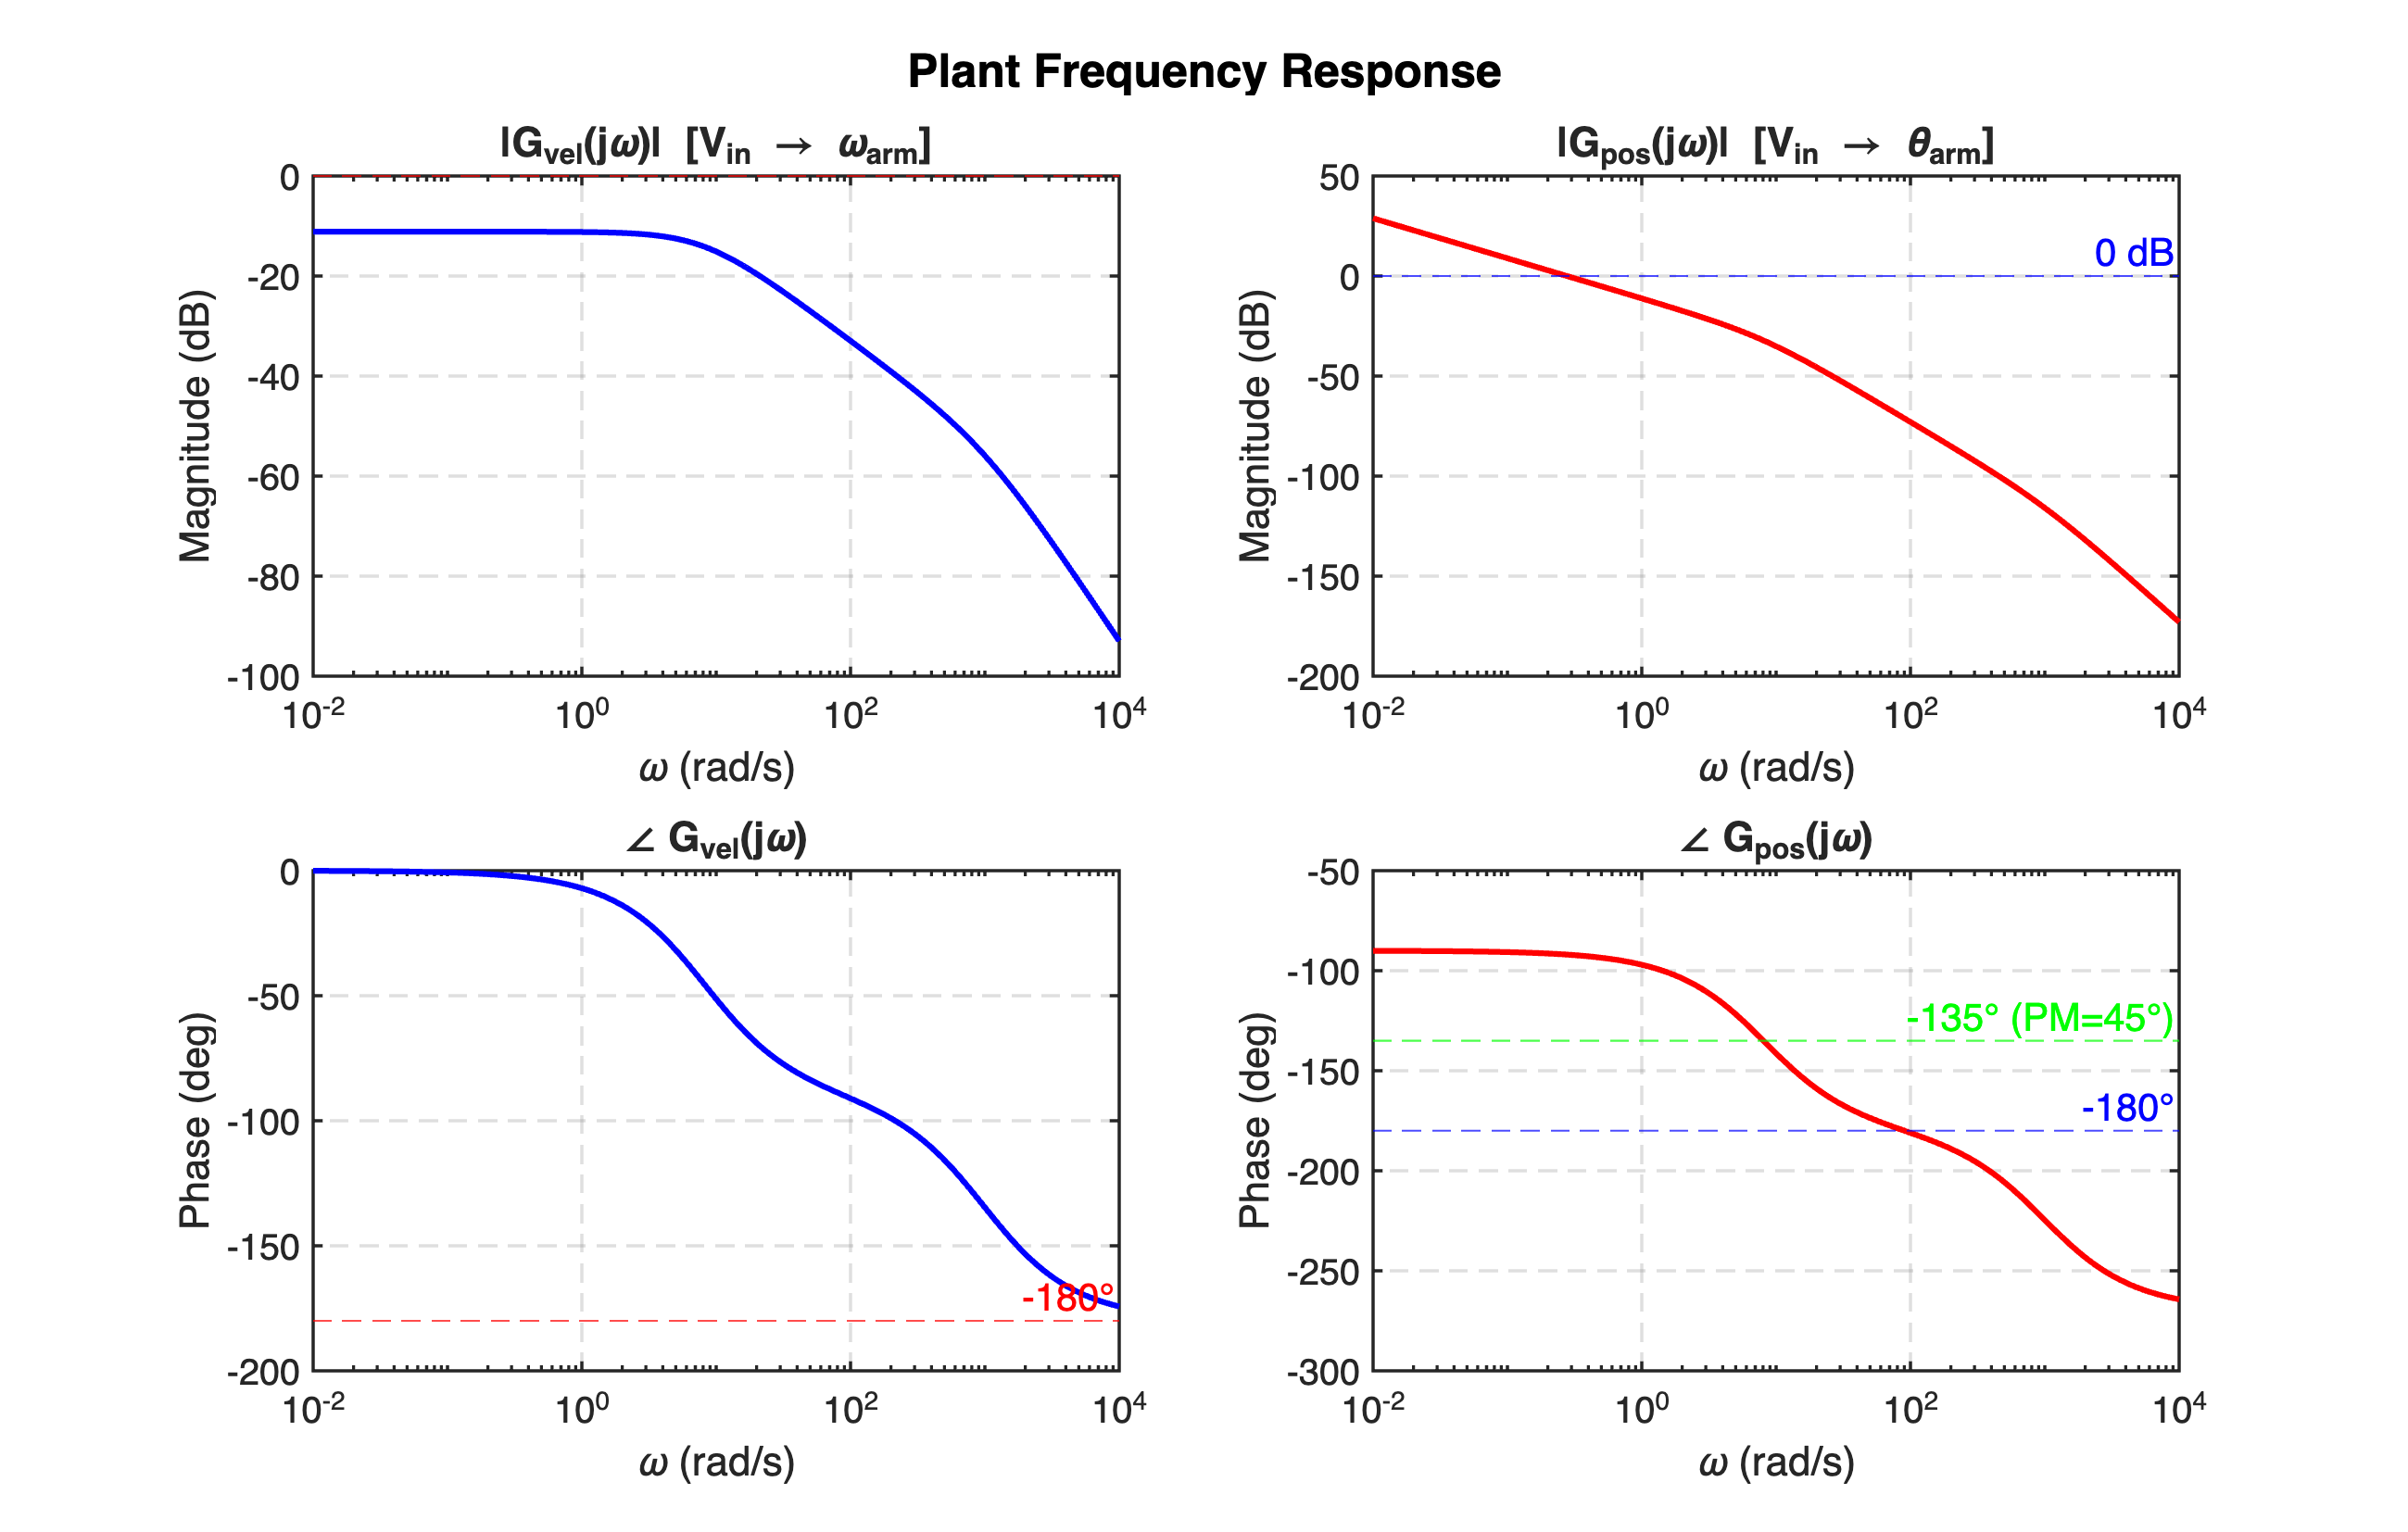
\includegraphics[width=0.88\textwidth]{images/bode_plant.png}
  \caption{Bode Plot ของ Velocity Plant $G_{vel}(s)$ และ Position Plant $G_{pos}(s)$}
  \label{fig:bode_plant}
\end{figure}

\paragraph{การออกแบบ Velocity Inner Loop}

\textbf{ทำไมต้องเร็วกว่า Position Loop 5 เท่า}

ระบบ Cascade Control ประกอบด้วย 2 Loop ซ้อนกัน โดย Velocity Inner Loop
ทำหน้าที่ควบคุมความเร็ว และ Position Outer Loop ทำหน้าที่ควบคุมตำแหน่ง
หลักการออกแบบ Cascade Control กำหนดให้ Inner Loop ต้องตอบสนองเร็วกว่า
Outer Loop อย่างน้อย 3--10 เท่า เพื่อให้ Outer Loop มองเห็น Inner Loop
เป็นเสมือน Ideal Follower ที่ตามคำสั่งได้ทันที
หากความเร็วของทั้งสอง Loop ใกล้เคียงกัน Loop ทั้งสองจะ Interact กัน
ทำให้ระบบไม่เสถียร จึงเลือก 5 เท่าเป็นค่ากลางที่ปลอดภัย

\begin{equation}
  \omega_{c,vel} \geq 5\,\omega_{c,pos} = 5 \times 9.41 = 47.1\,\text{rad/s}
  \quad \Rightarrow \quad
  \omega_{c,vel} = 47\,\text{rad/s}
\end{equation}

\textbf{ที่มา of Phase $-82.8°$ ที่ $\omega = 47$\,rad/s}

Transfer Function ของ Velocity Plant คือ

\begin{equation}
  G_{vel}(s) = \frac{2254}{s^2 + 1003.8\,s + 8136}
\end{equation}

แทน $s = j\omega = j47$ เพื่อหา Phase

\begin{equation}
  \begin{split}
    G_{vel}(j47) &= \frac{2254}{(j47)^2 + 1003.8(j47) + 8136} \\
                 &= \frac{2254}{(8136 - 47^2) + j(1003.8 \times 47)} \\
                 &= \frac{2254}{5927 + j47{,}179}
  \end{split}
  \label{eq:gvel_j47}
\end{equation}

Phase ของ $G_{vel}(j47)$ คือ Phase ของตัวส่วน ซึ่งเป็น Complex Number

\begin{equation}
  \angle G_{vel}(j47) = -\arctan\!\left(\frac{47{,}179}{5927}\right)
                      = -\arctan(7.960)
                      = -82.8°
  \label{eq:vel_phase}
\end{equation}

หมายความว่า Plant เปล่าๆ ที่ $\omega_c = 47$\,rad/s มี Phase อยู่ที่ $-82.8°$
ดังนั้น Phase Margin ของ Plant เปล่าๆ คือ $180° - 82.8° = 97.2°$
ซึ่งสูงกว่าเกณฑ์ $70°$ แต่ยังต้องใส่ PID เพื่อปรับ Gain ให้ถูกต้อง
โดยใช้ \texttt{pidtune} ของ MATLAB ออกแบบที่ $\omega_c = 47$\,rad/s
และ $PM = 70°$ ได้ Phase Margin จริง $79.2°$

\paragraph{การออกแบบ Position Outer Loop}

การเลือก Damping Ratio $\zeta = 0.85$ และการคำนวณที่เกี่ยวข้องเป็นไปตามเกณฑ์ที่ระบุไว้ก่อนหน้าเพื่อให้ได้ Overshoot $\leq 1\%$ และ Settling Time ตามข้อกำหนด

\textbf{การคำนวณ Crossover Frequency ของ Position Loop}

กำหนด $\omega_{c,pos}$ จาก Settling Time Requirement P5 ที่ระบุว่า
$t_s \leq 0.5$\,s โดยใช้ความสัมพันธ์ของระบบ Second-Order

\begin{equation}
  t_s \approx \frac{4}{\zeta\,\omega_{c,pos}}
  \quad \Rightarrow \quad
  \omega_{c,pos} = \frac{4}{\zeta\, t_s}
                = \frac{4}{0.85 \times 0.5}
                = 9.41\,\text{rad/s}
  \label{eq:pos_target}
\end{equation}

และกำหนด $PM_{pos} \geq 80°$ เพื่อให้ได้ Damping ที่สอดคล้องกับ
$\zeta = 0.85$ ในระบบ Closed-Loop จริง
โดยใช้ความสัมพันธ์ประมาณ $PM \approx 100\zeta = 85°$
แล้วเลือก $80°$ เป็นขีดจำกัดขั้นต่ำเพื่อให้มี Margin

Open-loop Bode Plot หลัง design แสดงดัง\cref{fig:bode_openloop}

\begin{figure}[H]
  \centering
  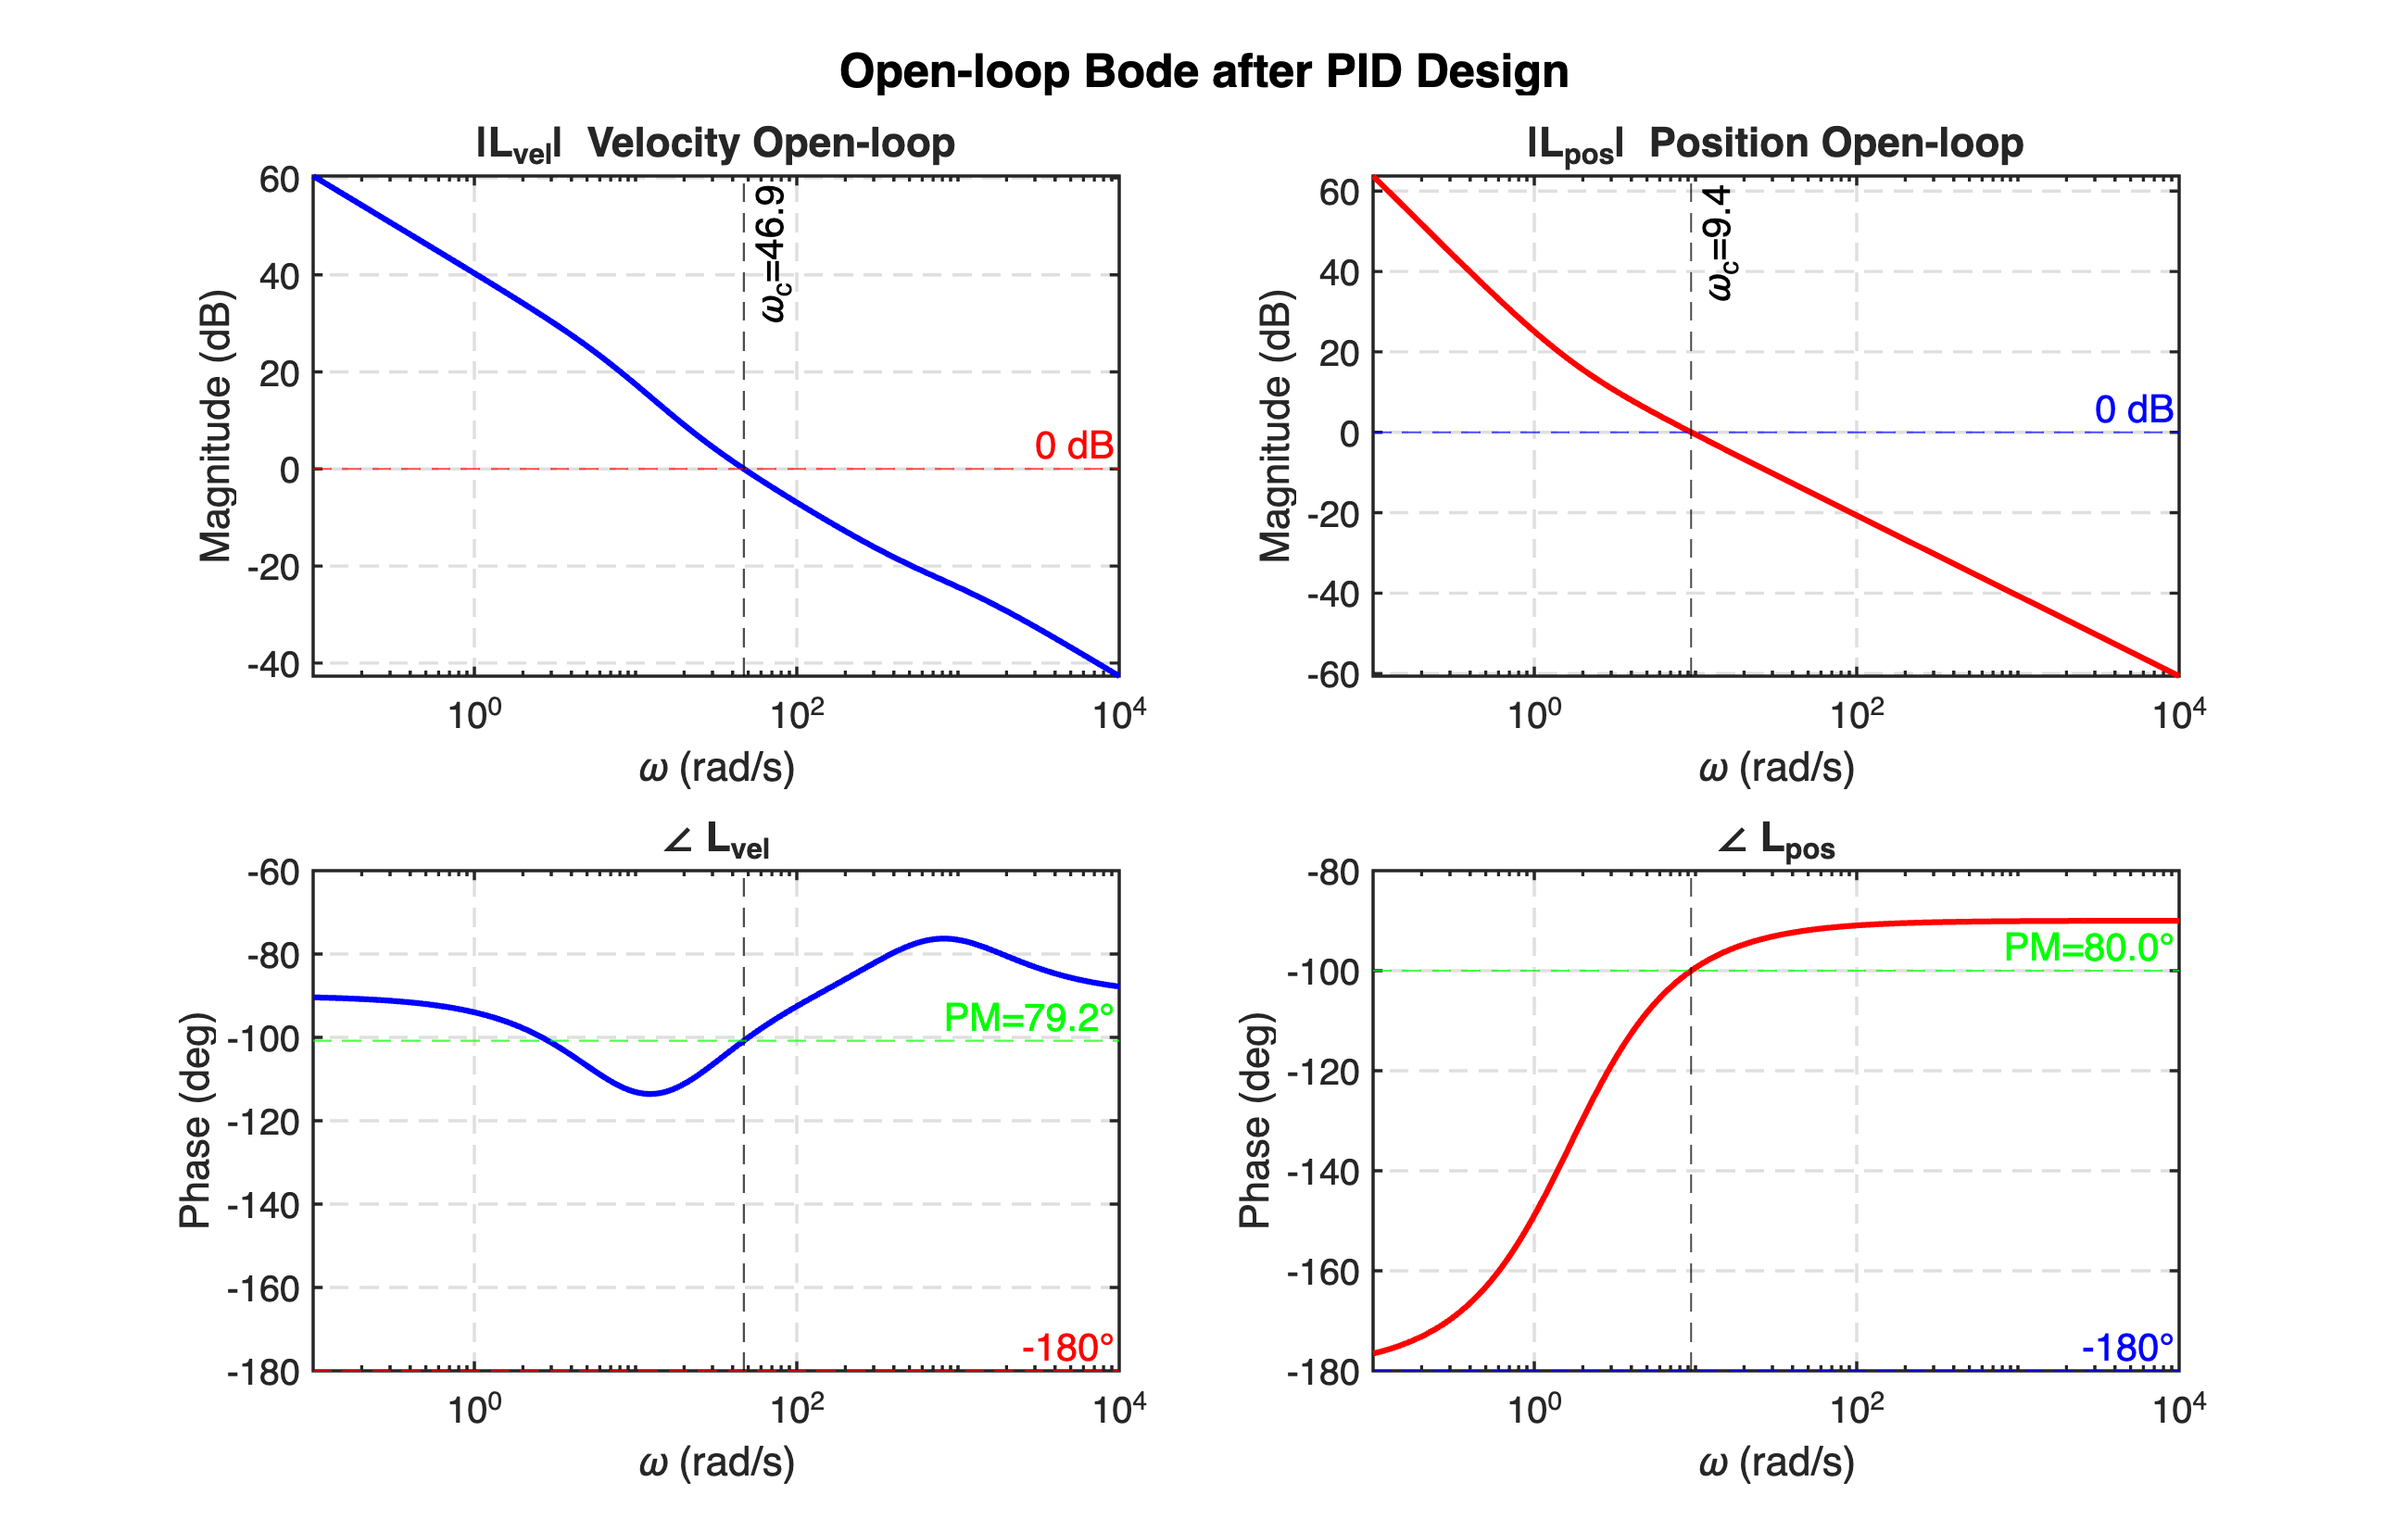
\includegraphics[width=0.88\textwidth]{images/bode_openloop.png}
  \caption{Open-loop Bode Plot ของ Velocity Loop และ Position Loop หลัง Design
           แสดง Crossover Frequency และ Phase Margin}
  \label{fig:bode_openloop}
\end{figure}

\paragraph{Feedforward Gains}

\textbf{ทำไมต้องมี Feedforward เพิ่มจาก PID}

PID Controller ทำงานแบบ Reactive คือรอให้เกิด Error ก่อนแล้วจึงแก้ไข
ในขณะที่ S-Curve Profile เปลี่ยน Reference ตลอดเวลา
ทำให้ PID มี Tracking Error สะสมตลอดช่วงการเคลื่อนที่
Feedforward แก้ปัญหานี้โดยคำนวณ Voltage ที่ต้องการล่วงหน้า
จาก Reference Velocity และ Acceleration โดยตรง
ทำให้ PID ต้องแก้ไขแค่ส่วนที่เหลือจาก Model Error เท่านั้น

\textbf{ที่มา of สูตร $K_{vff}$}

ที่ Steady State ความเร่งเป็นศูนย์ $\dot{\omega}_{arm} = 0$
สมการกลของระบบที่ Output Shaft คือ

\begin{equation}
  0 = \eta\, N\, K_t\, i_a - b\,\omega_{arm}
  \quad \Rightarrow \quad
  i_a = \frac{b\,\omega_{arm}}{\eta\, N\, K_t}
  \label{eq:ia_ss}
\end{equation}

แทนลงในสมการไฟฟ้าที่ Steady State ($\frac{di_a}{dt} = 0$)

\begin{equation}
  V_{in} = R_a\, i_a + K_b\, N\,\omega_{arm}
         = \frac{R_a\, b}{\eta\, N\, K_t}\,\omega_{arm} + K_b\, N\,\omega_{arm}
  \label{eq:vin_ss}
\end{equation}

ดังนั้น Velocity Feedforward Gain คือ

\begin{equation}
  \begin{split}
    K_{vff} &= \frac{V_{in}}{\omega_{arm}}
             = \frac{R_a\, b}{\eta\, N\, K_t} + K_b\, N \\
            &= \frac{1.453 \times 0.193}{0.04065 \times 0.836 \times 70}
               + 0.04165 \times 70 \\
            &= 0.118 + 2.916 = 3.034\,\text{V/(rad/s)}
  \end{split}
  \label{eq:Kvff}
\end{equation}

\textbf{ที่มา of สูตร $K_{aff}$}

ในช่วงเร่ง $\dot{\omega}_{arm} \neq 0$ สมการกลเพิ่ม Inertia Term

\begin{equation}
  J\,\dot{\omega}_{arm} = \eta\, N\, K_t\, i_a - b\,\omega_{arm}
  \quad \Rightarrow \quad
  i_a = \frac{J\,\dot{\omega}_{arm} + b\,\omega_{arm}}{\eta\, N\, K_t}
  \label{eq:ia_accel}
\end{equation}

ส่วนที่เพิ่มขึ้นเนื่องจาก Acceleration คือ

\begin{equation}
  \Delta V_{in} = R_a \cdot \frac{J\,\dot{\omega}_{arm}}{\eta\, N\, K_t}
  \label{eq:dvin_accel}
\end{equation}

ดังนั้น Acceleration Feedforward Gain คือ

\begin{equation}
  K_{aff} = \frac{\Delta V_{in}}{\dot{\omega}_{arm}}
           = \frac{R_a\, J}{\eta\, N\, K_t}
           = \frac{1.453 \times 0.728}{0.04065 \times 0.836 \times 70}
           = \frac{1.057}{2.376} = 0.445\,\text{V/(rad/s}^2\text{)}
  \label{eq:Kaff}
\end{equation}

\paragraph{Filter Coefficient $N$ และหน่วยของ PID Gains}

\textbf{Filter Coefficient $N$ คืออะไร}

Derivative Term ของ PID ในทางทฤษฎีคือ $K_d \cdot s$ ซึ่งเป็น Pure Differentiator
มีปัญหาคือขยาย Noise ความถี่สูงอย่างไม่จำกัด
ในทางปฏิบัติจึงใส่ Low-pass Filter เข้าไปใน Derivative Term ดังนี้

\begin{equation}
  D(s) = K_d \cdot \frac{N\,s}{s + N}
  \label{eq:derivative_filter}
\end{equation}

โดยที่ $N$ คือ Filter Coefficient ซึ่งกำหนด Cutoff Frequency ของ Filter
ที่ $\omega = N$\,rad/s ยิ่ง $N$ สูง Filter ตัด Noise ได้น้อยลง
แต่ Derivative ทำงานได้แม่นยำขึ้นในย่านความถี่สูง
เลือก $N_{vel} = 100$ สำหรับ Velocity Loop เพราะต้องการ Derivative
ที่ทำงานได้ถึง $\omega = 100$\,rad/s ซึ่งสูงกว่า $\omega_{c,vel} = 47$\,rad/s
และเลือก $N_{pos} = 20$ สำหรับ Position Loop เพราะ $\omega_{c,pos} = 9.41$\,rad/s
ต้องการ Derivative ที่ทำงานได้ถึง $\omega = 20$\,rad/s เท่านั้น

\paragraph{สรุปค่า PID Gains}

\begin{table}[H]
  \centering
  \caption{ค่า PID Gain ของระบบควบคุม}
  \label{tab:pid_gains}
  \begin{tabular}{llccc}
    \toprule
    Loop & Gain & สัญลักษณ์ & ค่า & หน่วย \\
    \midrule
    \multirow{4}{*}{Velocity Inner} & Proportional & $K_{p,vel}$ & 20.036  & V/(rad/s) \\
                                    & Integral     & $K_{i,vel}$ & 376.923 & V/rad \\
                                    & Derivative   & $K_{d,vel}$ & 0.0325  & V$\cdot$s/rad \\
                                    & Filter Coeff & $N_{vel}$   & 100     & -- \\
    \midrule
    \multirow{4}{*}{Position Outer} & Proportional & $K_{p,pos}$ & 9.267  & s$^{-1}$ \\
                                    & Integral     & $K_{i,pos}$ & 10.50  & s$^{-2}$ \\
                                    & Derivative   & $K_{d,pos}$ & 0.08   & s \\
                                    & Filter Coeff & $N_{pos}$   & 20     & -- \\
    \midrule
    \multirow{2}{*}{Feedforward}    & Velocity FF  & $K_{vff}$   & 3.034  & V/(rad/s) \\
                                    & Accel FF     & $K_{aff}$   & 0.445  & V/(rad/s$^2$) \\
    \bottomrule
  \end{tabular}
\end{table}

\paragraph{หมายเหตุเกี่ยวกับค่า PID Gains}

ค่า PID Gains ในตารางที่~\ref{tab:pid_gains} ได้มาจากการออกแบบด้วยวิธี 
Loop Shaping โดยใช้ \texttt{pidtune} ของ MATLAB 
และตรวจสอบสมรรถนะด้วยการ Simulate บน State Space Model 
ที่ Discretize ด้วยวิธี Zero-Order Hold (ZOH) ที่ Sampling Rate 10\,kHz
พารามิเตอร์เหล่านี้จะถูกนำไปใช้ในการประเมินสมรรถนะผ่านการ Simulation โดยผลการวิเคราะห์เปรียบเทียบกับ Requirement แสดงใน\cref{subsec:sim_results_arm}

อย่างไรก็ตาม ค่าเหล่านี้ยังเป็นค่าจากการออกแบบทางทฤษฎีบน Model เท่านั้น
ในการใช้งานจริงบน Hardware อาจจำเป็นต้องปรับ Fine-tune 
เนื่องจากปัจจัยที่ Model ไม่ได้คำนึงถึง เช่น Static Friction (Stiction) 
ของ Bearing และ Belt Drive, Backlash ของ Gearbox, Quantization Error 
ของ Encoder และ Sampling Rate จริงของ STM32 ที่ 40\,Hz

% ------------------------------------------------------------
\subsubsection{Motion Profile แบบ S-Curve}
% ------------------------------------------------------------

\paragraph{ขีดจำกัดของการเคลื่อนที่}

ขีดจำกัดของ Motion Profile คำนวณจาก Hardware Constraints ได้แก่
กระแสสูงสุด $i_{max} = 10$\,A ของ Cytron MD10C
และความเร็วสูงสุดที่วัดได้จาก Step 24\,V Test $\omega_{max} = 8.116$\,rad/s

\begin{align}
  v_{max}  &= 0.9\,\omega_{max}
            = 0.9 \times 8.116 = 7.304\,\text{rad/s}
  \label{eq:vmax}\\
  \tau_{out,max} &= K_t\,\eta\,N\,i_{max}
                 = 0.04065 \times 0.836 \times 70 \times 10
                 = 23.80\,\text{N$\cdot$m}
  \label{eq:taumax}\\
  a_{max}  &= 0.9 \times \frac{\tau_{out,max} - b\,\omega_{max}}{J}
            = 0.9 \times \frac{23.80 - 0.193 \times 8.116}{0.728}
            = 27.49\,\text{rad/s}^2
  \label{eq:amax}\\
  j_{max}  &= 0.9\,a_{max}\,\omega_{n,vel}
            = 0.9 \times 27.49 \times 56.6
            = 1400\,\text{rad/s}^3
  \label{eq:jmax}
\end{align}

\paragraph{โครงสร้าง S-Curve 7 Phase และการคำนวณ}

S-Curve Motion Profile แบ่งออกเป็น 7 Phase ดังแสดงใน\cref{tab:scurve_phases}

\begin{table}[H]
  \centering
  \caption{โครงสร้าง S-Curve 7 Phase}
  \label{tab:scurve_phases}
  \begin{tabular}{clcc}
    \toprule
    Phase & ชื่อ & Jerk & ระยะเวลา \\
    \midrule
    1 & Jerk Up (Acceleration)    & $+j_{max}$ & $t_j$ \\
    2 & Constant Acceleration     & $0$        & $t_a$ \\
    3 & Jerk Down (Acceleration)  & $-j_{max}$ & $t_j$ \\
    4 & Cruise (Constant Velocity) & $0$       & $t_v$ \\
    5 & Jerk Down (Deceleration)  & $-j_{max}$ & $t_j$ \\
    6 & Constant Deceleration     & $0$        & $t_a$ \\
    7 & Jerk Up (Deceleration)    & $+j_{max}$ & $t_j$ \\
    \bottomrule
  \end{tabular}
\end{table}

เวลาของแต่ละ Phase คำนวณจาก Motion Limits

\begin{equation}
  t_j = \frac{a_{max}}{j_{max}} = \frac{27.49}{1400} = 0.01963\,\text{s}, \qquad
  t_a = \frac{v_{max}}{a_{max}} - t_j = \frac{7.304}{27.49} - 0.01963 = 0.24607\,\text{s}
  \label{eq:tj_ta}
\end{equation}

ระยะทางช่วง Acceleration (Phase 1--3) คือ $d_{accel} = 1.042$\,rad
และเวลา Cruise คำนวณจาก

\begin{equation}
  t_v = \frac{q_{total} - 2\,d_{accel}}{v_{max}}, \qquad
  t_{move} = 4\,t_j + 2\,t_a + t_v
  \label{eq:tv_tmove}
\end{equation}

S-Curve Profile สำหรับการเคลื่อนที่ 360° แสดงดัง\cref{fig:scurve_360}

\begin{figure}[H]
  \centering
  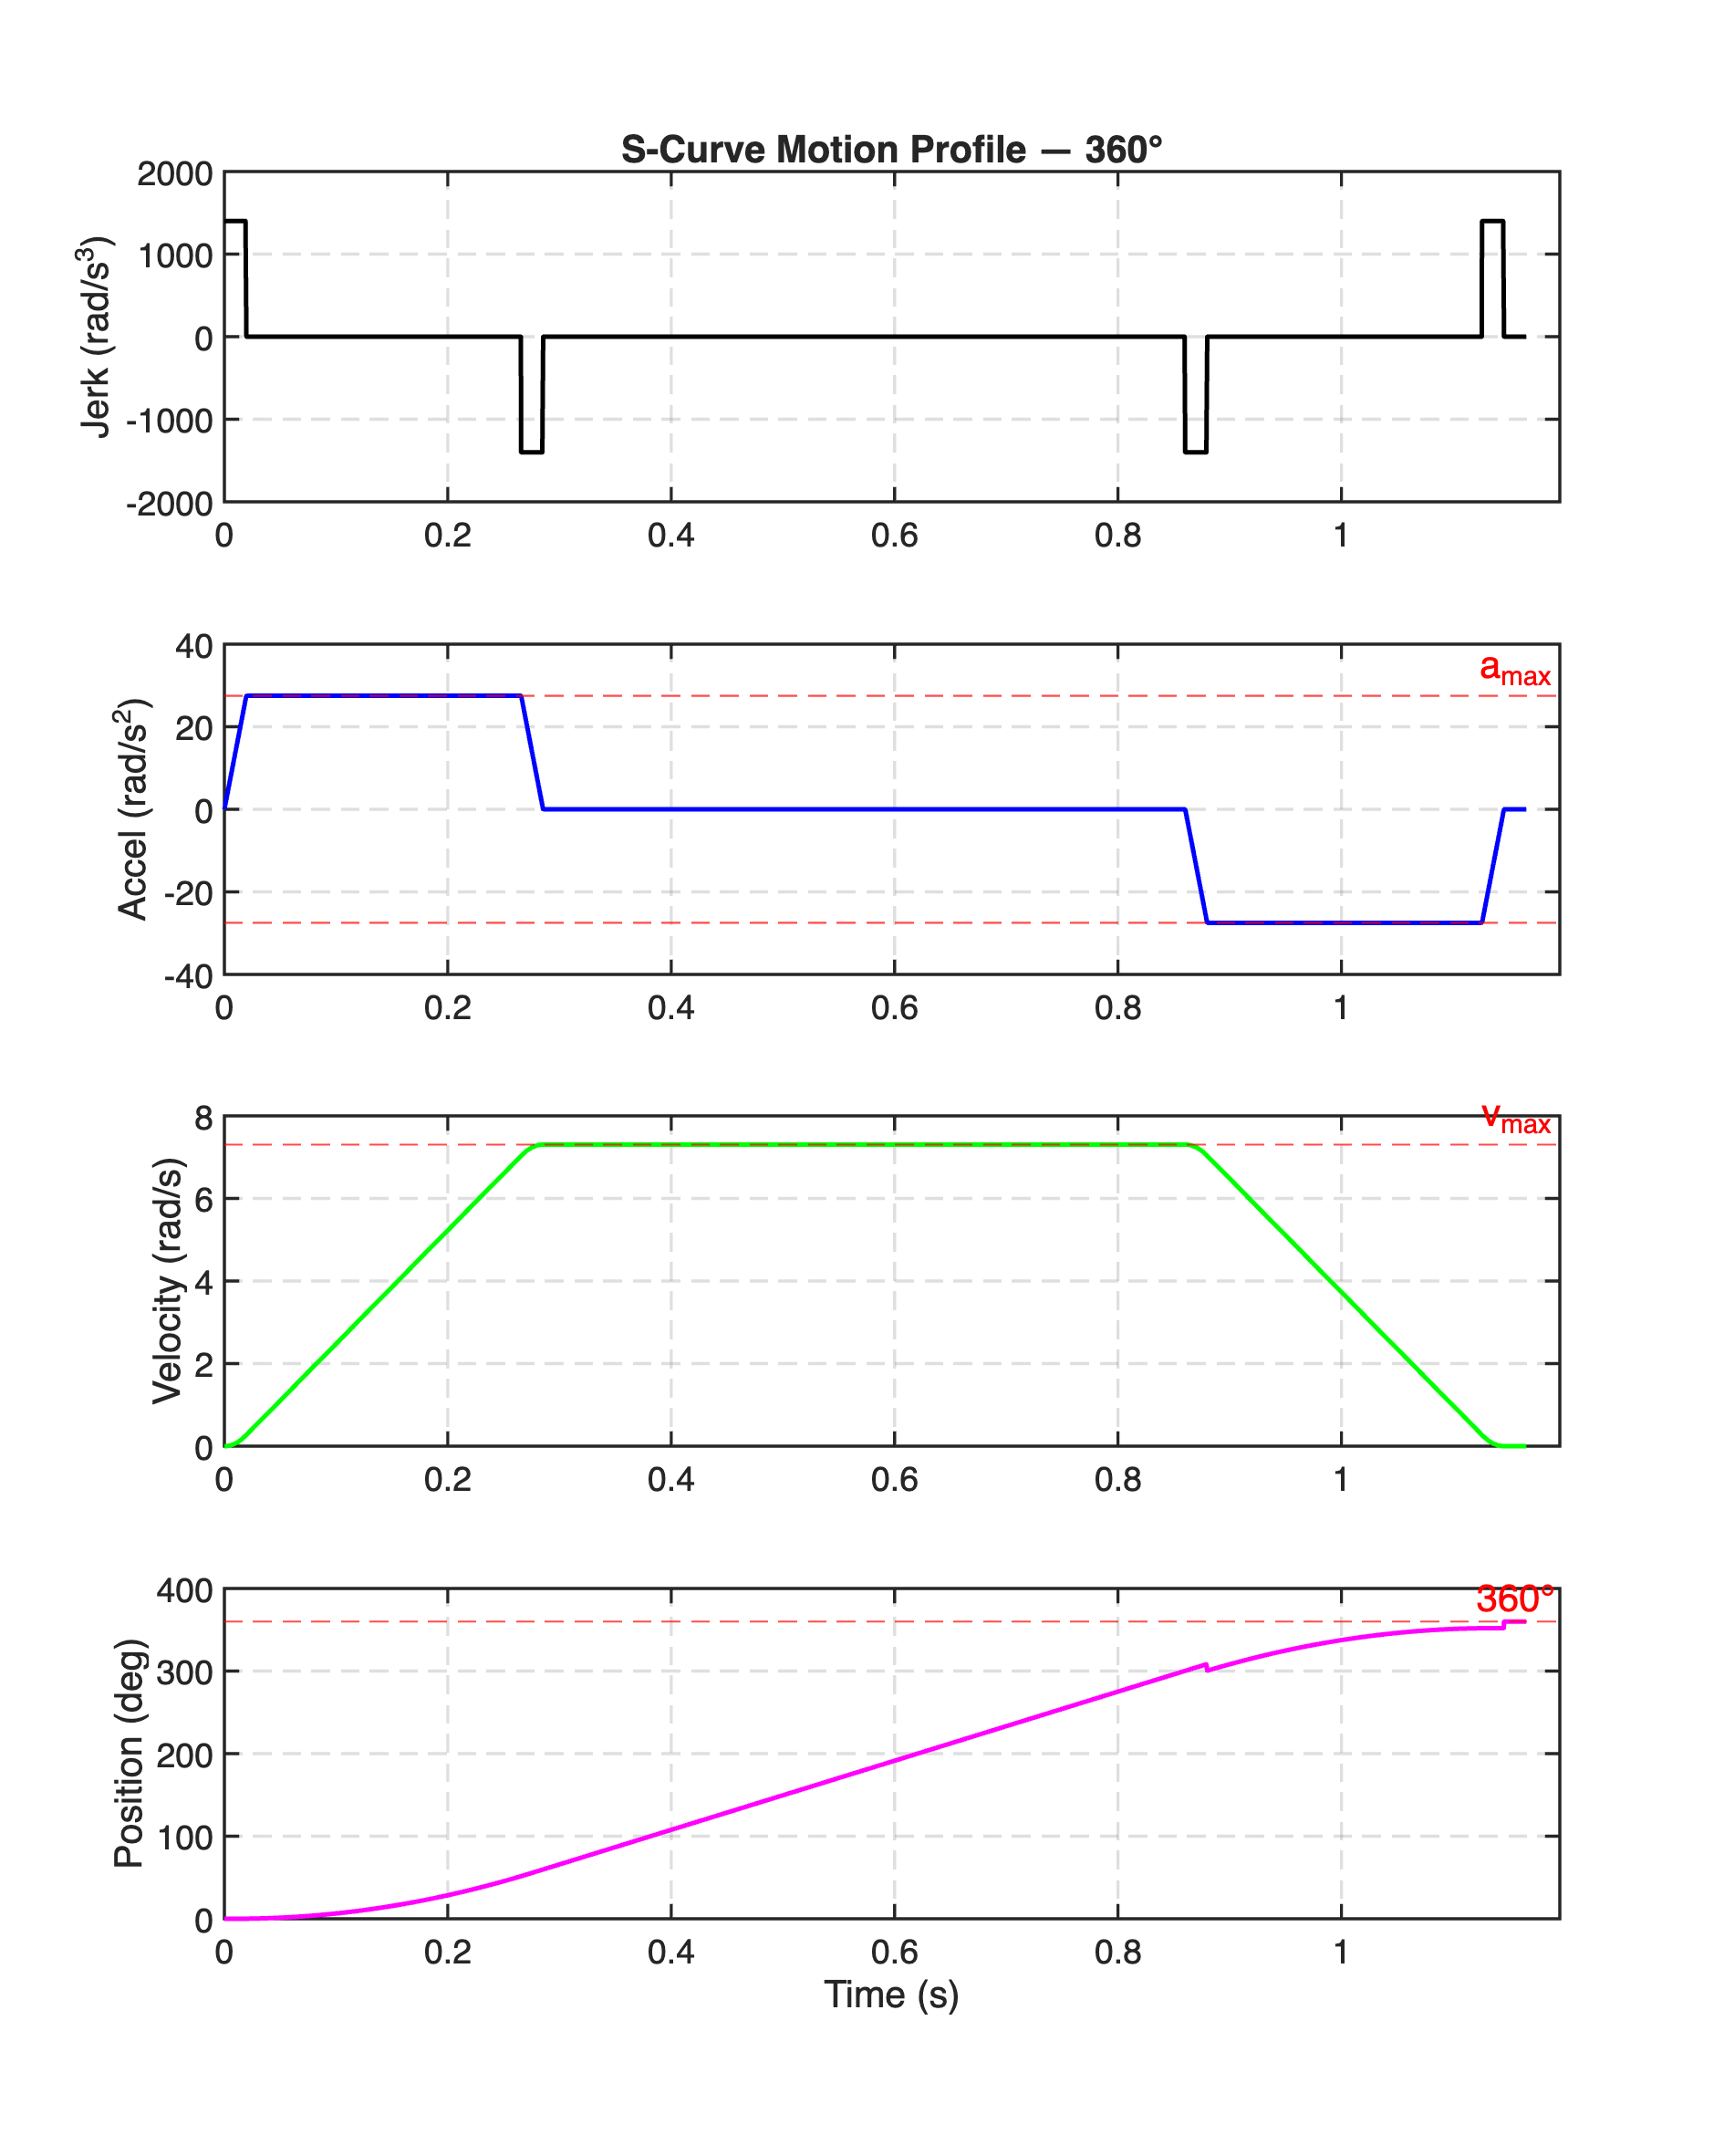
\includegraphics[width=0.88\textwidth]{images/scurve_360.png}
  \caption{S-Curve Motion Profile สำหรับการเคลื่อนที่ 360°
           แสดง Jerk, Acceleration, Velocity และ Position เทียบกับเวลา}
  \label{fig:scurve_360}
\end{figure}

\begin{table}[H]
  \centering
  \caption{สรุปพารามิเตอร์ Motion Profile สำหรับระยะทางต่าง ๆ}
  \label{tab:motion_summary}
  \begin{tabular}{lcccc}
    \toprule
    ระยะทาง & $q_{total}$ (rad) & $t_v$ (s) & $t_{move}$ (s) & หมายเหตุ \\
    \midrule
    90°  & $\pi/2 = 1.571$ & 0 (ไม่มี Cruise) & 0.571 & Triangle profile \\
    180° & $\pi = 3.142$   & 0.197            & 0.748 & -- \\
    360° & $2\pi = 6.283$  & 0.575            & 1.146 & Worst Case \\
    \bottomrule
  \end{tabular}
\end{table}

% ------------------------------------------------------------
\subsubsection{การ Simulation ด้วย State Space Model}
% ------------------------------------------------------------

\paragraph{State Space Model}

สร้างแบบจำลอง State Space 3 State สำหรับ Simulation
โดยเลือก State Vector $\mathbf{x} = \begin{bmatrix} i_a & \omega_{arm} & \theta_{arm} \end{bmatrix}^T$

\begin{equation}
  \dot{\mathbf{x}} = A\mathbf{x} + Bu_{in}, \qquad \mathbf{y} = C\mathbf{x}
  \label{eq:ss}
\end{equation}

\begin{equation}
  A = \begin{bmatrix}
        -R_a/L_a       & -K_b N/L_a & 0 \\
        K_t\eta N/J    & -b/J       & 0 \\
        0              & 1          & 0
      \end{bmatrix}
    = \begin{bmatrix}
        -1003.5 & -2013.0 & 0 \\
        3.265   & -0.265  & 0 \\
        0       & 1       & 0
      \end{bmatrix}
  \label{eq:A_matrix}
\end{equation}

\begin{equation}
  B = \begin{bmatrix} 1/L_a \\ 0 \\ 0 \end{bmatrix}
    = \begin{bmatrix} 690.6 \\ 0 \\ 0 \end{bmatrix}, \qquad
  C = \begin{bmatrix} 0 & 1 & 0 \\ 0 & 0 & 1 \end{bmatrix}
  \label{eq:BC_matrix}
\end{equation}

Discrete ด้วยวิธี Zero-Order Hold (ZOH) ที่ Sampling Period $T_s = 0.1$\,ms
ซึ่งน้อยกว่า Electrical Time Constant $\tau_{elec} = L_a/R_a = 1.0$\,ms อย่างน้อย 10 เท่า

\paragraph{ผลการ Simulation}

การประเมินสมรรถนะของ Cascade PID Control พร้อม S-Curve 360° กระทำผ่าน State Space Simulation เพื่อตรวจสอบการตอบสนองเชิงเวลา (Time Response) และพฤติกรรมของกระแสมอเตอร์ โดยผลการ Simulation โดยละเอียดแสดงใน\cref{subsec:sim_results_arm}

\subsection{การวิเคราะห์ผลกระทบของ Connection Rod ต่อ Cycle Time}

\subsubsection{ที่มาของปัญหา}

ในการใช้งานจริง Connection Rod จะแกว่งเมื่อแขนกลเร่งและหยุด ซึ่งอาจทำให้ไม่สามารถสวม Rod เข้ารูขนาด 14 mm ได้หากมุมแกว่งยังสูงอยู่

\subsubsection{แบบจำลอง Connection Rod}

Connection Rod มีมวล $m_{rod} = 164.08$\,g และความยาว $L_{rod} = 100$\,mm จำลองเป็น Simple Pendulum ที่ถูกกระตุ้นด้วย Angular Acceleration ของแขนกล

สมการการเคลื่อนที่ของ Rod (Linearized) คือ

\begin{equation}
  I_{pivot}\,\ddot{\phi} = -m_{rod}\,g\,l_{cm}\,\phi
                          - 2\zeta_{rod}\,\omega_{n,rod}\,I_{pivot}\,\dot{\phi}
                          - m_{rod}\,l_{cm}\,r_{arm}\,\alpha_{arm}
  \label{eq:rod_eom}
\end{equation}

ค่า Natural Frequency และ Damping Ratio ของ Rod คือ

\begin{equation}
  \omega_{n,rod} = \sqrt{\frac{m_{rod}\,g\,l_{cm}}{I_{pivot}}}
                = 12.13\,\text{rad/s}
                \quad (\,f_n = 1.93\,\text{Hz})
  \label{eq:wn_rod}
\end{equation}

\begin{equation}
  \zeta_{rod} = 0.05 \quad \Rightarrow \quad
  t_{settle,rod} \approx \frac{3}{\zeta_{rod}\,\omega_{n,rod}} \approx 4.95\,\text{s}
  \label{eq:rod_settle}
\end{equation}

\subsubsection{ข้อจำกัดด้านความแม่นยำในการ Pick และ Place}

Clearance เพียง 1\,mm ต่อข้าง ทำให้มุมแกว่งสูงสุดที่ยอมรับได้คือ

\begin{equation}
  \phi_{max} = \arcsin\!\left(\frac{1\,\text{mm}}{100\,\text{mm}}\right) \approx 0.57°
  \label{eq:phi_max}
\end{equation}

\subsubsection{การวิเคราะห์ Input Shaping และ Multi-objective Optimization}

จากการวิเคราะห์พบว่าการใช้ S-Curve Profile เพียงอย่างเดียวไม่เพียงพอในการลดการแกว่งของ Rod จึงจำเป็นต้องใช้เทคนิค Input Shaping และ NSGA-II ในการปรับพารามิเตอร์ของระบบ

\begin{equation}
  \begin{split}
    t_2 &= \frac{\pi}{\omega_{d,rod}} = \frac{\pi}{12.115} = 0.2593\,\text{s} \\
    A_1 &= \frac{1}{1+K_{ZV}} = 0.5392, \qquad
    A_2  = \frac{K_{ZV}}{1+K_{ZV}} = 0.4608
  \end{split}
  \label{eq:zv_params}
\end{equation}

การดำเนินการค้นหาค่าพารามิเตอร์ที่เหมาะสมที่สุด (Optimization) กระทำผ่านอัลกอริทึม NSGA-II เพื่อหาจุดสมดุลระหว่าง Cycle Time และ Rod Swing โดยผลการวิเคราะห์ Pareto Front และ Solution ที่เลือกแสดงใน\cref{subsec:rod_opt_results}

\subsubsection{สรุปผลและข้อจำกัดที่พบ}

ผลการวิเคราะห์แสดงให้เห็นข้อจำกัดทางกายภาพของการแก้ปัญหาด้วย Software เพียงอย่างเดียว ซึ่งนำไปสู่ข้อเสนอแนะในการปรับปรุงระบบในขั้นตอนถัดไป โดยรายละเอียดการวิเคราะห์แสดงใน\cref{subsec:rod_opt_results}

% ============================================================================
% FILE: sections/03_implementation.tex
% PURPOSE: การติดตั้งจริง Mechanical / Electronics / STM32 Firmware
% ============================================================================

\section{การดำเนินการสร้างและติดตั้งระบบ (Implementation)}

% ============================================================
\subsection{การประกอบเชิงกล (Mechanical Assembly)}
% ============================================================

\subsubsection{ลำดับขั้นตอนการประกอบ}
% อธิบายลำดับการประกอบจากฐานถึง End Effector

\subsubsection{ผลการประกอบชิ้นส่วน}

% \begin{figure}[H]
%   \centering
%   \includegraphics[width=0.75\textwidth]{images/assembly_photo.jpg}
%   % [ใส่ภาพถ่ายจริงของ Assembly ที่ประกอบเสร็จ --- ด้านหน้า/ด้านข้าง]
%   \caption{หุ่นยนต์หลังการประกอบเสร็จสมบูรณ์}
%   \label{fig:assembly_photo}
% \end{figure}

\subsubsection{การตรวจสอบขนาดจริง}
% ผลการวัดขนาดฐานจริง เทียบกับ M1 (<= 200x200 mm)

\begin{table}[H]
  \centering
  \caption{ผลการตรวจสอบขนาดชิ้นส่วนจริง}
  \label{tab:mech_dim_check}
  % [ตาราง: รายการ | ค่าออกแบบ | ค่าวัดจริง | Req ID | Pass/Fail]
\end{table}

% ============================================================
\subsection{การประกอบตู้ควบคุมไฟฟ้า (Electrical Cabinet Assembly)}
% ============================================================

\subsubsection{รายการอุปกรณ์ภายในตู้}

\begin{table}[H]
  \centering
  \caption{Bill of Materials (BOM) ของตู้ควบคุม}
  \label{tab:elec_bom}
  % [ตาราง: อุปกรณ์ | รุ่น | จำนวน | หน้าที่]
\end{table}

\subsubsection{ผลการประกอบตู้ควบคุม}
% สถานะ: กำลังดำเนินการ --- จะอัปเดตหลังประกอบเสร็จ

% \begin{figure}[H]
%   \centering
%   \includegraphics[width=0.70\textwidth]{images/cabinet_interior.jpg}
%   % [ใส่ภาพถ่ายภายในตู้ควบคุมหลังประกอบเสร็จ]
%   \caption{ภายในตู้ควบคุมหลังการประกอบ}
%   \label{fig:cabinet_interior}
% \end{figure}

% \begin{figure}[H]
%   \centering
%   \includegraphics[width=0.70\textwidth]{images/cabinet_front.jpg}
%   % [ใส่ภาพถ่ายหน้าตู้ แสดง Power Indicator, E-Stop, Mode Switch]
%   \caption{หน้าตู้ควบคุมแสดงสวิตช์และไฟแสดงสถานะ}
%   \label{fig:cabinet_front}
% \end{figure}

% ============================================================
\subsection{สถาปัตยกรรม STM32 Firmware (Firmware Architecture)}
% ============================================================

\subsubsection{ภาพรวมสถาปัตยกรรม Firmware}
% อธิบายว่า Firmware ทำงานอย่างไรโดยรวม
% ระบุ Main Loop, Interrupt, Task ต่างๆ

% \begin{figure}[H]
%   \centering
%   \includegraphics[width=0.85\textwidth]{images/firmware_arch_block.png}
%   % [ใส่ Block Diagram ของ Firmware: Main Loop, ISR, Module ต่างๆ]
%   \caption{ภาพรวมสถาปัตยกรรม STM32 Firmware}
%   \label{fig:fw_arch}
% \end{figure}

\subsubsection{โครงสร้างไฟล์และโมดูล (Code Structure)}
% Folder Structure และหน้าที่ของแต่ละ Module

\begin{table}[H]
  \centering
  \caption{โมดูลหลักใน STM32 Firmware}
  \label{tab:fw_modules}
  % [ตาราง: ชื่อไฟล์ | หน้าที่ | Peripheral ที่ใช้ | สถานะ]
\end{table}

\subsubsection{Interrupt Service Routine (ISR) และ Timing}
% ISR ที่ใช้ เช่น Encoder ISR, Timer ISR สำหรับ PID Loop

\begin{table}[H]
  \centering
  \caption{ISR และ Task Timing ของ Firmware}
  \label{tab:fw_timing}
  % [ตาราง: ISR/Task | Trigger | Period/Priority | หน้าที่]
\end{table}

\subsubsection{การทำงานร่วมกันของโมดูล (Module Interaction)}
% Encoder -> PID -> PWM Output

% \begin{figure}[H]
%   \centering
%   \includegraphics[width=0.85\textwidth]{images/firmware_dataflow.png}
%   % [ใส่ Data Flow Diagram ระหว่าง Module ต่างๆ ใน Firmware]
%   \caption{Data Flow ระหว่างโมดูลใน Firmware}
%   \label{fig:fw_dataflow}
% \end{figure}

\subsubsection{การ Implement S-Curve Motion Profile ใน Firmware}
% วิธีการแปลง S-Curve ที่คำนวณได้มาเป็น Code จริงบน STM32
% อธิบาย State Machine ของ Motion Profile

\subsubsection{Joystick Mode และการ Map ปุ่ม}
% โหมดที่ใช้งานได้ทั้งหมด: Manual, Auto, Homing
% อ้างอิง J1, E8

\begin{table}[H]
  \centering
  \caption{การ Map ปุ่ม Joystick กับคำสั่งระบบ}
  \label{tab:joystick_map}
  % [ตาราง: ปุ่ม | โหมด | คำสั่งที่ส่ง | Req ID]
\end{table}
% ============================================================
\section{การบูรณาการระบบ (System Integration)}
\label{sec:system_integration}
% ============================================================

\subsection{สถาปัตยกรรมการบูรณาการ}
\label{subsec:integration_architecture}

การบูรณาการระบบเชื่อมต่อ Subsystem ทั้งหมด 4 ส่วน
ได้แก่ Mechanical, Electrical, Firmware และ
External Application เข้าด้วยกันผ่าน Interface
ที่กำหนดไว้ใน System Architecture

% [รูปที่ XX: Integration Diagram ของระบบทั้งหมด]
% \begin{figure}[H]
%   \centering
%   \includegraphics[width=0.95\textwidth]{images/integration_diagram.png}
%   \caption{Integration Diagram ของระบบทั้งหมด}
%   \label{fig:integration_diagram}
% \end{figure}

% ------------------------------------------------------------
\subsection{การเชื่อมต่อ STM32 กับ Motor และ Encoder}
\label{subsec:stm32_motor_encoder_connection}
% ------------------------------------------------------------

STM32G474RE เชื่อมต่อกับ Motor และ Encoder
ผ่าน Peripheral ดังนี้

\begin{itemize}
  \item \textbf{Encoder}: AMT-103 ต่อกับ TIM3
        ในโหมด \texttt{TIM\_ENCODERMODE\_TI12}
        (4x Quadrature) ผ่าน Pin PB4 (CH A)
        และ PB5 (CH B) Counter Range 0--65535
        Resolution = $2048 \times 4 \times 70
        = 573{,}440$ counts/rev ที่ Output shaft

  \item \textbf{PWM}: TIM8 CH2 บน Pin PA8
        Prescaler = 169, Period = 50
        ได้ $f_{PWM} = 170\,\text{MHz}
        / (170 \times 51) \approx 19.6\,\text{kHz}$
        ทิศทางควบคุมผ่าน GPIO PC6 (DIR)

  \item \textbf{Motor Driver}: Cytron MD10C
        รับ PWM และ DIR จาก STM32 โดยตรง
        ผ่าน Optocoupler Module เพื่อแยก Ground
\end{itemize}

ผลการทดสอบการอ่านค่า Encoder และสัญญาณ PWM
แสดงดังรูปที่~\ref{fig:encoder_pwm_test}

% [รูปที่ XX: ผลการทดสอบการอ่านค่า Encoder และสัญญาณ PWM]
% \begin{figure}[H]
%   \centering
%   \includegraphics[width=0.88\textwidth]{images/encoder_pwm_test.png}
%   \caption{ผลการทดสอบการอ่านค่า Encoder และสัญญาณ PWM
%            แสดง Count และมุมที่คำนวณได้แบบ Real-time}
%   \label{fig:encoder_pwm_test}
% \end{figure}

% ------------------------------------------------------------
\subsection{การเชื่อมต่อ Joystick}
\label{subsec:joystick_connection}
% ------------------------------------------------------------

Joystick เชื่อมต่อกับ STM32 ผ่าน ESP32-DEVKIT-V1
ซึ่งทำหน้าที่เป็น Bluetooth Receiver
รับสัญญาณจาก Wireless Joystick แล้วแปลงเป็น
Command Character ส่งต่อผ่าน USART3
ที่ Baud Rate 115200\,bps, 8N1

การทดสอบครอบคลุมทุกโหมดการทำงาน
ได้แก่ Manual Mode และ Auto Mode
โดย E-Stop ทำงานได้ทุกโหมดตามข้อกำหนด J1

\begin{table}[H]
  \centering
  \caption{ผลการทดสอบ Joystick แต่ละโหมด}
  \label{tab:joystick_test}
  \begin{tabular}{lllc}
    \toprule
    โหมด & ปุ่มที่ทดสอบ & พฤติกรรมที่สังเกตได้ & ผล \\
    \midrule
    Manual
      & หมุนซ้าย (\texttt{L})
      & แขนหมุนซ้ายตาม Step ที่กำหนด
      & ผ่าน \\
    Manual
      & หมุนขวา (\texttt{R})
      & แขนหมุนขวาตาม Step ที่กำหนด
      & ผ่าน \\
    Manual
      & Gripper Pick (\texttt{S})
      & Gripper ทำ Sequence Pick ครบ
      & ผ่าน \\
    Manual
      & Gripper Place (\texttt{G})
      & Gripper ทำ Sequence Place ครบ
      & ผ่าน \\
    ทุกโหมด
      & Home (\texttt{A} Hold)
      & แขนเคลื่อนกลับตำแหน่ง 0°
      & ผ่าน \\
    ทุกโหมด
      & E-Stop (\texttt{P})
      & มอเตอร์หยุดทันที PWM = 0
      & ผ่าน \\
    ทุกโหมด
      & Reset E-Stop (\texttt{P} ซ้ำ)
      & ระบบกลับสู่ Ready State
      & ผ่าน \\
    Manual
      & สลับ Coarse/Fine (\texttt{M})
      & Jog Mode สลับระหว่าง Step/Jog
      & ผ่าน \\
    \bottomrule
  \end{tabular}
\end{table}

% ------------------------------------------------------------
\subsection{การเชื่อมต่อ Modbus กับ Base System}
\label{subsec:modbus_connection}
% ------------------------------------------------------------

STM32G474RE ทำงานเป็น Modbus RTU Slave
บน LPUART1 ที่ Slave Address 21,
Baud Rate 19200\,bps, 8E1
รองรับ Function Code 0x03 (Read Holding Registers)
และ 0x06 (Write Single Register)
ทดสอบการสื่อสารด้วย QModMaster

\paragraph{Modbus Register Map}

\begin{table}[H]
  \centering
  \caption{Modbus Register Map (Slave Address 21)}
  \label{tab:modbus_map}
  \begin{tabular}{lllp{5.5cm}}
    \toprule
    Address (Hex) & ประเภท & ชื่อ & คำอธิบาย \\
    \midrule
    \multicolumn{4}{l}{\textit{Write Registers (Master $\rightarrow$ Slave)}} \\
    \midrule
    0x00 & R    & Device ID    & ค่าคงที่ 22881 (``YA'') Heartbeat \\
    0x01 & R/W  & Command Bits &
      Bit0: Go Home,
      Bit1: Jog/Gripper Manual,
      Bit2: Auto Mode,
      Bit3: Set Home (Reset Encoder),
      Bit4: Test Mode \\
    0x02 & R/W  & Gripper Cmd  &
      0=Up, 1=Down, 2=Open, 4=Close
      (ใช้คู่กับ Bit1 ของ 0x01) \\
    0x03 & R/W  & Gripper Seq  & 1=Pick Sequence, 2=Place Sequence \\
    0x05 & R/W  & Jog Step     & ระยะ Jog (deg, signed int16) \\
    0x24 & R/W  & Target Pos   & ตำแหน่งเป้าหมาย (deg, signed int16) \\
    0x25 & R/W  & Safety Bits  & Bit0: E-Stop, Bit1: Reset E-Stop \\
    \midrule
    \multicolumn{4}{l}{\textit{Read Registers (Slave $\rightarrow$ Master)}} \\
    \midrule
    0x26 & R    & Reed Sensors & สถานะ Reed Switch (ปัจจุบัน = 0) \\
    0x27 & R    & Task Status  &
      Bit1: Position Mode Active,
      Bit2: Ghost Move Active \\
    0x28 & R    & Current Pos  & ตำแหน่งปัจจุบัน ($\times$10, signed int16) \\
    0x29 & R    & Current Speed& ความเร็วปัจจุบัน ($\times$10, signed int16) \\
    0x30 & R    & Acceleration & ความเร่งปัจจุบัน (ปัจจุบัน = 0) \\
    0x31 & R    & Safety Status& 0=Normal, 1=E-Stop Active \\
    \bottomrule
  \end{tabular}
\end{table}

หมายเหตุ: ค่าตำแหน่งที่ Register 0x28 สเกล $\times 10$
เพื่อให้ส่งค่า Decimal ได้ผ่าน Integer Register
เช่น ตำแหน่ง 90.5° ส่งเป็น 905

% ------------------------------------------------------------
\subsection{แผนการทดสอบ End-to-End}
\label{subsec:end_to_end_test_plan}
% ------------------------------------------------------------

\begin{table}[H]
  \centering
  \caption{แผนการทดสอบ End-to-End}
  \label{tab:e2e_plan}
  \begin{tabular}{clp{4.5cm}lc}
    \toprule
    \# & Test Case & เกณฑ์วัดผลสำเร็จ & Requirements & สถานะ \\
    \midrule
    1 & Encoder + PWM Verification
      & อ่านค่ามุมได้ถูกต้อง $\pm$[THRESH]°,
        PWM ควบคุมความเร็วได้
      & M4, A2
      & ผ่าน \\
    2 & E-Stop Hardware Interlock
      & กด E-Stop มอเตอร์หยุดทันที,
        STM32 ยังมีไฟ
      & E6, E7
      & ผ่าน \\
    3 & Joystick Manual Control
      & ควบคุมทุกปุ่มได้ถูกต้อง
        Response Time $<$100\,ms
      & E8, J1
      & ผ่าน \\
    4 & Modbus Read/Write
      & QModMaster อ่าน 0x28 ได้ค่าตำแหน่งจริง,
        เขียน 0x24 แล้วแขนเคลื่อนที่
      & E1
      & ผ่าน \\
    5 & PID Closed-Loop (No Load)
      & Settling Time $\leq$0.5\,s,
        Overshoot $\leq$1\%
      & P5, P6
      & รอ Tune \\
    6 & PID Closed-Loop (2\,kg Load)
      & Settling Time $\leq$0.5\,s,
        Overshoot $\leq$1\%
      & P5, P6, P7
      & รอ Tune \\
    7 & Full Auto Sequence (4 ชิ้น)
      & Cycle Time $\leq$35\,s
        ครบ 4 ชิ้นใน 1 รอบ
      & P1, P2
      & รอ Demo \\
    8 & Precision Test (100 รอบ)
      & Repeatability $\leq \pm$0.1°
      & A2
      & รอ Demo \\
    9 & Continuous Rotation 540°
      & สายไม่พันกัน ระบบทำงานปกติ
      & M9
      & รอ Demo \\
    \bottomrule
  \end{tabular}
\end{table}
% ============================================================================
% FILE: sections/05_test_results.tex
% PURPOSE: ผลการทดสอบ Unit Test และ System Test แยกตาม Progress
% ============================================================================

\section{ผลการทดสอบ (Test Results)}

% ============================================================
\subsection{ผลการทดสอบ Progress Update 1}
% ============================================================

\subsubsection{ผล FEA และการคำนวณ Deflection}
% อ้างอิง M3: $\delta_{\text{total}} = 0.237$ mm $< 1$ mm --- ผ่าน

\begin{table}[H]
  \centering
  \caption{ผล FEA เทียบกับเกณฑ์ M3}
  \label{tab:fea_p1}
  % [ตาราง: วิธี | delta (mm) | เกณฑ์ | ผล]
\end{table}

\subsubsection{ผลการคำนวณ Motion Profile (ทฤษฎี)}
% อ้างอิง P1: เวลารวม = 34.39 s < 35 s --- ผ่านในทฤษฎี

% ============================================================
\subsection{ผลการตรวจสอบความถูกต้องของแบบจำลอง (Model Validation)}
\label{subsec:model_validation_results}
% ============================================================

ในหัวข้อนี้แสดงผลการตรวจสอบความถูกต้องของแบบจำลอง (Transfer Function) ที่ได้จากการทำ System Identification โดยเปรียบเทียบระหว่างสัญญาณความเร็วเชิงมุมที่วัดได้จริงจาก Hardware ($y_{measured}$) กับสัญญาณที่ได้จากการ Simulate แบบจำลอง ($y_{simulated}$) ภายใต้สัญญาณ Excitation รูปแบบต่าง ๆ

\begin{figure}[H]
  \centering
  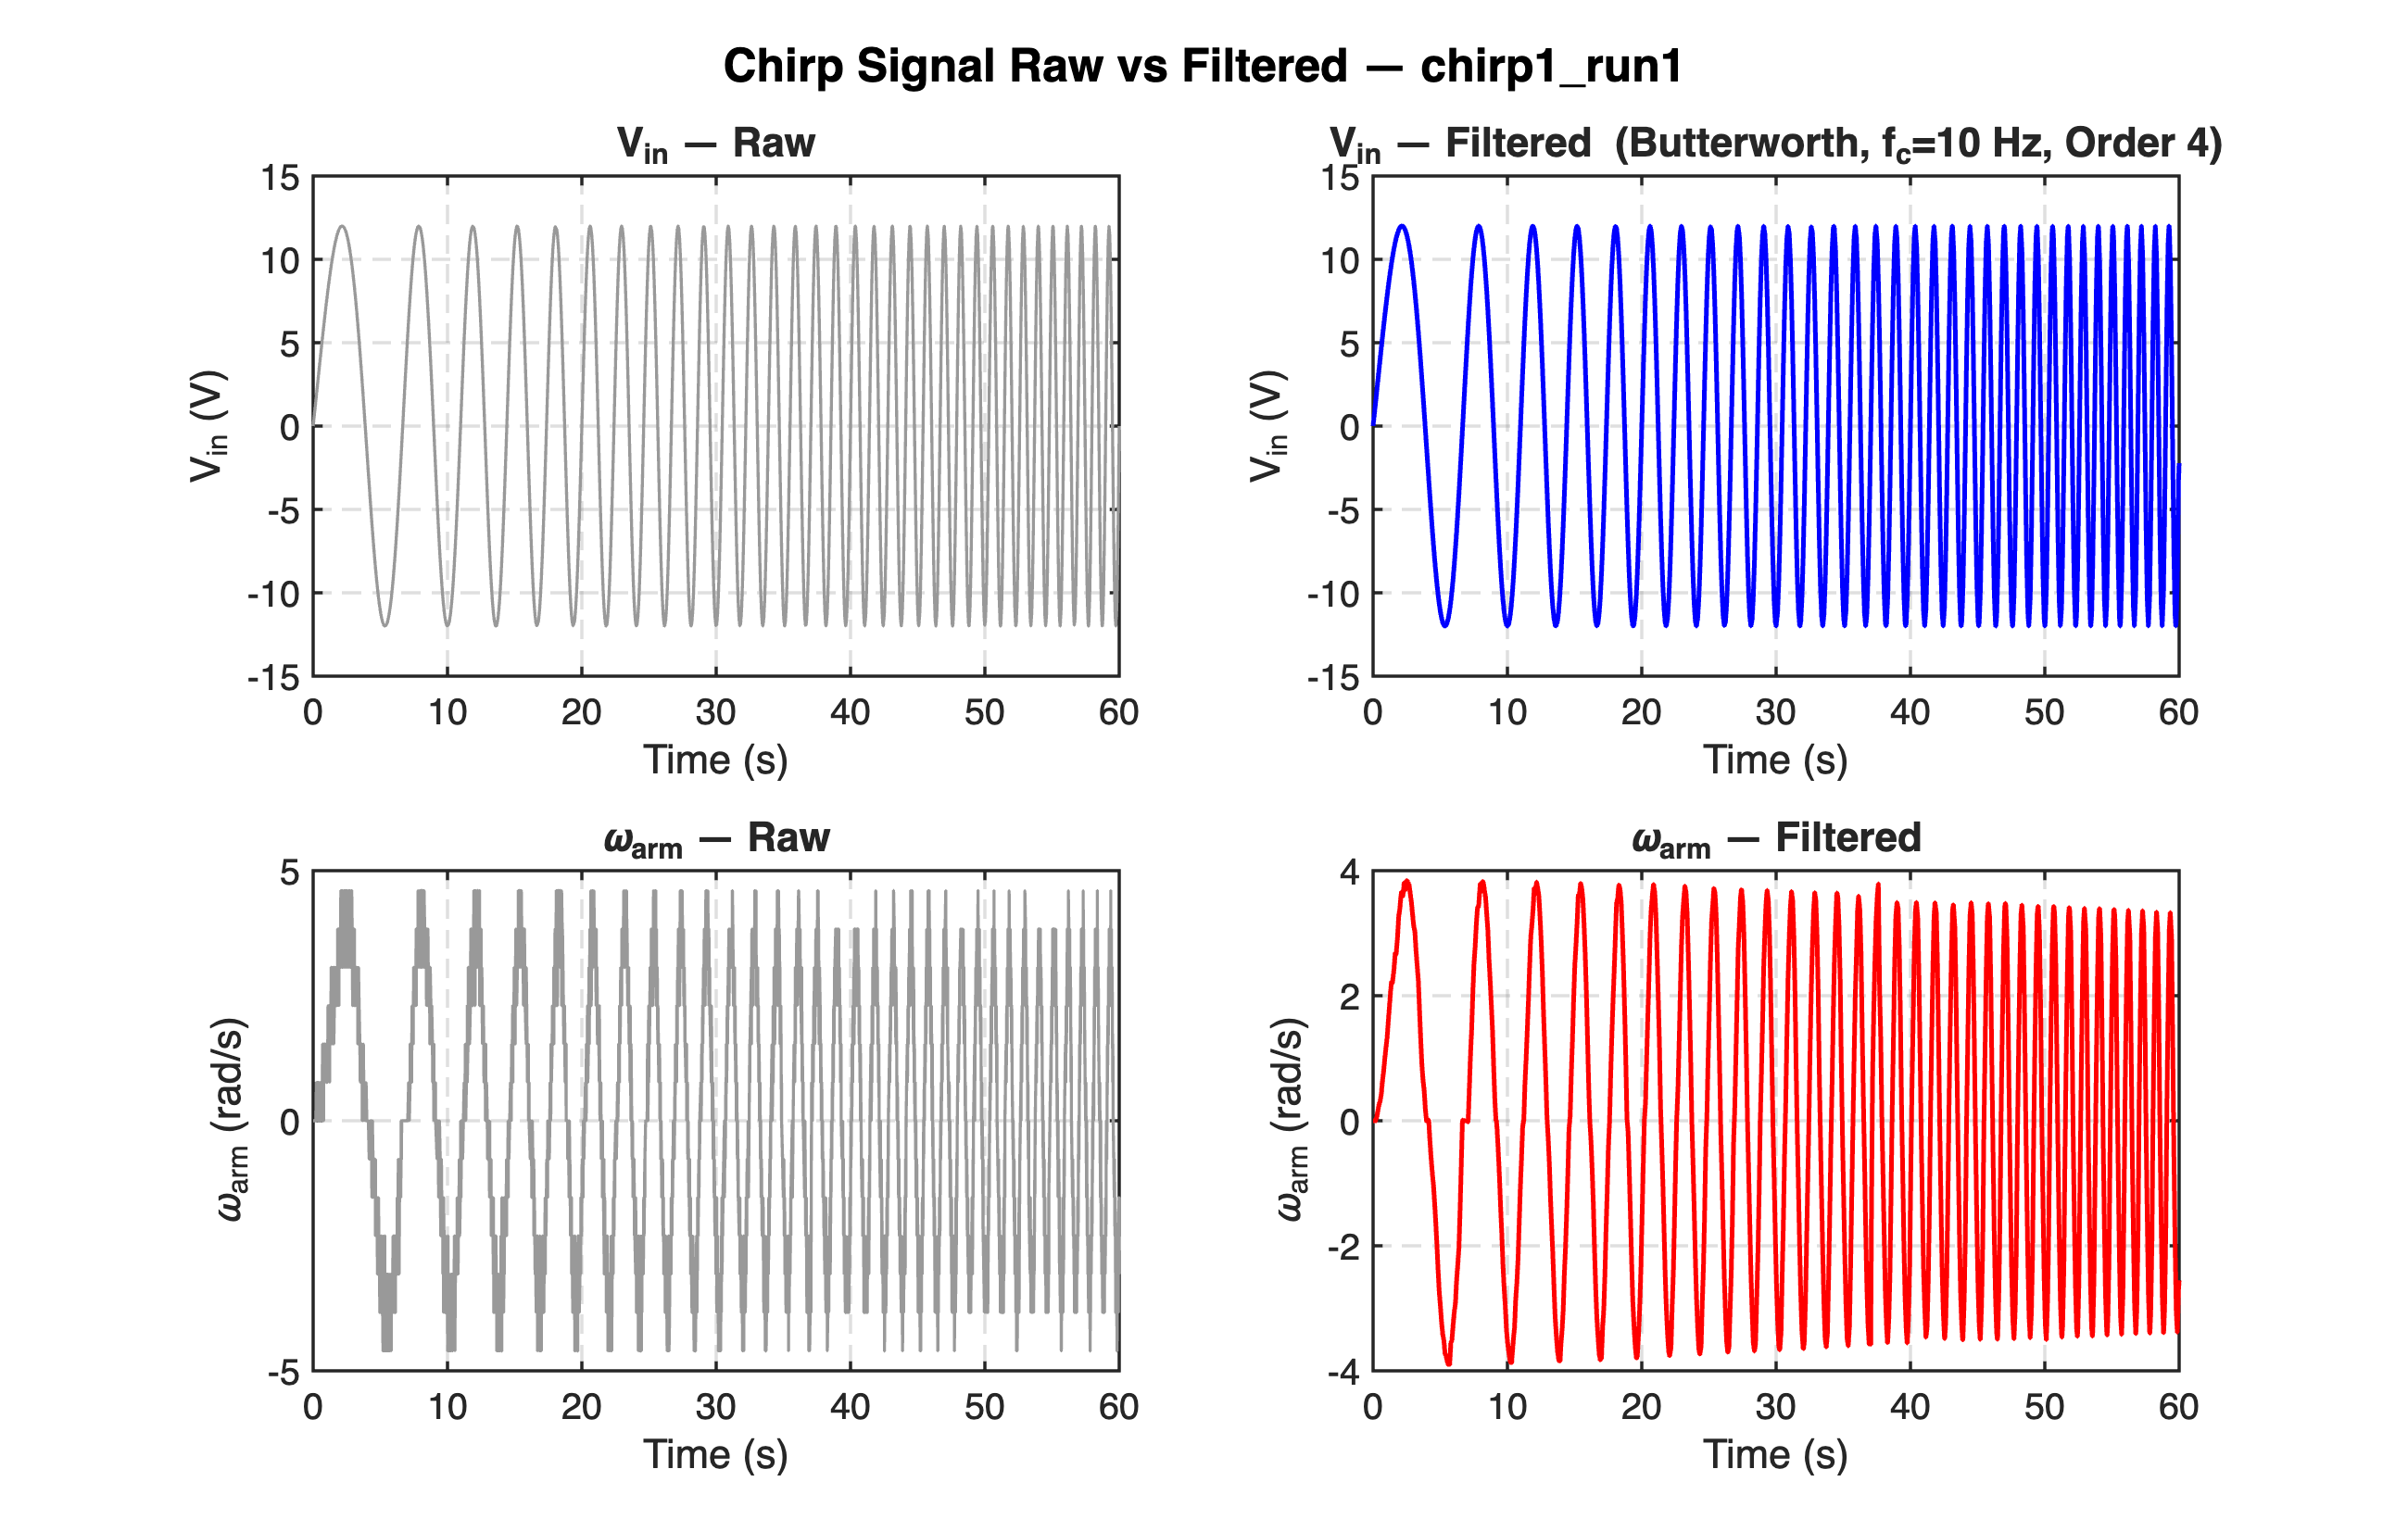
\includegraphics[width=0.88\textwidth]{images/chirp_raw_filtered.png}
  \caption{สัญญาณ Chirp ก่อนและหลัง Filter (chirp1\_run1) แสดง $V_{in}$ และ $\omega_{arm}$}
  \label{fig:chirp_filtered}
\end{figure}

\begin{figure}[H]
  \centering
  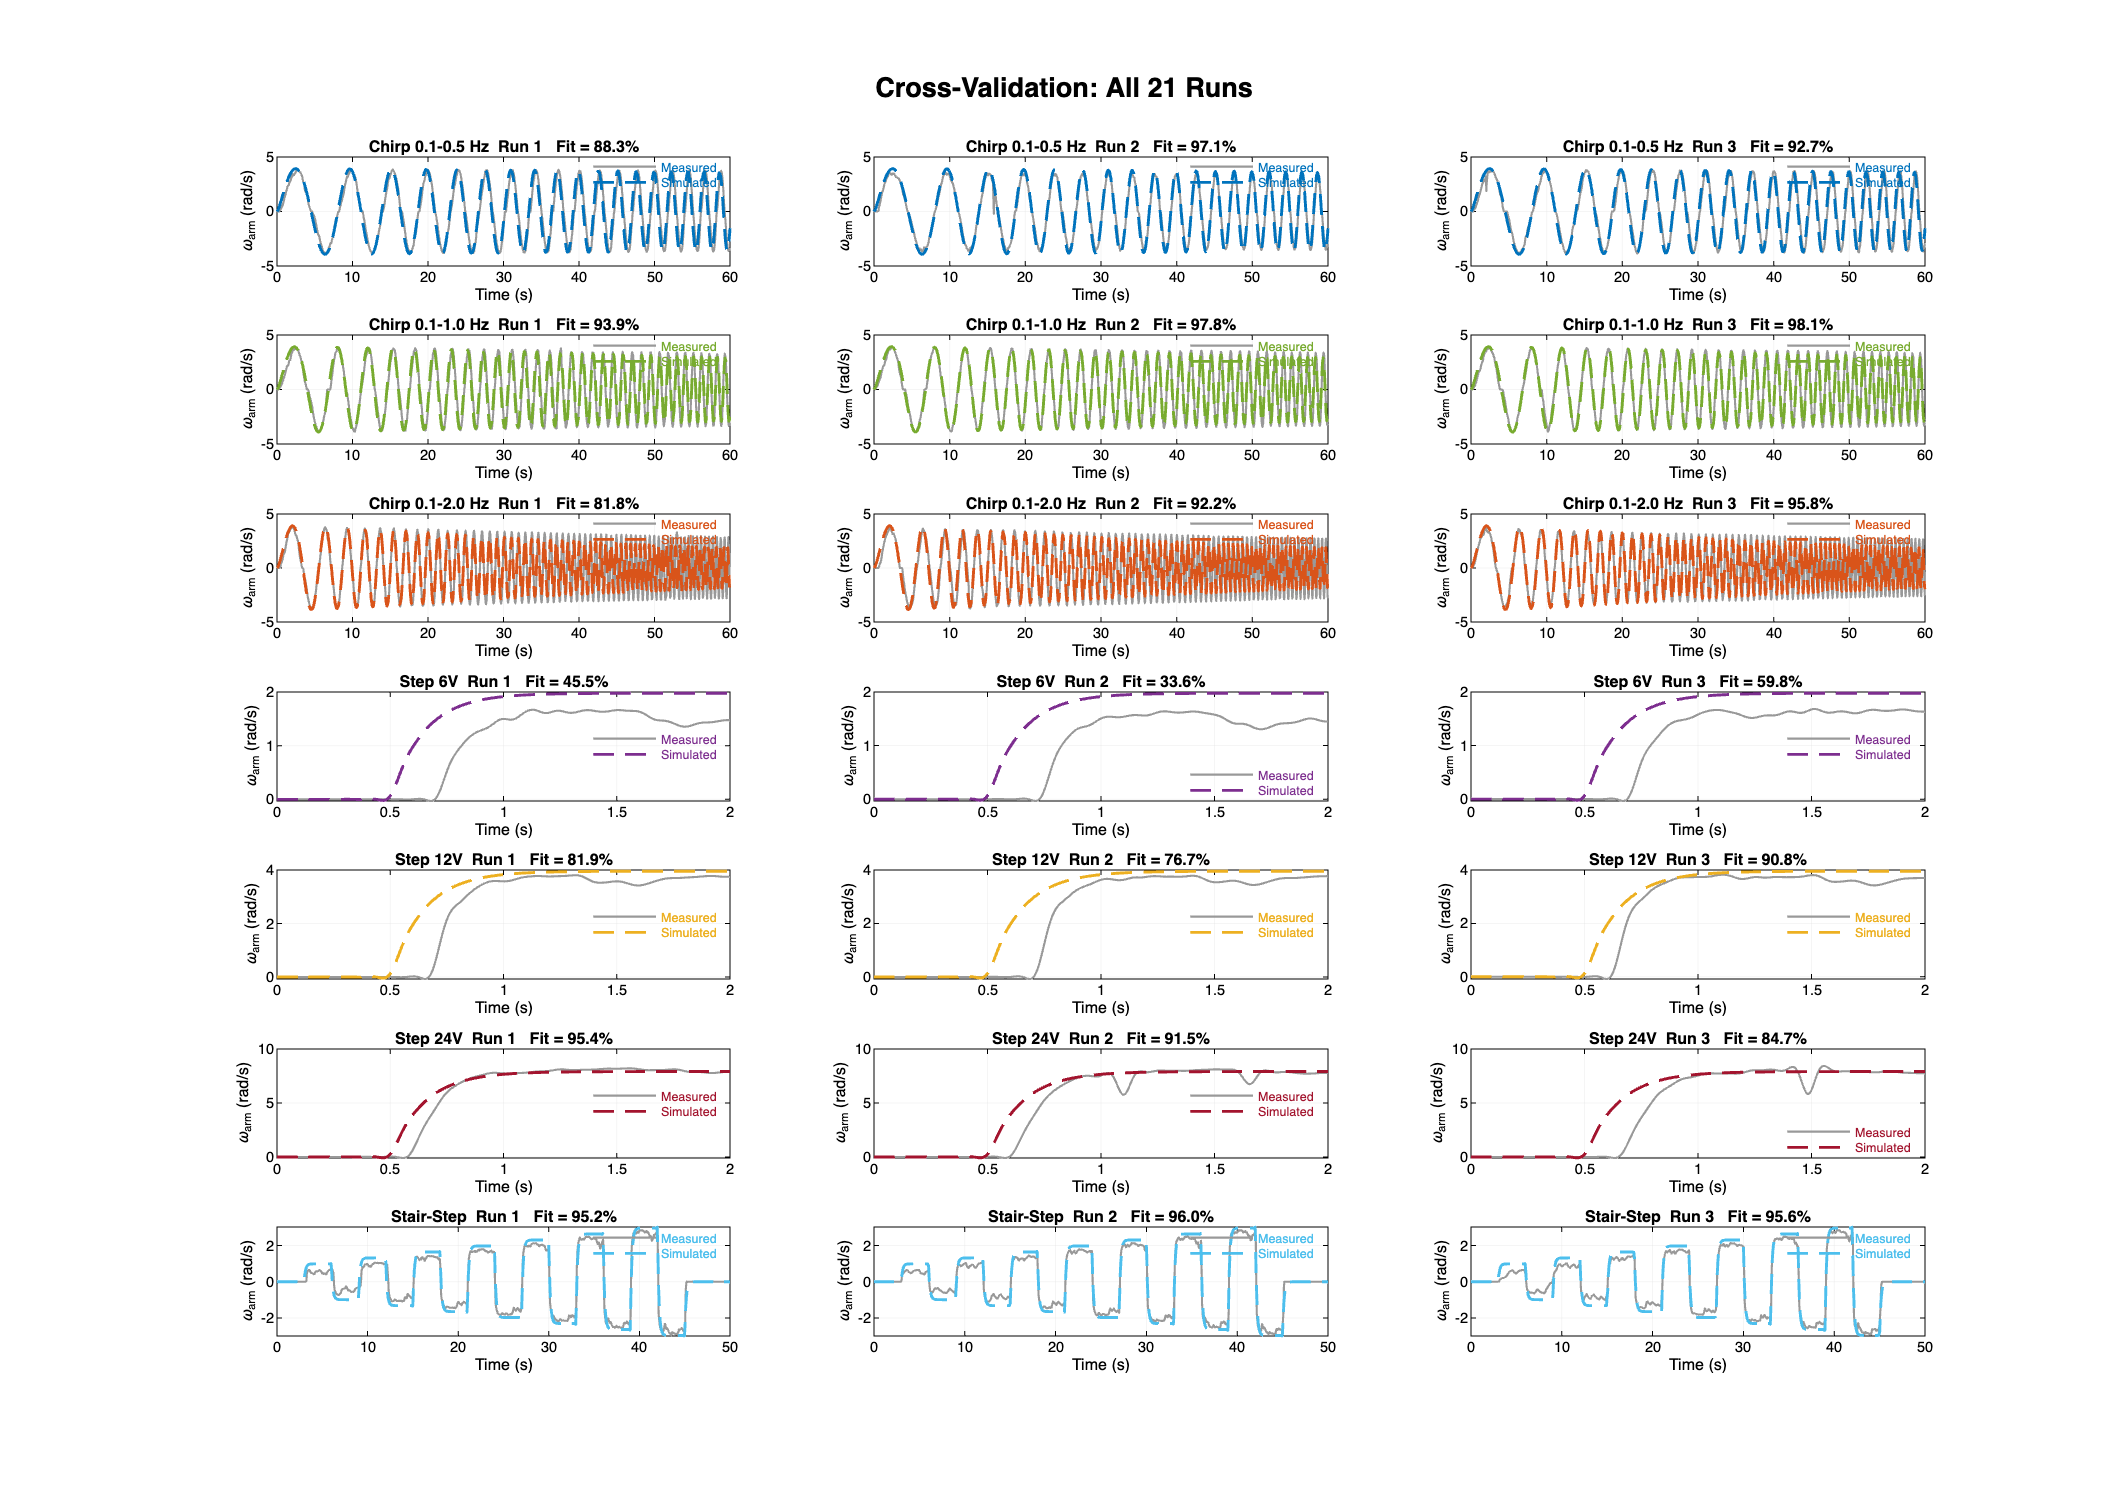
\includegraphics[width=1\textwidth]{images/cross_validation.png}
  \caption{เปรียบเทียบ Measured กับ Simulated สำหรับ Stair-Step data (3 runs)}
  \label{fig:cross_val}
\end{figure}

\begin{figure}[H]
  \centering
  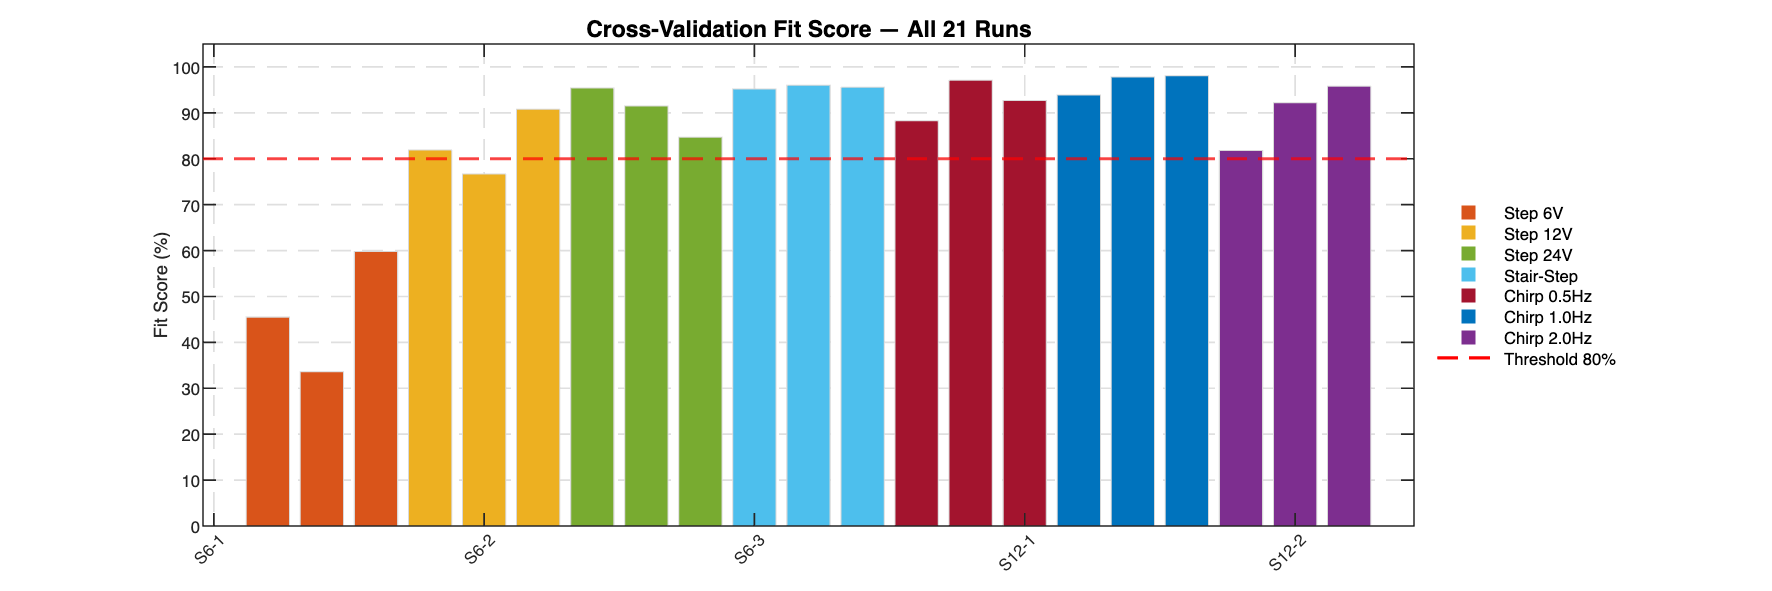
\includegraphics[width=0.88\textwidth]{images/cross_val_bar.png}
  \caption{Fit Score จาก Cross-Validation กับข้อมูลประเภทต่าง ๆ ทั้ง 21 runs
           (เส้นประแดงคือเกณฑ์ 80\%)}
  \label{fig:cross_val_bar}
\end{figure}

\begin{table}[H]
  \centering
  \caption{ผลการ Cross-Validation ของ Model กับข้อมูลประเภทต่าง ๆ}
  \label{tab:cross_val_result}
  \begin{tabular}{lcccc}
    \toprule
    ชุดข้อมูล & Fit Score (\%) & Std (\%) & NRMSE (\%) & ผลการประเมิน \\
    \midrule
    Chirp 0.1--0.5\,Hz (3 runs) & 92.7 & 4.4  & 7.3  & ผ่าน \\
    Chirp 0.1--1.0\,Hz (3 runs) & 96.6 & 2.3  & 3.4  & ผ่าน \\
    Chirp 0.1--2.0\,Hz (3 runs) & 89.9 & 7.3  & 10.1 & ผ่าน \\
    Step 6\,V (3 runs)          & 46.3 & 13.1 & 53.7 & \textbf{ไม่ผ่าน} \\
    Step 12\,V (3 runs)         & 83.1 & 7.1  & 16.9 & ผ่าน \\
    Step 24\,V (3 runs)         & 90.5 & 5.4  & 9.5  & ผ่าน \\
    Stair-Step (3 runs)         & 95.6 & 0.4  & 4.4  & ผ่านดีมาก \\
    \bottomrule
  \end{tabular}
\end{table}

% ============================================================
\subsection{ผลการจำลองสมรรถนะการควบคุม (Control Performance Simulation)}
\label{subsec:sim_results_arm}
% ============================================================

หัวข้อนี้แสดงผลการประเมินสมรรถนะของ Cascade PID Controller ร่วมกับ S-Curve Motion Profile ผ่านการ Simulation โดยใช้พารามิเตอร์ที่ออกแบบไว้ในบทที่ 2

\begin{figure}[H]
  \centering
  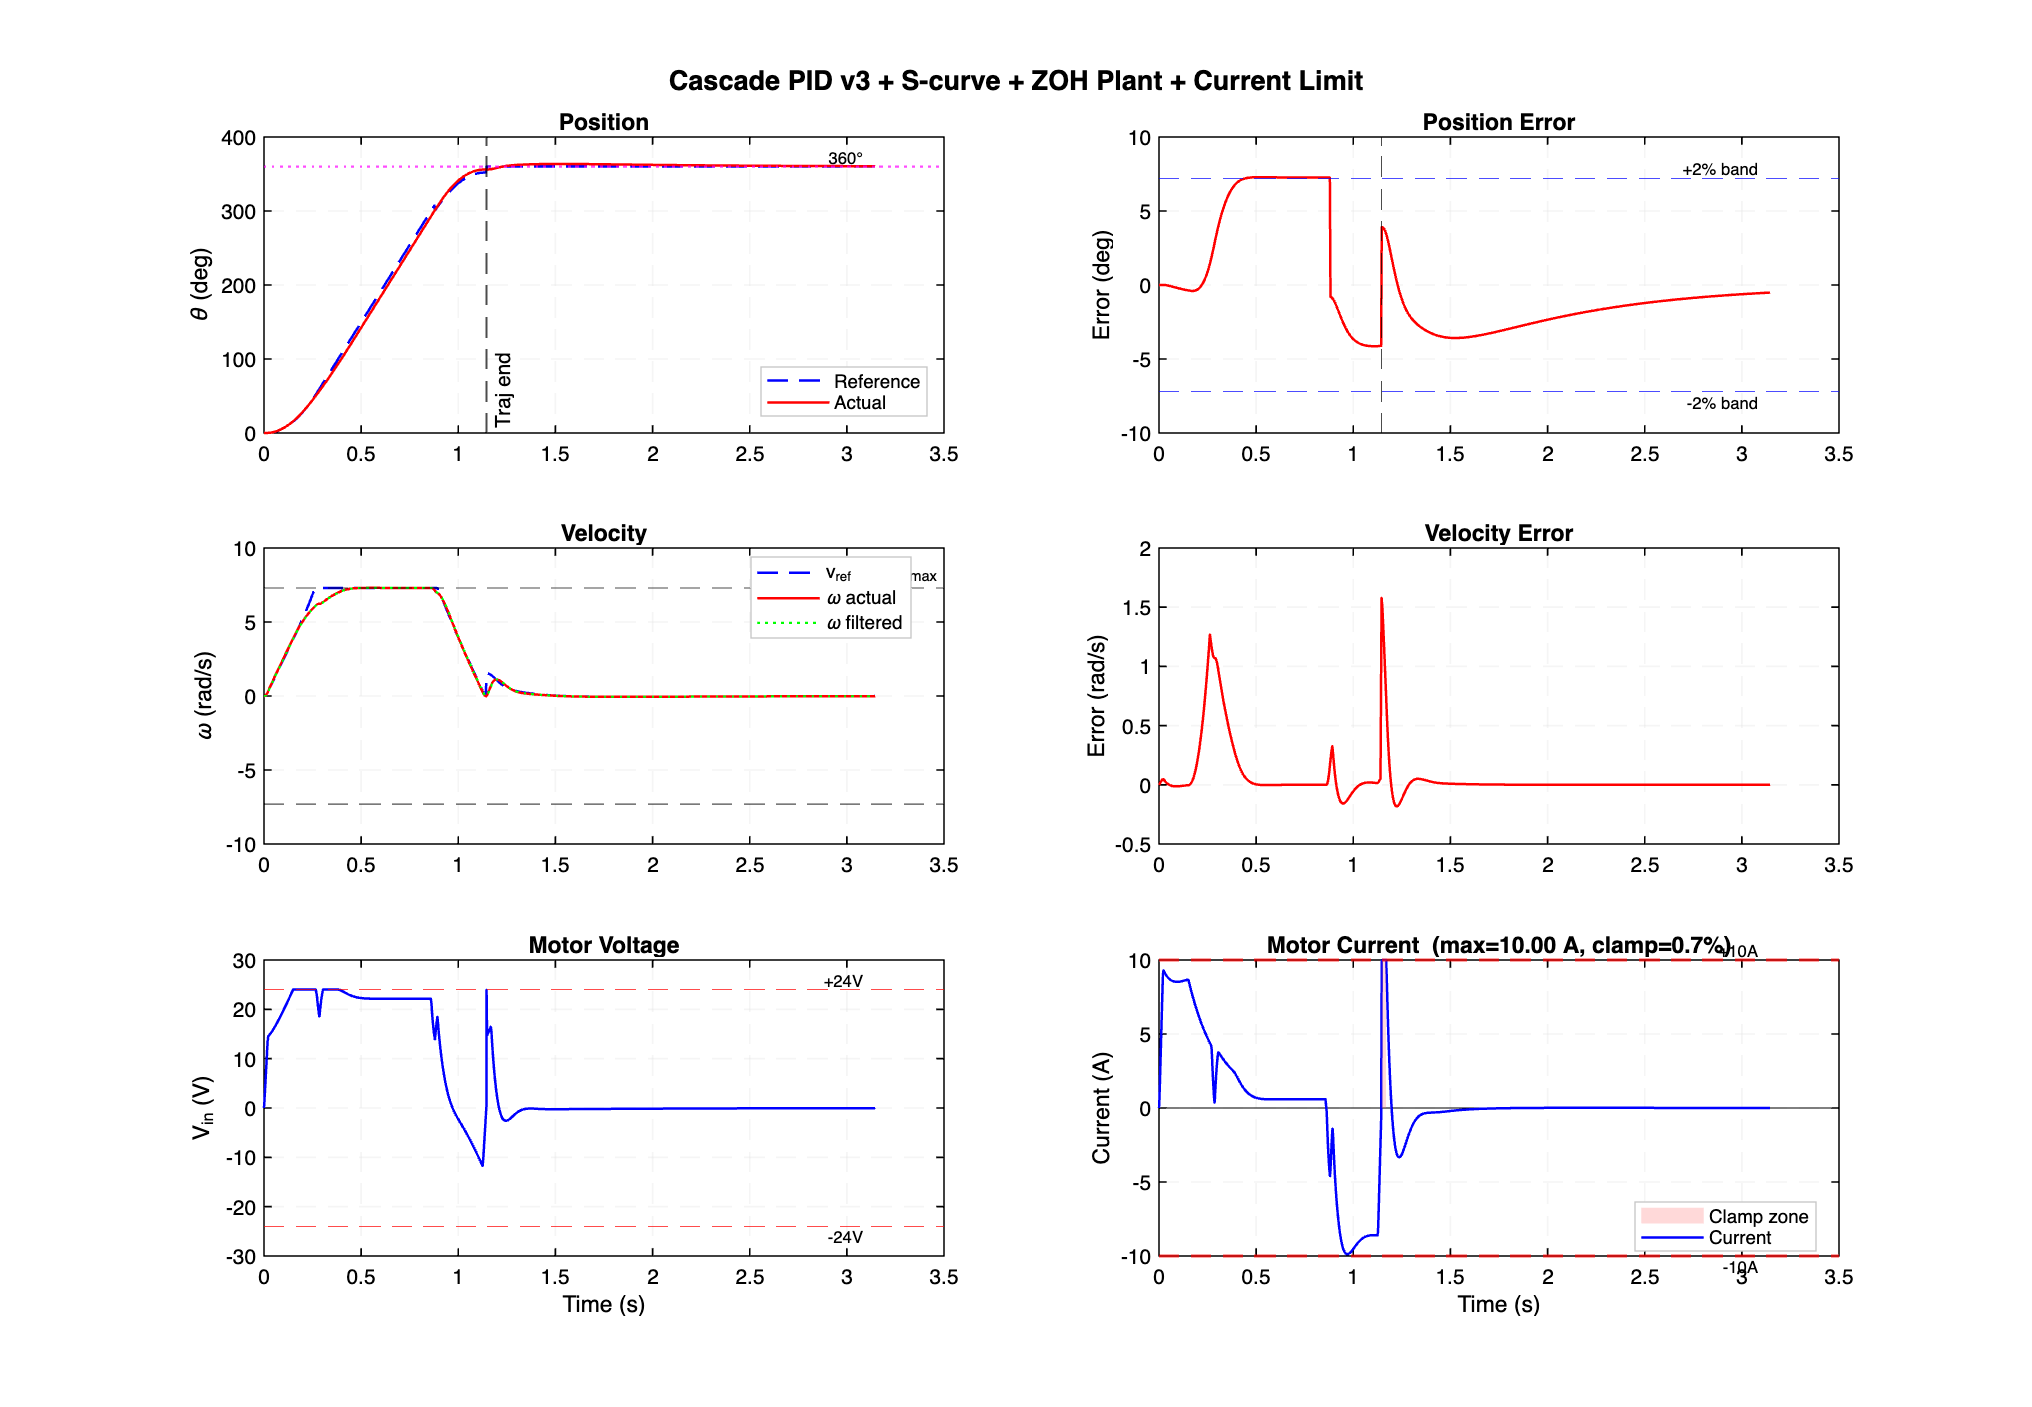
\includegraphics[width=0.95\textwidth]{images/sim_result.png}
  \caption{ผล Simulation: Position, Position Error, Velocity, Velocity Error,
           Motor Voltage และ Motor Current (S-Curve 360°, Cascade PID)}
  \label{fig:sim_result}
\end{figure}

\begin{figure}[H]
  \centering
  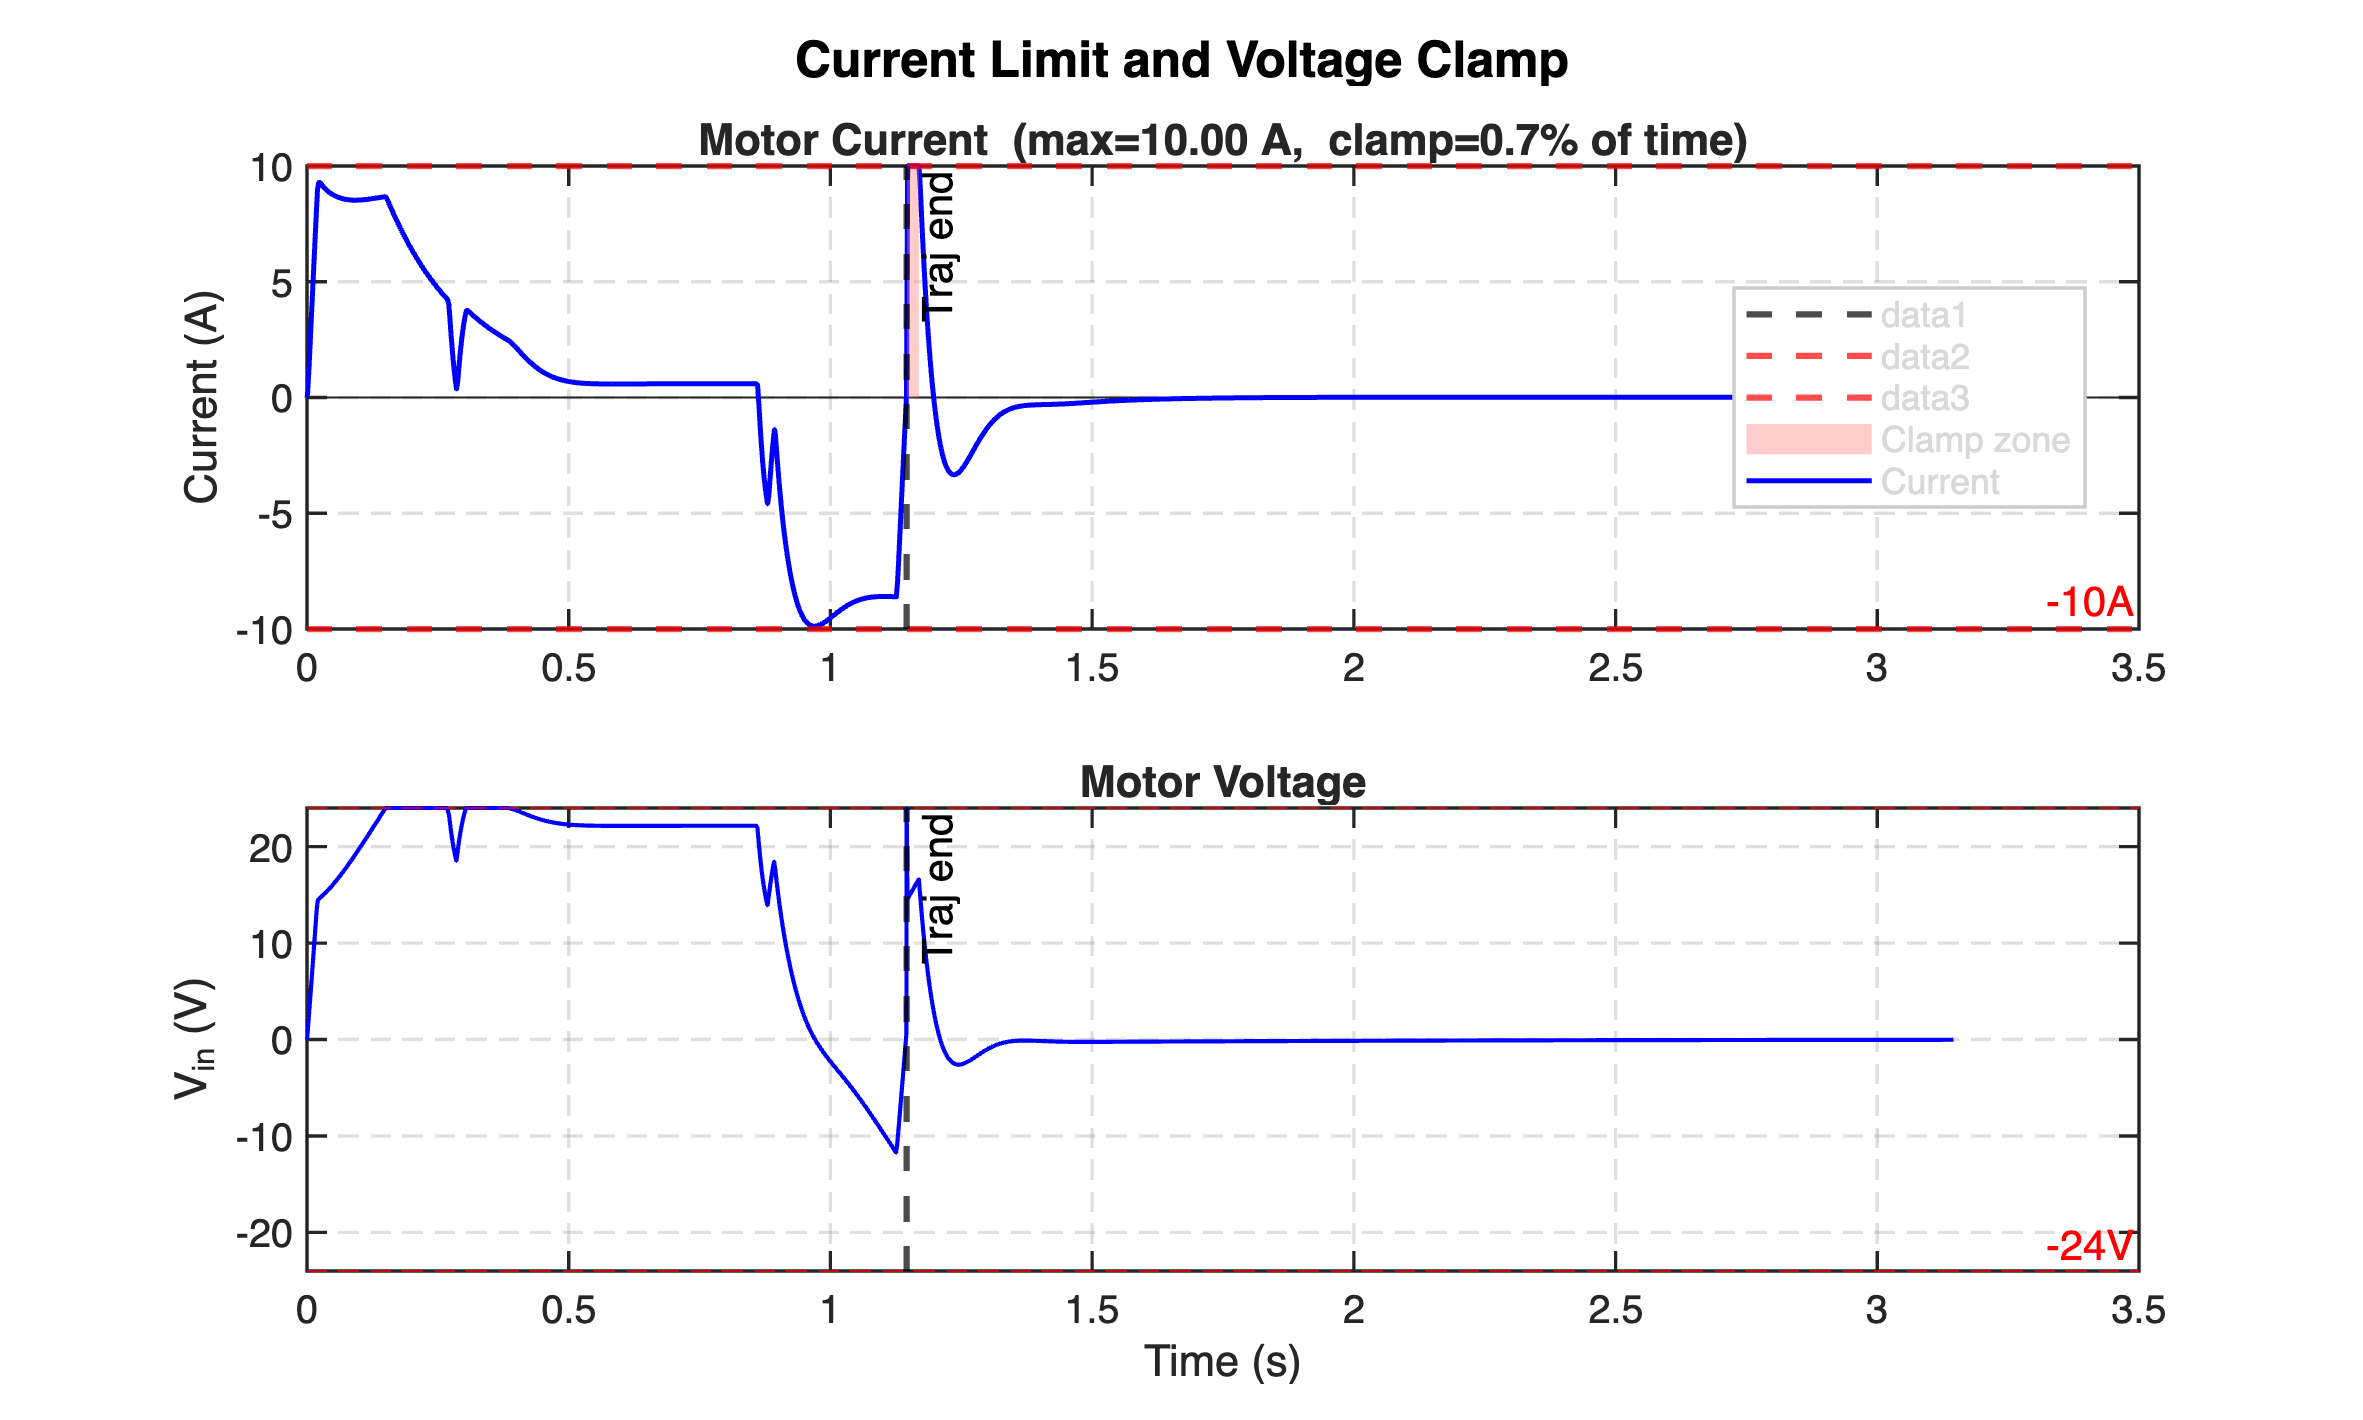
\includegraphics[width=0.78\textwidth]{images/sim_current.png}
  \caption{Motor Current และ Current Clamp Zone ระหว่างการเคลื่อนที่ 360°}
  \label{fig:sim_current}
\end{figure}

\begin{table}[H]
  \centering
  \caption{ผล Simulation เทียบกับ Requirement (S-Curve 360°)}
  \label{tab:sim_vs_req}
  \begin{tabular}{lcccc}
    \toprule
    พารามิเตอร์ & ผล Simulation & Requirement & หน่วย & ผลการตรวจสอบ \\
    \midrule
    Settling Time       & 0.0198  & $\leq 0.5$ & s   & ผ่าน \\
    Overshoot           & 0.9948  & $\leq 1$   & \%  & ผ่าน \\
    Steady-state Error  & 0.512   & --         & deg & -- \\
    Max Current         & 10.00   & $\leq 10$  & A   & ผ่าน \\
    Current Clamp       & 0.71    & --         & \%  & -- \\
    Move Time (360°)    & 1.146   & --         & s   & -- \\
    Cycle Time (4 pcs)  & 22.58   & $\leq 35$  & s   & ผ่าน \\
    \bottomrule
  \end{tabular}
\end{table}

% ============================================================
\subsection{ผลการวิเคราะห์และหาค่าพารามิเตอร์ที่เหมาะสม (Optimization Results)}
\label{subsec:rod_opt_results}
% ============================================================

ผลการวิเคราะห์ Multi-objective Optimization ด้วย NSGA-II เพื่อหาจุดที่เหมาะสมที่สุด (Optimal Solution) ระหว่างเวลาในการทำงาน (Cycle Time) และการแกว่งของชิ้นงาน (Rod Swing)

\begin{figure}[H]
  \centering
  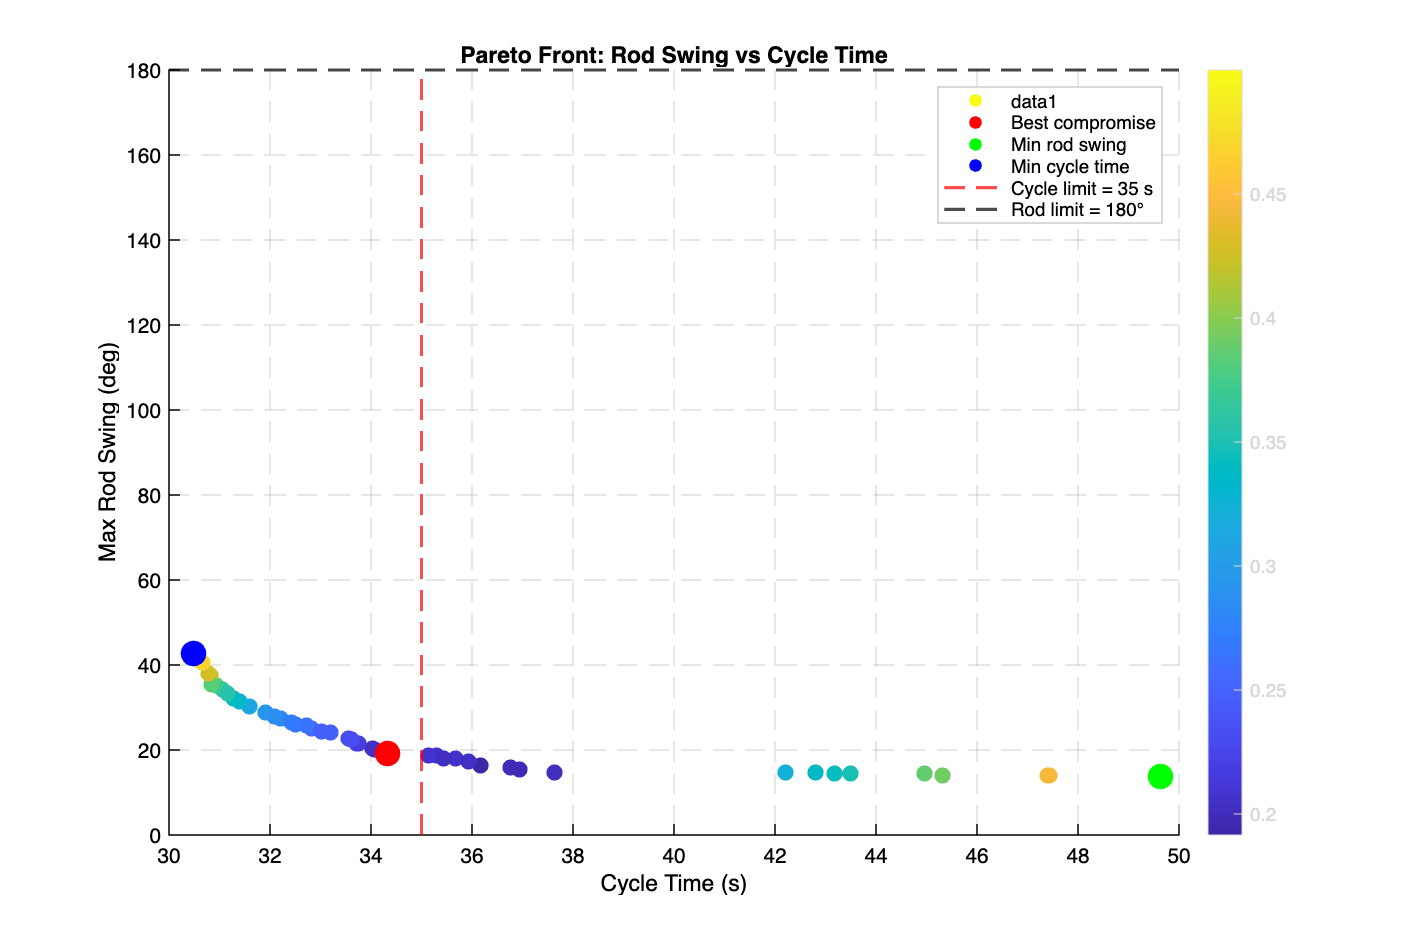
\includegraphics[width=0.88\textwidth]{images/pareto_front.png}
  \caption{Pareto Front จาก NSGA-II แสดง Trade-off ระหว่าง
           Max Rod Swing และ Cycle Time}
  \label{fig:pareto_front}
\end{figure}

\begin{table}[H]
  \centering
  \caption{สรุป Solution บน Pareto Front ที่น่าสนใจ}
  \label{tab:pareto_summary}
  \begin{tabular}{lcccl}
    \toprule
    Solution & Rod Swing (deg) & Cycle Time (s) & ผ่าน 35\,s & หมายเหตุ \\
    \midrule
    ไม่มี Shaping (เดิม)            & 198.0 & $\infty$ & ไม่ผ่าน & Rod ไม่นิ่ง \\
    ZV Shaping (พารามิเตอร์เดิม)   & 84.4  & $\infty$ & ไม่ผ่าน & Rod ไม่นิ่ง \\
    Min Cycle Time                  & 42.7  & 30.5     & ผ่าน    & Rod swing สูง \\
    Best Compromise                 & 19.1  & 34.3     & ผ่าน    & สมดุลดีที่สุด \\
    Min Rod Swing                   & 13.8  & 49.6     & \textbf{ไม่ผ่าน} & เกิน 35\,s มาก \\
    \bottomrule
  \end{tabular}
\end{table}

Solution ที่เลือกใช้คือ ``Best Compromise'' ซึ่งให้ค่าพารามิเตอร์สำหรับการเคลื่อนที่ดังตารางที่~\ref{tab:opt_params} และผลตอบสนองเชิงเวลาดังรูปที่~\ref{fig:rod_best_compromise}

\begin{table}[H]
  \centering
  \caption{ค่าพารามิเตอร์ที่ Optimal จาก NSGA-II (Best Compromise)}
  \label{tab:opt_params}
  \begin{tabular}{lcc}
    \toprule
    พารามิเตอร์ & ค่า & หน่วย \\
    \midrule
    $v_{max}$           & 4.856  & rad/s \\
    $a_{max}$           & 5.960  & rad/s$^2$ \\
    $j_{max}$           & 1085.9 & rad/s$^3$ \\
    $\omega_{n,shaper}$ & 12.386 & rad/s \\
    $\zeta_{shaper}$    & 0.0984 & -- \\
    \midrule
    Rod Swing           & 19.1   & deg \\
    Cycle Time          & 34.3   & s \\
    Arm Settling Time   & 0.067  & s \\
    Overshoot           & 0.018  & \% \\
    Max Current         & 3.62   & A \\
    \bottomrule
  \end{tabular}
\end{table}

\begin{figure}[H]
  \centering
  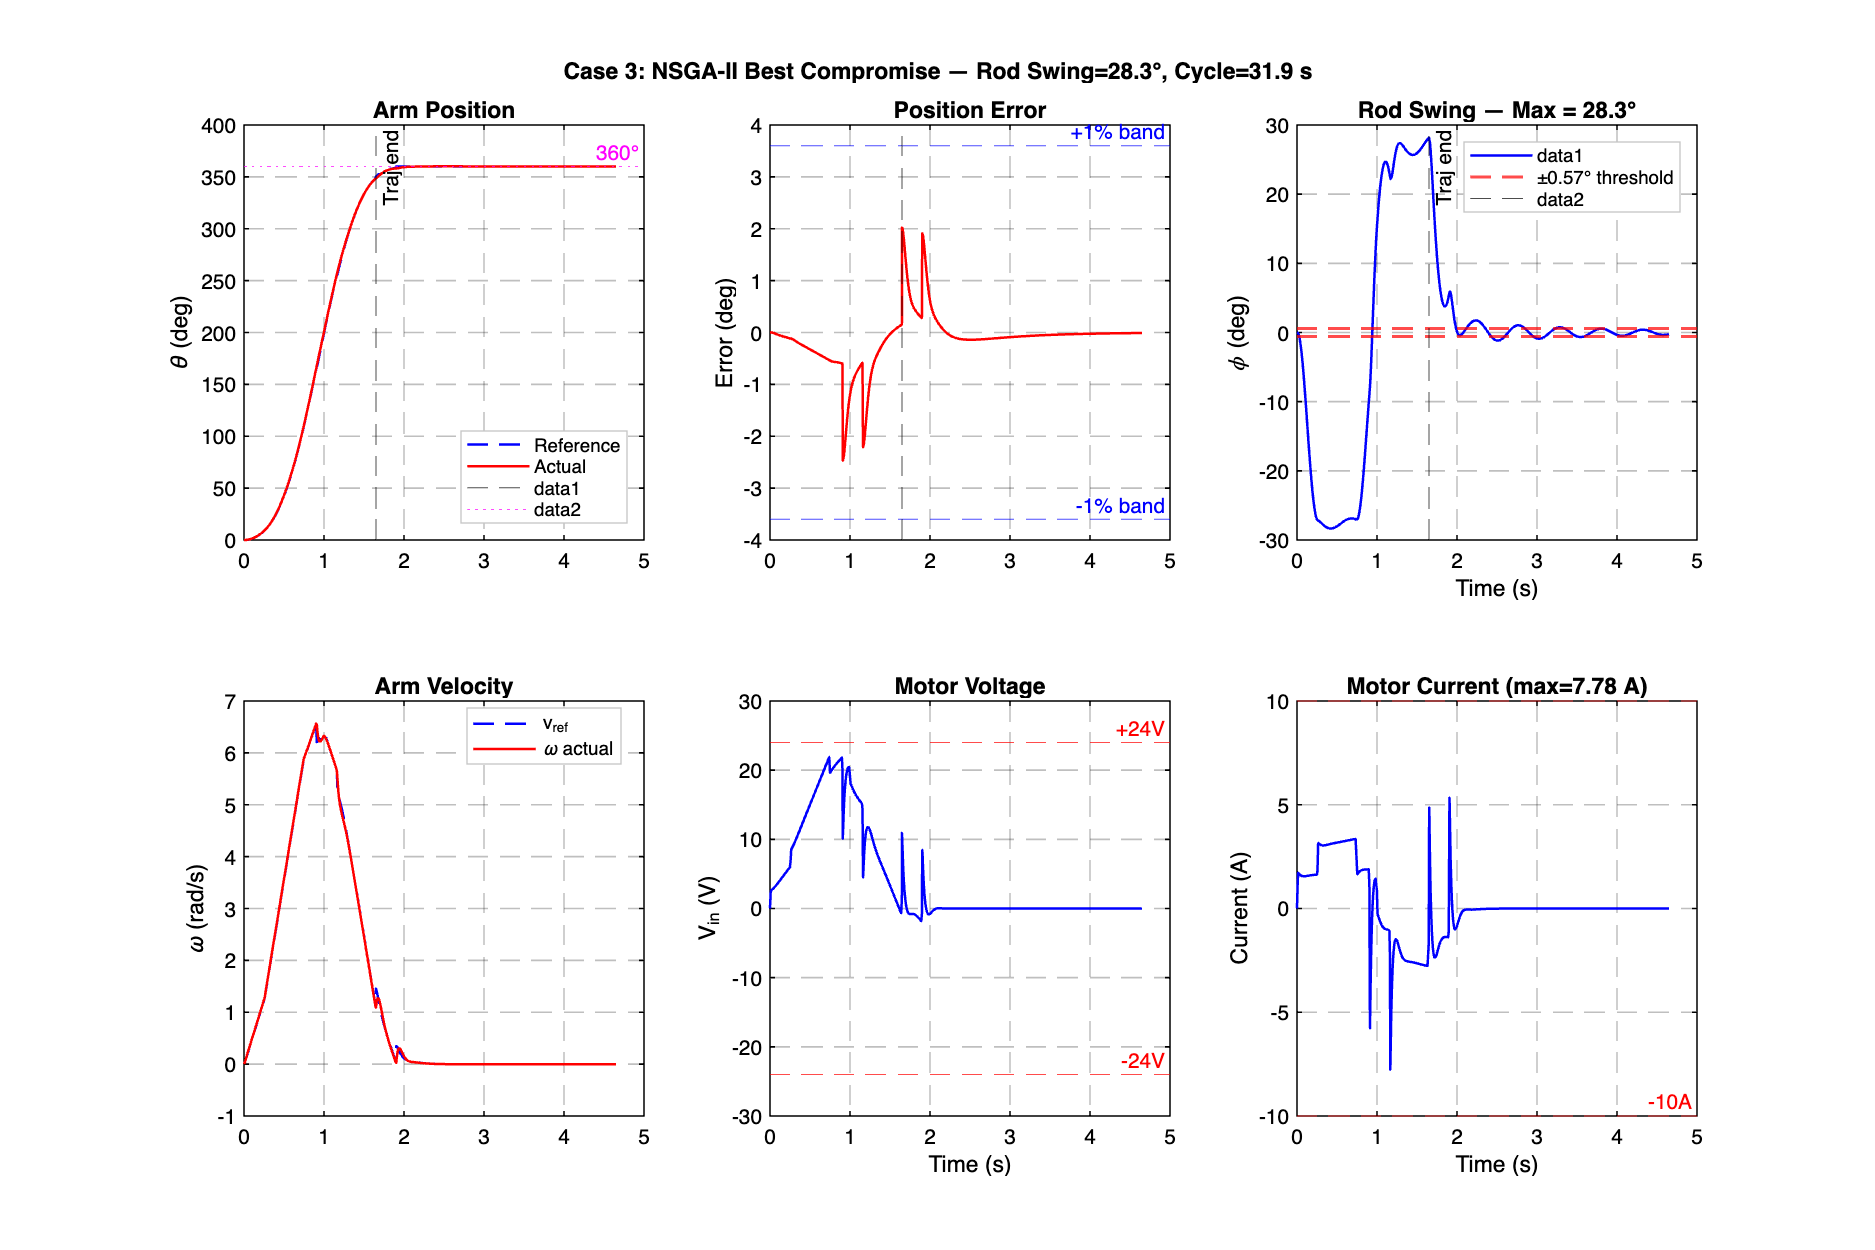
\includegraphics[width=0.88\textwidth]{images/rod_best_compromise.png}
  \caption{ผล Simulation ของ Best Compromise Solution จาก NSGA-II
           (Rod Swing = 19.1°, Cycle Time = 34.3\,s)}
  \label{fig:rod_best_compromise}
\end{figure}

% ============================================================
\subsection{ผลการทดสอบ Progress Update 2 (Unit Tests)}
% ============================================================

\subsubsection{Unit Test: การอ่าน Encoder และ PWM (Deliverable 2)}
...

\begin{table}[H]
  \centering
  \caption{ผล Unit Test Joystick แต่ละโหมด}
  \label{tab:joystick_unit_test}
  % [ตาราง: โหมด | ปุ่มที่กด | การตอบสนอง | Pass/Fail]
\end{table}

\subsubsection{Unit Test: ตู้ควบคุมไฟฟ้า (Deliverable 1)}
% สถานะ: กำลังดำเนินการ --- จะอัปเดต

\subsubsection{การทำ System Identification (Deliverable 6)}
% สถานะ: กำลังดำเนินการ

\begin{table}[H]
  \centering
  \caption{ผล System Identification}
  \label{tab:sysid_result}
  % [ตาราง: พารามิเตอร์ | สัญลักษณ์ | ค่าที่วัดได้ | หน่วย]
  % R_m, L_m, K_e, K_m, J, b --- [ใส่ค่าจริง]
\end{table}

\subsubsection{ผล Simulation Simscape}
% ผล Step Response จาก Simscape ที่ปรับแก้แล้ว (P5, P6)
% ============================================================================
% FILE: sections/06_verification.tex
% PURPOSE: ตาราง V&V ทั้งหมด (Summary รวม + แยกตาม Category)
% ============================================================================

\section{การตรวจสอบและทวนสอบ (Verification and Validation)}

\subsection{ภาพรวม V\&V Framework}
% อธิบายความแตกต่างระหว่าง Verification และ Validation
% อธิบาย Test Method ทั้ง 4: AN, IN, DM, TE

\subsection{ตาราง V\&V รวมทั้งหมด (32 Requirements)}

\begin{table}[H]
  \centering
  \small
  \caption{ตาราง V\&V รวม ทั้ง 32 Requirements}
  \label{tab:vv_summary}
  % [ตาราง 32 แถว: Req ID | Category | คำอธิบาย | Method | Pass Criteria | V&V Type | Status]
  % หากล้นหน้า ให้ใช้ longtable แทน table
\end{table}

\subsection{ตาราง V\&V แยกตาม Category}

\subsubsection{Mechanical Requirements (M1--M10)}

\begin{table}[H]
  \centering
  \small
  \caption{V\&V Table: Mechanical Requirements (M1--M10)}
  \label{tab:vv_mechanical}
  % [ตาราง: Req ID | คำอธิบาย | Method | Pass Criteria | V&V Type | Status | หลักฐาน]
\end{table}

\subsubsection{Performance Requirements (P1--P7)}

\begin{table}[H]
  \centering
  \small
  \caption{V\&V Table: Performance Requirements (P1--P7)}
  \label{tab:vv_performance}
\end{table}

\subsubsection{Accuracy Requirements (A1--A5)}

\begin{table}[H]
  \centering
  \small
  \caption{V\&V Table: Accuracy Requirements (A1--A5)}
  \label{tab:vv_accuracy}
\end{table}

\subsubsection{Electrical Requirements (E1--E9)}

\begin{table}[H]
  \centering
  \small
  \caption{V\&V Table: Electrical Requirements (E1--E9)}
  \label{tab:vv_electrical}
\end{table}

\subsubsection{Joystick Requirements (J1)}

\begin{table}[H]
  \centering
  \small
  \caption{V\&V Table: Joystick Requirements (J1)}
  \label{tab:vv_joystick}
\end{table}

\subsection{สรุปสถานะ V\&V ตาม Category}

\begin{table}[H]
  \centering
  \caption{สรุปสถานะ V\&V แยกตาม Category}
  \label{tab:vv_status_summary}
  % [ตาราง: Category | Total | VER | VAL | VER+VAL | PASS | FAIL | PENDING | Pass Rate]
  % Mechanical  | 10 | 8 | 1 | 1 | 0 | 0 | 10 | 0%
  % Performance |  7 | 6 | 0 | 1 | 0 | 0 |  7 | 0%
  % Accuracy    |  5 | 5 | 0 | 0 | 0 | 0 |  5 | 0%
  % Electrical  |  9 | 9 | 0 | 0 | 0 | 0 |  9 | 0%
  % Joystick    |  1 | 0 | 0 | 1 | 0 | 0 |  1 | 0%
  % TOTAL       | 32 |28 | 1 | 3 | 0 | 0 | 32 | 0%
\end{table}
% ============================================================================
% FILE: sections/07_conclusion.tex
% PURPOSE: สรุปผล แยกตาม Progress 1 / Progress 2 / Future Work
% ============================================================================

\section{สรุปผลและแนวทางต่อไป (Conclusion)}

\subsection{สรุปผลงาน Progress Update 1}
% สิ่งที่ทำสำเร็จใน P1 และปัญหาที่พบ
% - ผล FEA และการคำนวณ Mechanical (Shaft, Belt, Bearing, Deflection)
% - Motion Profile ทฤษฎี 34.39 s ผ่านเกณฑ์ P1
% - ปัญหาที่พบและวิธีแก้ไข

\subsection{สรุปผลงาน Progress Update 2}
% สิ่งที่ทำสำเร็จใน P2 และปัญหาที่พบ
% - STM32 อ่าน Encoder, ส่ง PWM สำเร็จ (Deliverable 2)
% - PID Closed-Loop + S-Curve ทำงานได้ (Deliverable 3) รอ Tune
% - Joystick ทุกโหมดสำเร็จ (Deliverable 4)
% - ตู้ไฟ กำลังดำเนินการ (Deliverable 1)
% - Modbus กำลังดำเนินการ (Deliverable 5)
% - System ID กำลังดำเนินการ (Deliverable 6)
% - ปัญหาที่พบและวิธีแก้ไข

\subsection{แนวทางและแผนงานต่อไป (Future Work)}
% สิ่งที่ต้องทำก่อน Final Demo (Demo 1: 1 มิ.ย. / Demo 2: 8 มิ.ย.)
% - ทำ System ID ให้เสร็จ รับค่าพารามิเตอร์จริง
% - ออกแบบ PID จาก Root Locus รับค่า Kp, Ki, Kd
% - Tune PID บน Hardware จริง
% - เชื่อมต่อ Modbus กับ Base System
% - ประกอบตู้ไฟให้เสร็จและทำ Unit Test
% - End-to-End Test ทั้งระบบ
% - ทดสอบ V&V ทั้ง 32 Requirement
% ============================================================================
% FILE: sections/08_appendix.tex
% PURPOSE: รายละเอียดเพิ่มเติมที่ไม่ได้ใส่ในเนื้อหาหลัก
% ============================================================================

\appendix

\section{รายละเอียดการคำนวณเชิงกล}
% การคำนวณฉบับเต็ม Shaft, Belt, Bearing, Deflection
% อ้างอิงไฟล์ PDF ที่มีอยู่แล้วใน Project

\section{รายละเอียดการคำนวณ Motion Profile}
% การคำนวณ S-Curve ฉบับเต็ม ทุกช่วง (Acceleration, Constant, Deceleration)

\section{Schematic ไฟฟ้าฉบับเต็ม}
% Schematic ขนาดเต็มอ่านได้ง่าย

\begin{figure}[H]
  \centering
%   \includegraphics[width=0.95\textwidth]{images/schematic_full.png}
  % [ใส่ภาพ Schematic ขนาดเต็ม]
  \caption{Electrical Schematic ฉบับเต็ม}
  \label{fig:schematic_full}
\end{figure}

\section{Code Snippet หลักของ STM32 Firmware}
% Code สำคัญ เช่น PID Loop, Encoder Read, S-Curve Generator
% ใช้ lstlisting environment

\begin{lstlisting}[language=C, caption={ตัวอย่าง PID Control Loop บน STM32}]
/* [ใส่ Code จริงของ PID Loop] */
\end{lstlisting}

\section{ผลการ Simulation Simscape ฉบับเต็ม}
% Plot และผลลัพธ์จาก Simscape ทุก Scenario

\begin{figure}[H]
  \centering
%   \includegraphics[width=0.85\textwidth]{images/simscape_full_result.png}
  % [ใส่ Plot ทั้งหมดจาก Simscape: Position, Velocity, Control Effort]
  \caption{ผล Simulation Simscape ฉบับเต็ม}
  \label{fig:simscape_full}
\end{figure}

\section{Log การทดสอบ Unit Test}
% Serial Log, Oscilloscope Screenshot จากการทดสอบต่างๆ

\begin{figure}[H]
  \centering
%   \includegraphics[width=0.80\textwidth]{images/serial_log_encoder.png}
  % [ใส่ภาพ Serial Monitor Log แสดงค่า Encoder ขณะทดสอบ]
  \caption{Serial Log ขณะทดสอบการอ่านค่า Encoder}
  \label{fig:serial_log}
\end{figure}

% ----------------------------------------------------------------------------
% 9. Bibliography
% ----------------------------------------------------------------------------
\nocite{*}
\bibliographystyle{apalike}
\bibliography{references}

\end{document}

\newpage
\appendix